% !TeX spellcheck = en_US
% arara: pdflatex
% arara: bibtex
% arara: pdflatex
% arara: pdflatex
\documentclass[journal,10pt,twoside]{IEEEtran}
\usepackage[utf8]{inputenc}
\usepackage{times,textcomp,amssymb}
\usepackage[cmex10]{amsmath}
\usepackage[T1]{fontenc}
\usepackage[english]{babel}

\usepackage{breqn,cite}
%\usepackage{epstopdf}
\usepackage[dvipsnames]{xcolor}
\usepackage[pdftex]{graphicx}
\usepackage{subfig}
\usepackage[justification=centering]{caption}
\usepackage[section]{placeins} % floats never go into next section
%\let\labelindent\relax % Compact lists
\usepackage{array,booktabs,enumitem,balance} % nice rules in tables

% amsmath sets \interdisplaylinepenalty = 10000
% preventing page breaks from occurring within multiline equations
\interdisplaylinepenalty=2500

%tikz figures
\usepackage{tikz}
\usetikzlibrary{automata,positioning,chains,shapes,arrows}
\usepackage{pgfplots}
\usetikzlibrary{plotmarks}
\newlength\fheight
\newlength\fwidth
\pgfplotsset{compat=newest}
\pgfplotsset{plot coordinates/math parser=false}

\newcommand{\EB}[1]{\textit{\color{blue}EB says: #1}}
\newcommand{\FR}[1]{\textit{\color{ForestGreen}FR says: #1}}
\newcommand{\LA}[1]{\textit{\color{orange}LA says: #1}}
\newcommand{\FS}[1]{\textit{\color{red}FS says: #1}}

\usepackage{hyperref}
\definecolor{dkpowder}{rgb}{0,0.2,0.7}
\hypersetup{%
    pdfpagemode  = {UseOutlines},
    bookmarksopen,
    pdfstartview = {FitH},
    colorlinks,
    linkcolor = {dkpowder},
    citecolor = {dkpowder},
    urlcolor  = {dkpowder},
}
\addto\extrasenglish{%
  \renewcommand{\sectionautorefname}{Section}%
  \renewcommand{\subsectionautorefname}{Subsection}%
}

\pdfminorversion=7 % fixes warnings of eps to pdf included images

%%%%%%%%%%%%%%%%
\begin{document}
\title{A study on the Iterated Prisoner's Dilemma}

\author{%
    \IEEEauthorblockN{Elia Bonetto, Filippo Rigotto, Luca Attanasio and Francesco Savio}

    \IEEEauthorblockA{Department of Information Engineering, University of Padova -- Via Gradenigo, 6/b, 35131 Padova, Italy}
    % \\Email: {\tt\{bonettoe,rigottof,attanasiol,saviofranc\}@dei.unipd.it}}
}
\markboth{Laboratory of Computational Physics, Fall 2018}%
    {Bonetto \MakeLowercase{\textit{et al.}}: A study on the Iterated Prisoner's Dilemma}

\maketitle
%%%%%%%%%%

\begin{abstract}
% matching = accoppiamento
In this work, the popular Iterated Prisoner's Dilemma game is analyzed in different matching scenarios: (i) the classical version between two players, (ii) a generalization of the classical version between multiple players, (iii) an extension of (ii) allowing the population of players to evolve or (iv) allowing players' strategies to randomly change between rounds, according to a gene representing the grade of cooperation. % (a Nature choice, in Game Theory terms).
Rounds' statistics are collected to have an insight on which is the best strategy, if there is an absolute winner, which is the evolution and which is the players' score of each scenario.
\end{abstract}

\section{Introduction} \label{s:intro}
\IEEEPARstart{T}{he} Prisoner's Dilemma (PD) is a classical game analyzed in Game Theory which attempts to model social and economical interactions. It is a \textit{dilemma} because, if exploited to explain the emergence of altruism in human society or, generally, in animal society, it fails badly at a first glance. The game is based on a couple of players who have to make a decision on whether to cooperate or not with their opponent. As we will see shortly, even if the intuition tells us that the best choice is to \textit{cooperate}, the only win-ever strategy in a one-shot game is  \textit{not} to cooperate (\textit{defect}).

More insights on this aspect can be found in \autoref{s:game} which gives a theoretical and mathematical introduction on the Prisoner's Dilemma problem and on its iterated version.
In \autoref{s:str}, we illustrate the strategies (the definitions of the players' ways of acting) we have implemented among all the possible ones.
Furthermore, in Sections [\ref{s:IPD2P}, \ref{s:IPDMP}, \ref{s:rIPDMP}, \ref{s:crIPDMP}] we explore the results of the simulations for each study-case.
\autoref{s:ml} is about a brief introduction and review of related works approaching the problem by using machine learning and artificial intelligence procedures, such as reinforcement learning and evolutionary algorithms.
Eventually, in \autoref{s:conc}, some final considerations summarizing the analysis are presented.
All the tables of tournament results, statistics and additional figures can be found in the \hyperref[s:appendix]{Appendix}.

All the code, developed in \textit{Python 3}, is available on \href{https://github.com/eliabntt/LaboratoryOfComputationalPhysics/tree/Group9}{GitHub}.

\section{The dilemma explained} \label{s:game}
The classical formulation of the PD implies that given two prisoners in a scenario where their conviction depends on their mutual cooperation, they can either stay silent or fink, respectively cooperate or defect.
Another possible formulation is by means of a trade-off game, the \textit{closed bag exchange}:

\begin{quote}
\textit{Two people meet and exchange closed bags, with the understanding that one of them contains money and the other contains a purchase. Either player can choose to honor the deal by putting into his or her bag what he or she has agreed, or he or she can defect by handing over an empty bag.}
\end{quote}

Mathematically, the PD can be expressed with linear algebra. The key component is the \textit{Payoff matrix} $M$, which quantifies the reward of each player depending on whether he\footnote{For the rest of the paper, the player is considered a male, for the sake of simplicity in writing. Of course, nothing changes assuming a female player.} cooperated or defected:
$$
M = 
\begin{pmatrix} 
R & S \\
T & P 
\end{pmatrix}
$$
where $T$ (Temptation), $R$ (Reward), $S$ (``Sucker's''), $P$ (Punishment) are integer numbers that satisfy the following conditions, as proven by Rapoport~\cite{rapoport}:
$$
T>R>P>S; \quad 2R > T+S 
$$
For example, $T=3$, $R=2$, $P=1$ and $S=0$, or  $T=5$, $R=3$, $P=1$, $S=0$, the default for all our experiments.

$R$ is returned for both players if they both cooperate, $P$ if they both defect; if the two players' actions differ, $S$ is for the player who cooperated and $T$ is for the one who defected.

Similarly, each player's choice (move or action) for a single round can be represented by one of the two axis in $\mathbb{R}^2$, i.e. $u_C=\begin{pmatrix} 1 \\ 0 \end{pmatrix}$ or $u_D=\begin{pmatrix} 0 \\ 1 \end{pmatrix}$, where the first axis stands for \textit{Cooperate} and the second for \textit{Defect}. Being $u_1$ and $u_2$ the moves of the first and second player respectively, their rewards $r_1$ and $r_2$ can then be computed as:
$$
r_1 = u_1^T M u_2
\quad
\quad
r_2 = u_2^T M u_1
$$

For a single-shot game, namely a game which is played only once, the best strategy (choice of action) may seem for both players to cooperate. If both players cooperate, this leads to a good payoff which maximizes the global outcome, evaluated as the sum of the payoffs for each of them. This is indeed the \textit{Pareto dominating strategy}.

Here lies the dilemma: when a player is facing the decision to cooperate or not, if he chooses to cooperate, he also realizes that the best choice of action would have been instead to betray the other player as this leads, \textit{irrespective of the opponent's move}, to a better payoff for itself.

Both players are rational, which also implies some degree of selfishness, and that they are fully aware of the rules of the game (they have \textit{common knowledge}, using Game Theory terms). In addition, they move simultaneously (so no one knows the opponent's move beforehand). Provided these statements and by doing the simple reasoning explained above, the two players will conclude that the best way of acting is to defect: this would lead to a slightly lower payoff if the opponent defects (minor punishment), but to a higher one if the other player chooses to cooperate, allowing them both to gain something in any case, instead of risking to loose everything.

As a result, the only reasonable conclusion is that the only \textit{Nash Equilibrium}, or the only way to always win this game in a single-shot scenario, is to defect.

Thus, we have just observed that the \textit{Nash Equilibrium} is not \textit{Pareto optimal}: playing cooperate is not feasible since the player is in danger against a defecting opponent. Hence, the only strategy in which nobody wants to deviate is to defect, as also noted by Fogel~\cite{fogelEvolvingBehaviors}.

If repeated games are taken into consideration, this reasoning could loose some meaning. In particular, this is the case of the multiplayer Iterated Prisoner Dilemma (IPD), since time and memory (history) must be considered and the combination of the players may have some unexpected outcomes.
Colman supported this concept by indicating that the 2-player IPD is different from the generalized N-player version, and that strategies that work well in the first scenario may fail in large groups.~\cite{yao1994experimental}
In addition, Grim Triggers, Tit For (Two) Tat, random or even more articulated strategies can be introduced, changing the balance of the game and of the previously defined winning cases.
Moreover, in this game, or more generally in iterated games, the notions of Nash Equilibrium, Pareto optimal or evolutionary stable strategies\footnote{A strategy is said to be \textit{evolutionary stable} if it cannot be overwhelmed by the joint effect of two or more competing strategies. As a matter of fact, Lorberbaum, Boyd, Farrell and Ware proved that no pure or mixed strategy is ev. stable in the long run, if future moves are discounted (see~\cite{lorb94}).} do not suggest new, efficient and interesting strategies since they inherently loose some meaning due to the intrinsic nature of iterated games.~\cite{mathieu2017}
Winning a game in this setup simply means eventually achieving a better payoff with respect to the opponents and this could be carried out even without playing such strategies.

\section{Strategies} \label{s:str}
The strategy is represented as a function which outputs either $u_C$ or $u_D$. Based on the strategy, such function might depend on one or both players' history of moves, or on the number of moves played up to that moment and so on.
The strategy is based on a probability density function. In this project both probabilistic and deterministic strategies are used.

The strategies based on probability are:
\begin{description}
    \item[Nice guy] always cooperate (function's output is always $u_C$).
    \item[Bad guy] always defect (function's output is always $u_D$).
    \item[Mainly nice] randomly defect $k\%$ of the times, $k<50$.
    \item[Mainly bad] randomly defect $k\%$ of the times, $k>50$.
    \item[Indifferent] randomly defect half $(k=50\%)$ of the times.
\end{description}

The deterministic strategies are:
\begin{description}
    \item[Tit-for-Tat (TfT)] start by cooperating the first time, then repeat opponent's previous move.
    \item[Tit-for-Two-Tat (Tf2T)] cooperate the first two times, then defect only if the opponent defected last two times.
    \item[Grim-Trigger (GrT)] always cooperate until the opponent's first defect move, then always defect. 
\end{description}

The strategies are considered static in case they apply the same move at each iteration as in \textit{Nice guy}, \textit{Bad guy} and dynamic elsewhere.
These players' strategies are generally fixed in time, i.e. a player cannot change its strategy between rounds, unless specifically requested by the study case rules.
Many more and much complicated strategies could be analyzed and our implementation is open and structured so that it can be easy to add one strategy just by changing a couple of lines in the code.

\section{Two players IPD} \label{s:IPD2P}
In this section, the IPD intercourse between two players is evaluated: each player has an assigned strategy, he is unaware of the opponent's way of acting and he plays accordingly to its strategy definition without the possibility to change it. Both players know only their respective history of choices. Each game is repeated for a fixed number of rounds, unknown to the two players. The main metric evaluated as output of this game is the winner, or in other words the one who achieves a higher payoff at the end of the round.

The number of iterations was fixed to \texttt{NUM\_ITER = 50} and can be modified by means of a simple option when launching the program.
This could also be seen as the number of moves during the match, and is a factor unknown to the players; if otherwise, a smart player could adopt a supposedly optimal strategy: for example, against a \textit{Nice} (or \textit{TfT}) strategy the best choice of action\footnote{As inferred from \textit{backward induction} reasoning.} would be to cooperate in all but the last round, gaining advantage from knowing the number of runs.
Results do not depend on this value if only deterministic strategies are employed; conversely, it will slightly influence the random ones.
Note that in every simulation, a \texttt{seed} value is fixed, so as to have reproducible results from the pseudo-random number generator.

All the possible combinations between players, which represents each strategy presented in \autoref{s:str}, are evaluated, including the case in which the player plays against itself (or, similarly, against a player with the same strategy).
This is a simple repetition of the single-shot game with the addition of memory and the possibility to add probabilistic and more elaborated strategies, as it has already been highlighted.

Since the population is not a concern in this study-case (which is a single A vs B game), the winning strategy in all cases is to \textit{not} cooperate, or, in other terms, the \textit{Always Bad guy} strategy, as expected.

As a matter of fact, in all scenarios, \textit{Bad guy} reaches at least the same reward of the opponent, but more often it gets a higher one as in Figures~[\ref{fig:badvstft},\ref{fig:badvsnice},\ref{fig:badvsmainlybad}]. 
Furthermore, a game facing a \textit{Bad guy} against another \textit{Bad guy} as in \autoref{fig:badvsbad}, or similarly against a \textit{Mainly bad} (\autoref{fig:badvsmainlybad}), leads to the same cumulative reward for both players in the former case or almost the same in the latter. The obtained reward is not as good as if players were playing against (mainly) nice strategies.
This is a first important insight that verifies and points out what has been seen from a theoretical point of view earlier: defecting is always a winning strategy, but it may be non-optimal; on the other hand, if both are cooperating, so playing the Pareto Optimal combination, each of them gains more in terms of payoff and would get an advantage if they choose to defect against the other. In the latter case, memory is important as it allows revenge and reactive strategies to exist, keeping in mind that the total number of rounds is unknown. 

\begin{figure}[!ht]
    \centering
    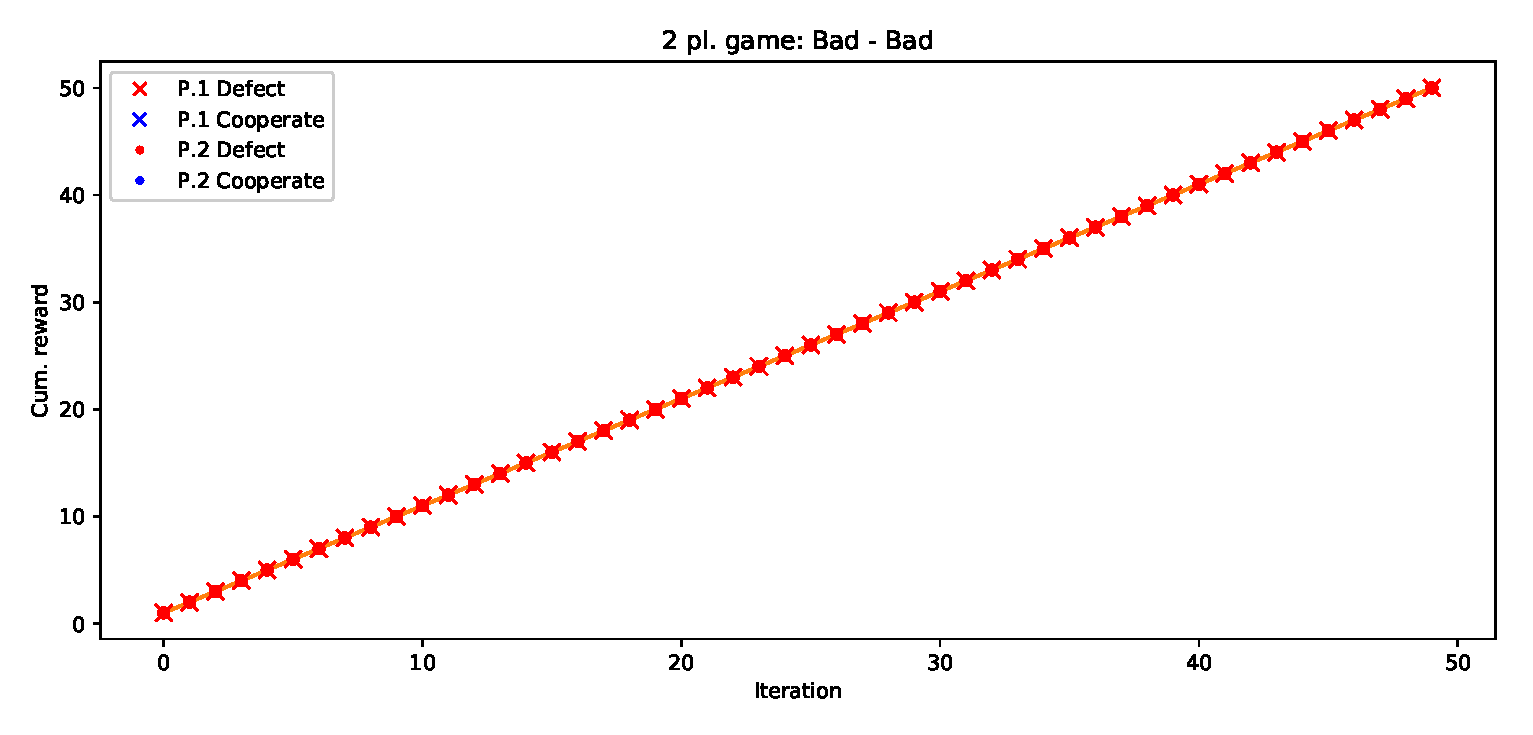
\includegraphics[width=.9\columnwidth]{../img/ipd2p/ipd2p-rewards-Bad-Bad}
    \caption{Bad vs Bad}
    \label{fig:badvsbad}
\end{figure}

\begin{figure}[!ht]
    \centering
    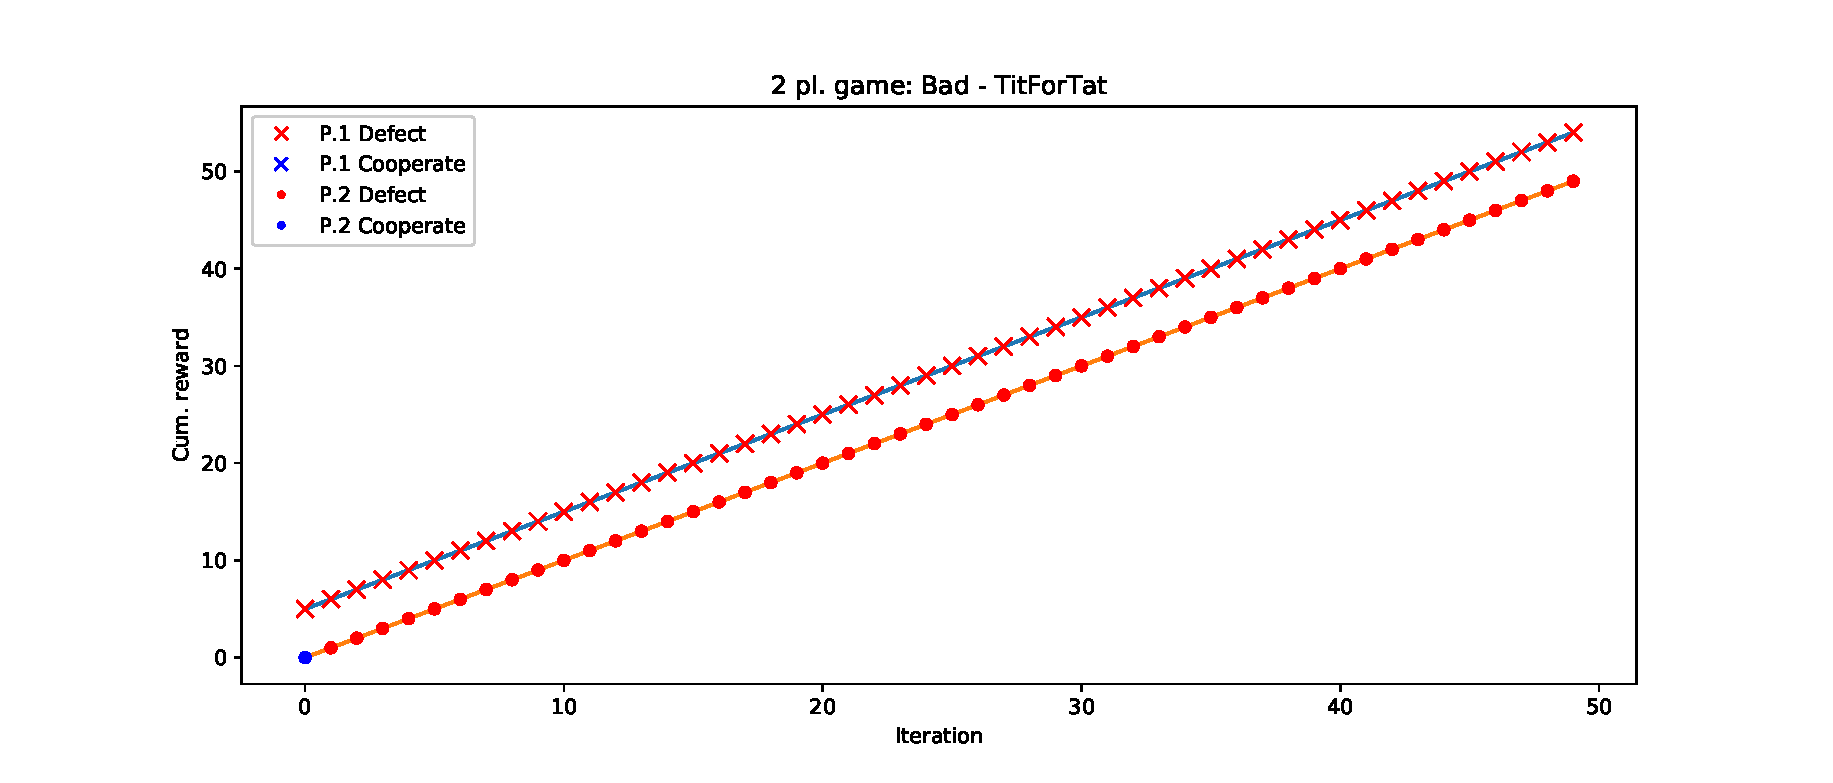
\includegraphics[width=.9\columnwidth]{../img/ipd2p/ipd2p-rewards-Bad-TitForTat}
    \caption{Bad vs TfT}
    \label{fig:badvstft}
\end{figure}

\begin{figure}[!ht]
    \centering
    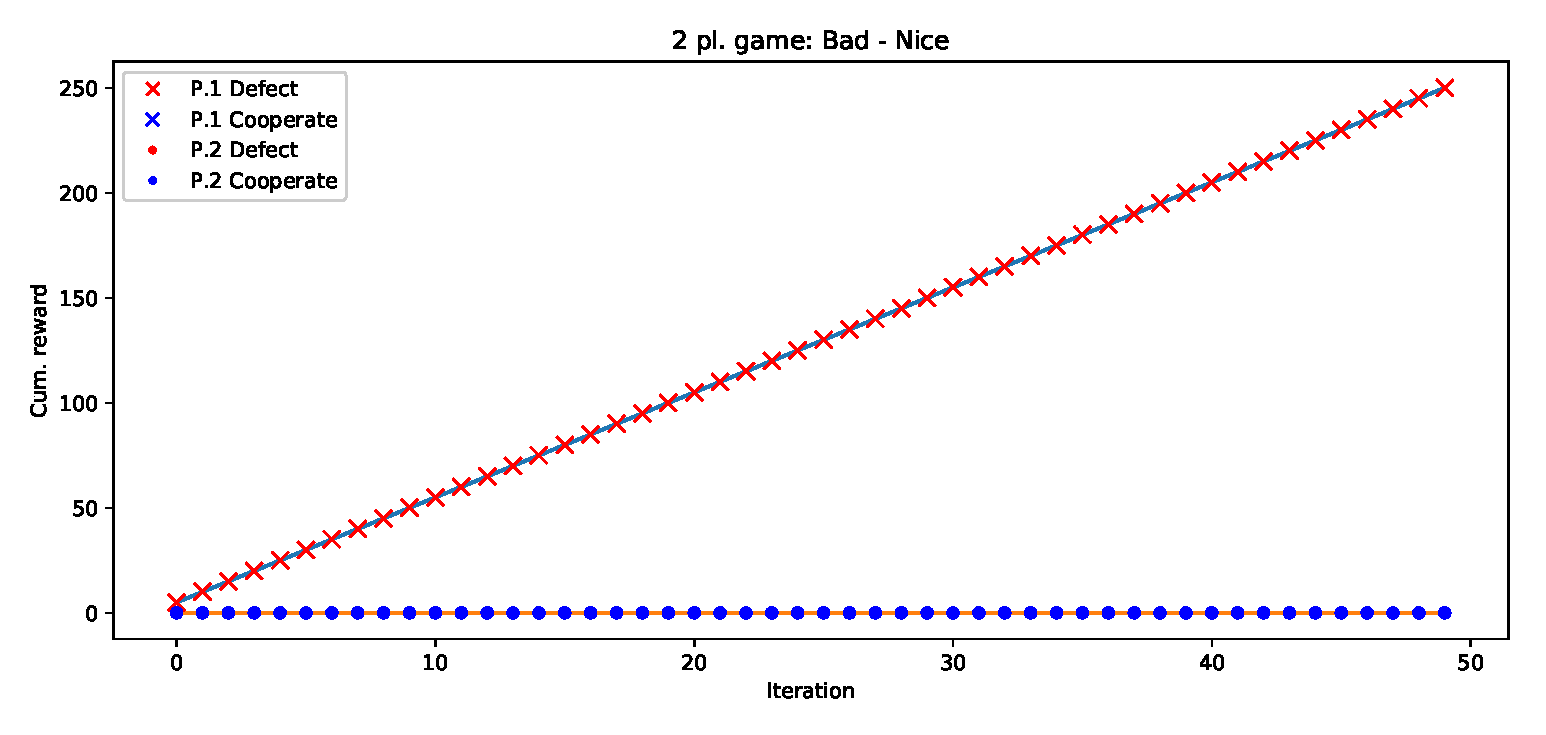
\includegraphics[width=.9\columnwidth]{../img/ipd2p/ipd2p-rewards-Bad-Nice}
    \caption{Bad vs Nice}
    \label{fig:badvsnice}
\end{figure}

\begin{figure}[!ht]
    \centering
    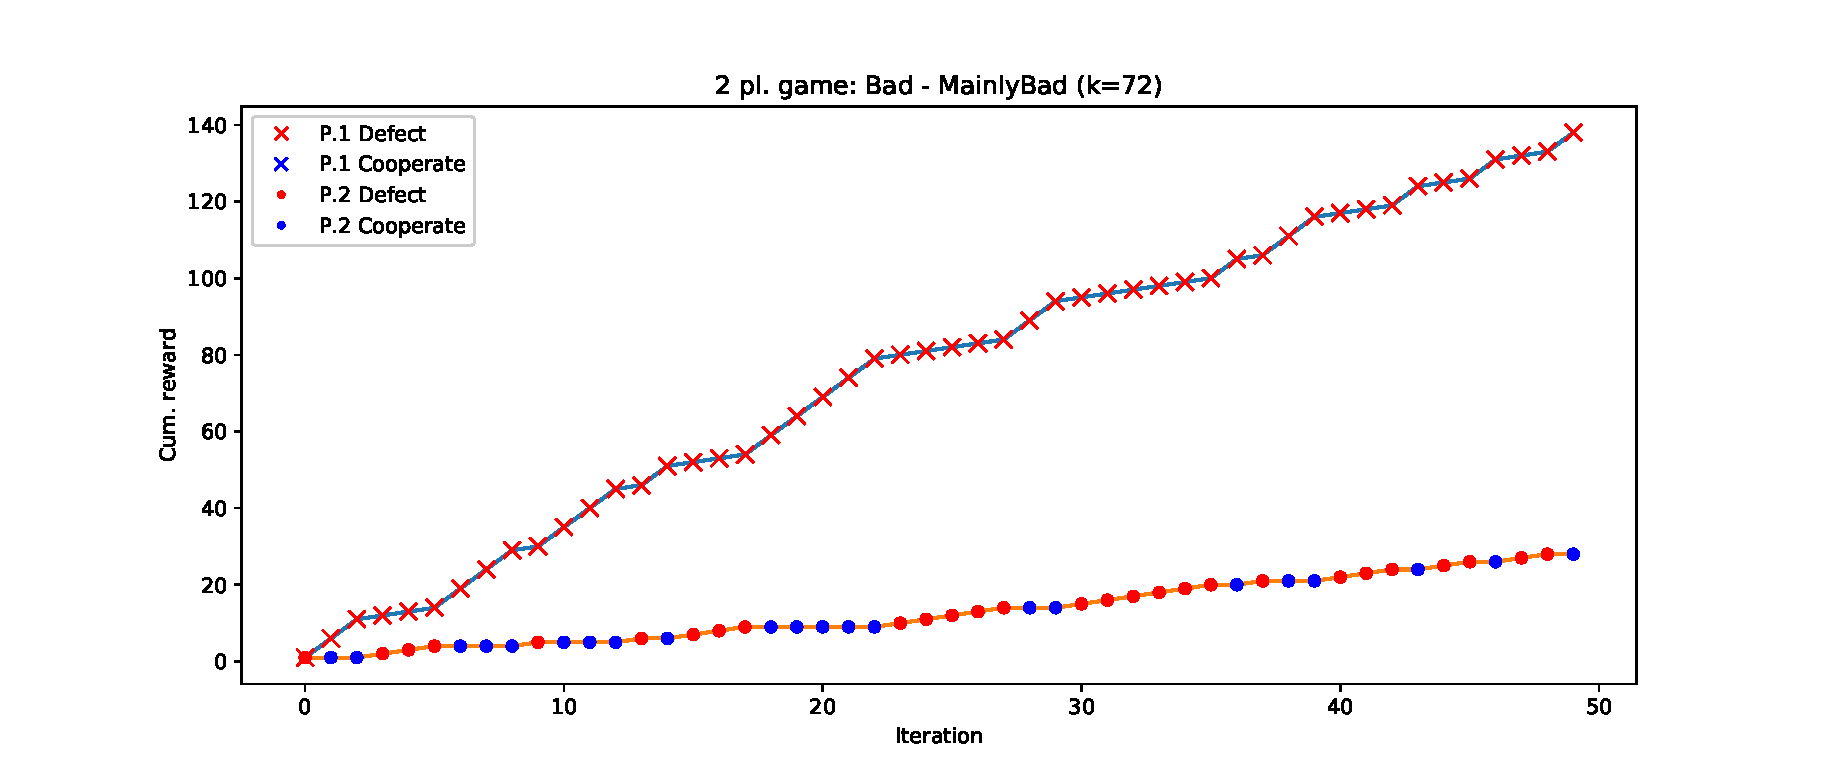
\includegraphics[width=.9\columnwidth]{../img/ipd2p/ipd2p-rewards-Bad-MainlyBad(k=72)}
    \caption{Bad vs Mainly bad}
    \label{fig:badvsmainlybad}
\end{figure}

Taking a closer look, the combination of \textit{Nice} and one between \textit{TfT} or \textit{Nice} leads to better payoffs at the end of the runs as in Figures~[\ref{fig:tftvsindiff},\ref{fig:nicevsnice},\ref{fig:nicevstft}]. The underlying idea is that both players are getting the highest reward, not just one of them, and these choices are cumulatively better, compared to the \textit{Bad}-\textit{Nice} combination.

\begin{figure}[!ht]
    \centering
    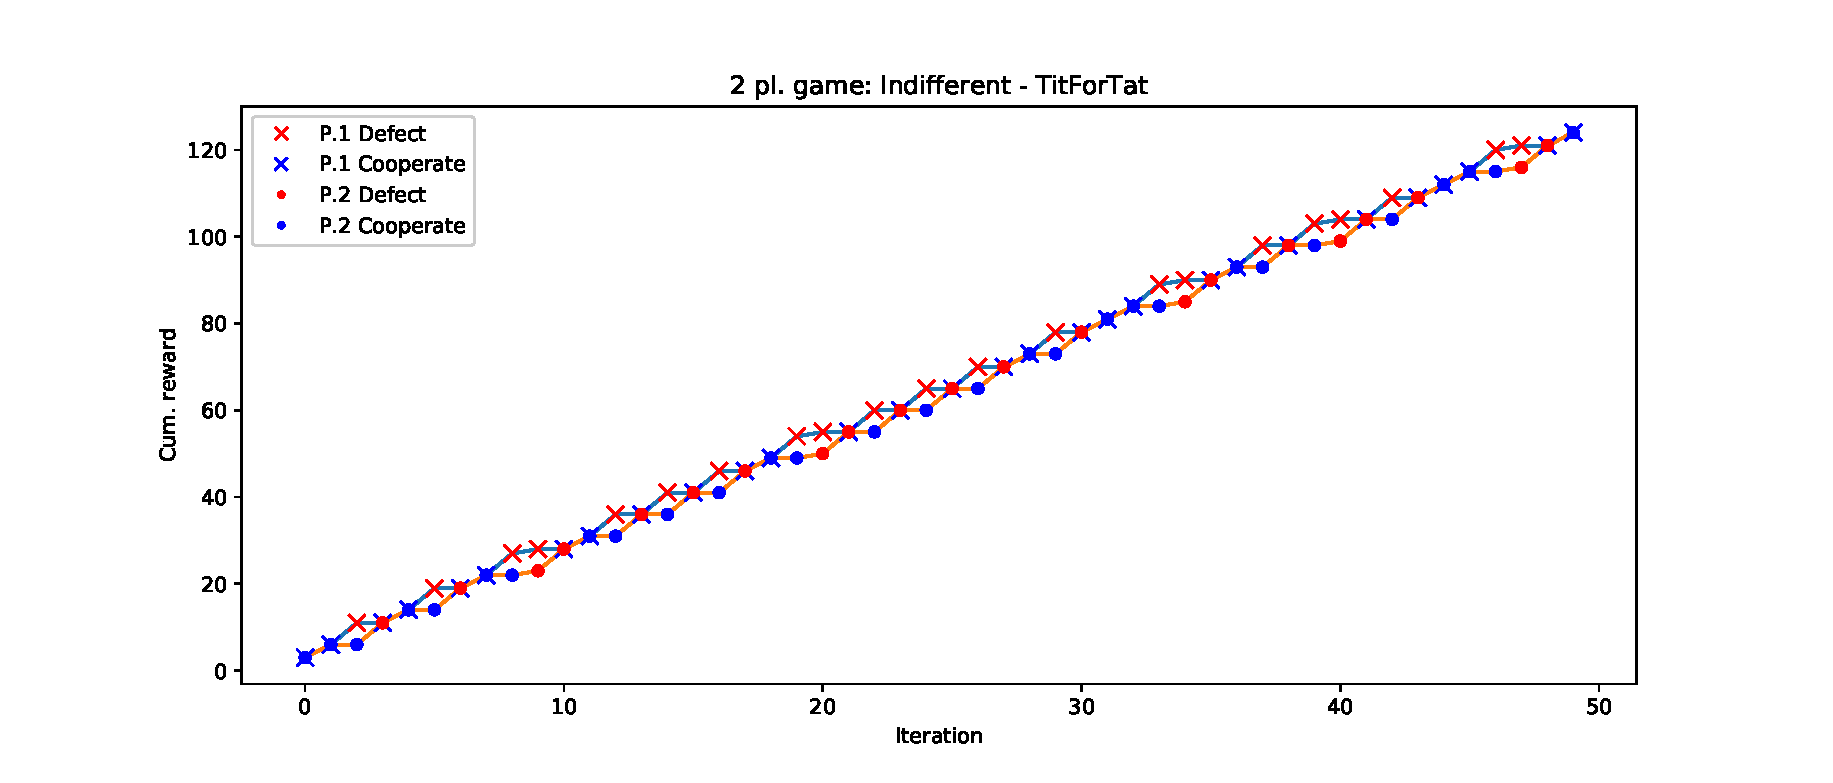
\includegraphics[width=.9\columnwidth]{../img/ipd2p/ipd2p-rewards-Indifferent-TitForTat}
    \caption{TfT vs Indifferent}
    \label{fig:tftvsindiff}
\end{figure}

\begin{figure}[!ht]
    \centering
    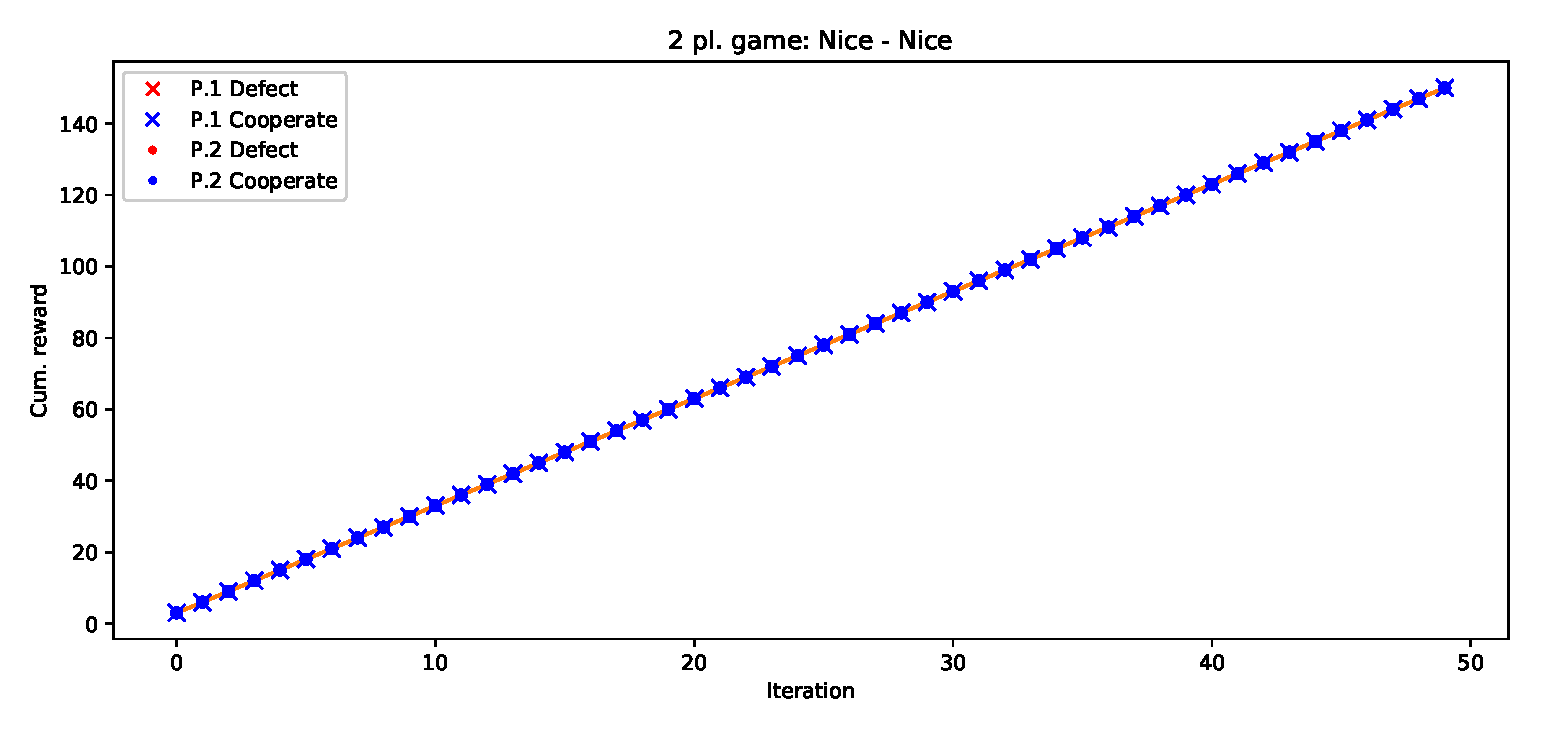
\includegraphics[width=.9\columnwidth]{../img/ipd2p/ipd2p-rewards-Nice-Nice}
    \caption{Nice vs Nice}
    \label{fig:nicevsnice}
\end{figure}

\begin{figure}[!ht]
    \centering
    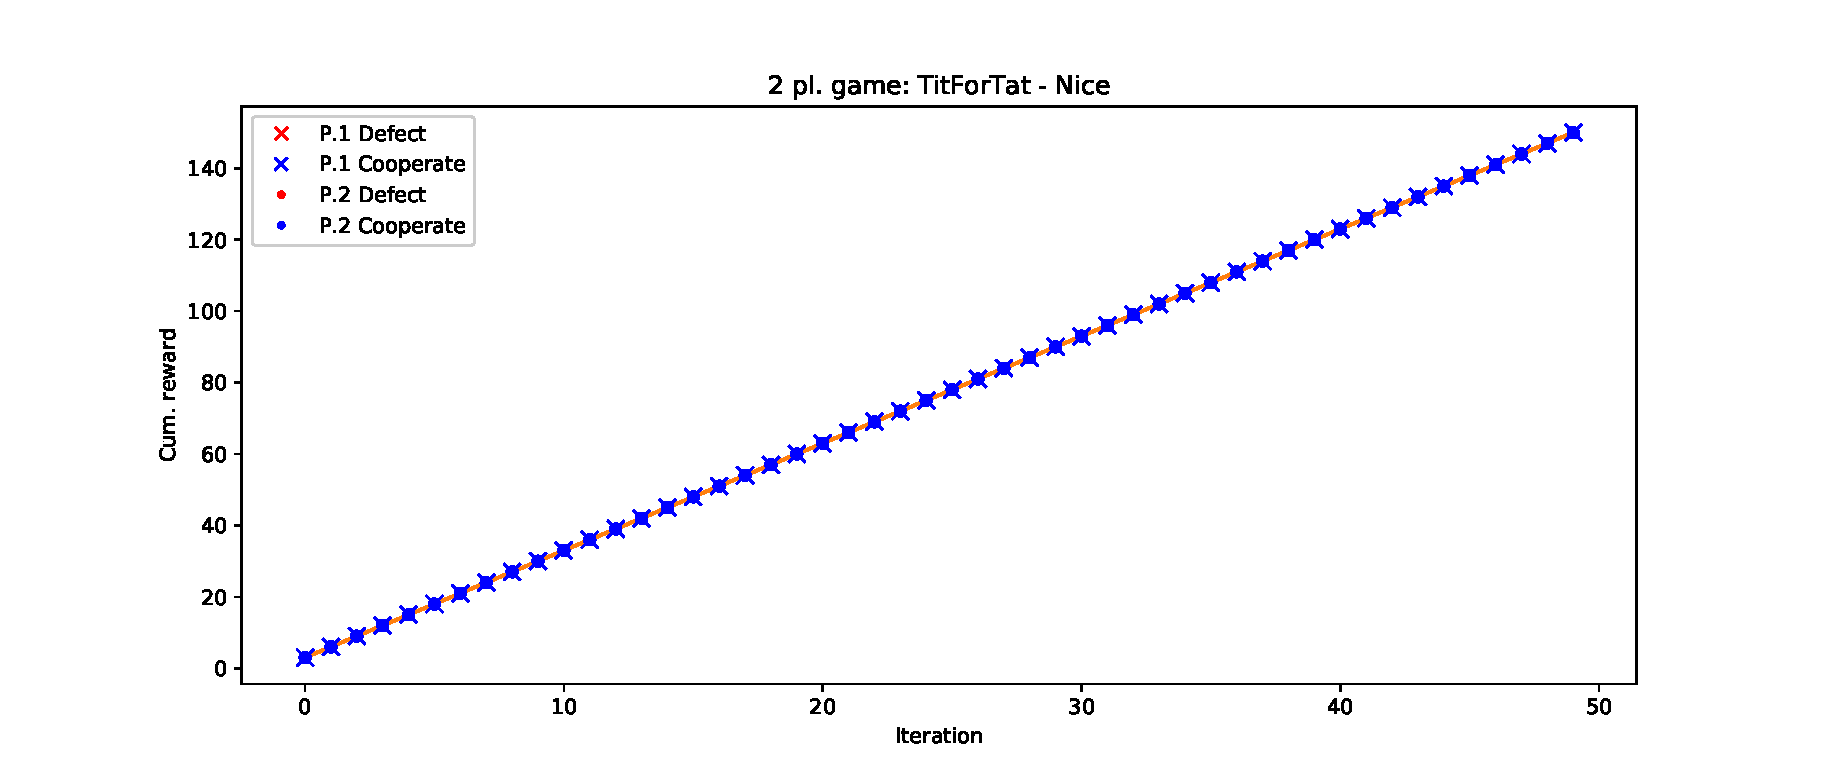
\includegraphics[width=.9\columnwidth]{../img/ipd2p/ipd2p-rewards-TitForTat-Nice}
    \caption{Nice vs TfT}
    \label{fig:nicevstft}
\end{figure}

\begin{figure}[!ht]
    \centering
    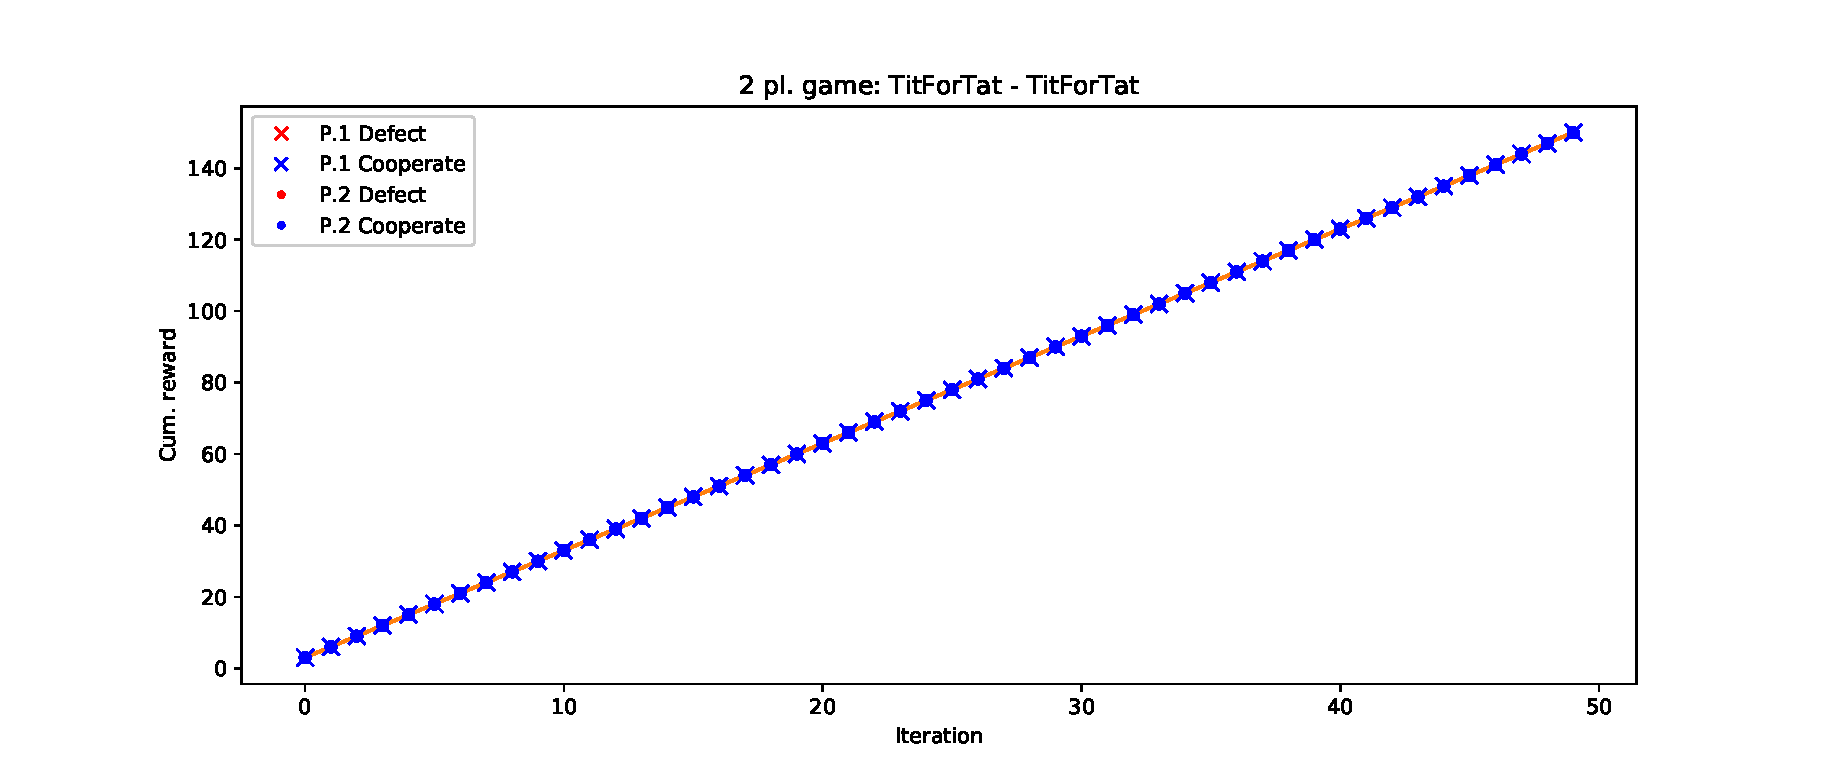
\includegraphics[width=.9\columnwidth]{../img/ipd2p/ipd2p-rewards-TitForTat-TitForTat}
    \caption{TfT vs TfT}
    \label{fig:tftvstft}
\end{figure}

The \textit{TfT} strategy is interesting, because \textit{TfT} leads to almost the same cumulative reward as the opponent, and it is highly adaptive, even if it is fast-forgiving when it plays against a mainly bad strategy. In other words, \textit{TfT} is robust because it never defects first and never takes advantage for more than one iteration at a time.~\cite{fogelEvolvingBehaviors}

In addition to these considerations, simulations were performed multiple times to get insights of the mean and variance of the rewards ruling these games. It is obvious that the static strategies (as the \textit{Nice-Nice}, \autoref{fig:boxnn}), or the non-triggering ones, or the ones without variations have a constant mean and $0$ std. On the other hand, it is interesting to notice that random strategies have a non-null variance, as shown in \textit{Mainly Bad-TitForTat}, \autoref{fig:boxmbvtft}. However, this does not imply that \textit{TitForTat} could ever win against such a strategy, it is only pointing out that there is a variation on subsequent runs based on the randomness of at least one of the two players: the \textit{TfT} strategy is a reactive strategy so it will be always ``late'', meaning that a player applying it will always have the same points of the opponent at the end of the game. There may be particular cases where a Mainly Nice player may defect a Mainly Bad opponent but these are just outliers in the overall simulation.

\begin{figure}[!ht]
    \centering
    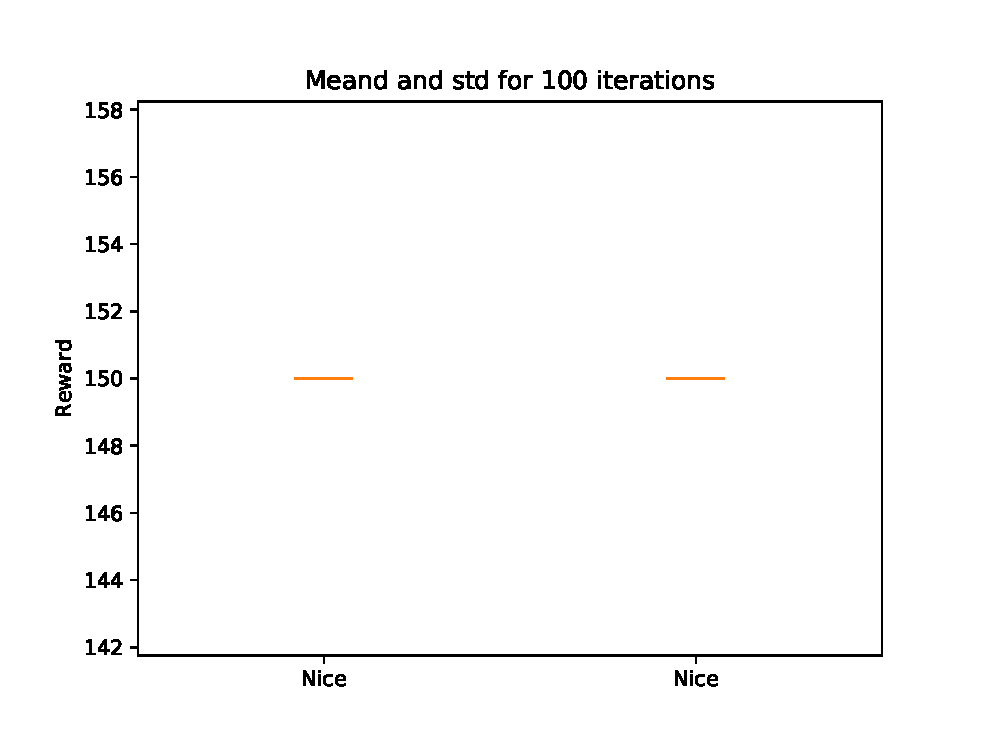
\includegraphics[width=.7\columnwidth]{../img/ipd2p/ipd2p-boxplot-Nice-Nice}
    \caption{Nice vs Nice}
    \label{fig:boxnn}
\end{figure}

\begin{figure}[!ht]
    \centering
    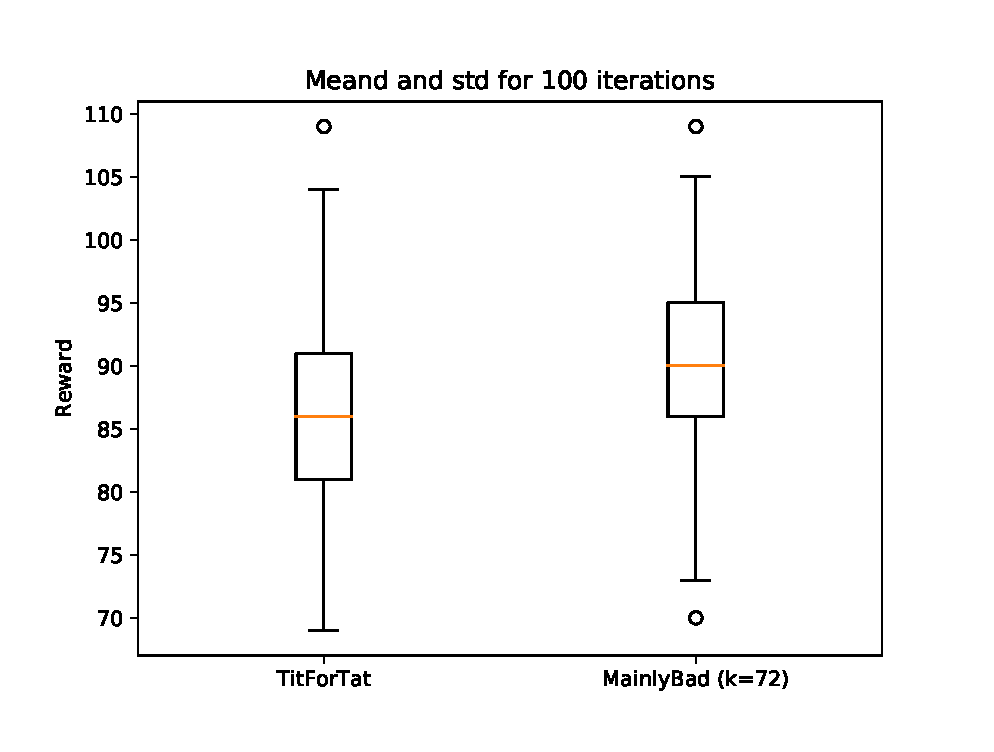
\includegraphics[width=.7\columnwidth]{../img/ipd2p/ipd2p-boxplot-TitForTat-MainlyBad(k=72)}
    \caption{TfT vs Mainly Bad}
    \label{fig:boxmbvtft}
\end{figure}

Moreover, it can be seen that the only strategies that reach $0$ as a final payoff are the \textit{Nice} ones, while the \textit{TfT, Tf2T, GrT, Bad} have a higher minimum value.

It is impossible to make the optimal score against all strategies. The most intuitive reason is a consequence of the first move: to play optimally against a \textit{Bad} guy, it is necessary to defect at the first round, and, as already discussed, to play optimally against \textit{GrT} (or equivalently \textit{TfT}), it is necessary to cooperate until the last round where you should defect.~\cite{mathieu2017}
But the number of rounds is unknown to the players and they should know in advance the type of opponent: this would enable them to adapt their strategy, but is not allowed by the rules of the game. 

Finally, two additional metrics have been introduced: \textit{yield} and \textit{achieve}. 
Being $p$ and $q$ two players, each with a given strategy, the metrics can be expressed as
$$
\mathrm{yield}(p) = \frac{\mathrm{points}(p)}{\mathrm{optimal\_pts}(q)} \quad
\mathrm{achieve}(p) = \frac{\mathrm{points}(p)}{\mathrm{hoped\_pts}(p,q)}
$$
where $\mathrm{points}(p)$ is the number of points at the end of the round,
$\mathrm{optimal\_pts}(p)$ is the maximum that $p$ could achieve if he knew $q$'s moves in advance, and
$\mathrm{hoped\_pts}(p,q)$ is the best result player $p$ can achieve in the optimal scenario or, in other words, supposing that the opponent $q$ would respond in a way such that $p$ could maximize his payoff.
\textit{Yield} represents how well the player has performed against its opponent with respect to the maximum that he could get if he knew its opponent's moves in advance, while \textit{achieve} represents how far the player is with respect to its best expectation.

The following considerations arise on the grounds of \autoref{tab:ipd2p}.
The \textit{yield} metric backs up our claim that \textit{Bad} is the only win-always strategy as it is the only one that gives a stunning $100\%$ for all the matches playing a perfect move against every opponent, a result that can also be seen in \autoref{tab:ipd2pavg}. In other words, a player using this strategy does not need to know in advance which strategy the opponent is adopting. Moreover, this metric points out how \textit{TfT, Tf2T, GrT} strategies are more resilient, namely, they respond well to strategies in that a player does not reach its maximum achievable points, but performs well irrespective of the opponents' strategy. In particular, \textit{GrT} reaches scores over $90\%$ even against \textit{(Mainly) Bad} players.

The \textit{achieve} column is a coupled metric that takes into account both players. We notice once again that, ruling out the same-strategy couples, \textit{TfT, Tf2T} and \textit{GrT} strategies achieve results (almost) always comparable with the opponents, meaning that they are at least as good as them.

On the contrary, taking the averages of these two metrics with respect to all the subsequent matches, it can be seen how the only strategies that achieve high performance on both are the \textit{Tf(2)T} and \textit{GrT}, meaning that even if they do not win every time, they achieve pretty high payoffs.
On the long run, on the basis of these numbers, the conclusion is that these the strategies would emerge since yielding the maximum possible payoff does not imply achieving high overall results.

More insights about this part, including the complete collection of the generated pictures, can be found in the repository and in both \autoref{tab:ipd2p} and \autoref{tab:ipd2pavg}, where collected statistics are presented.

\section{Multiple players IPD - Round-robin scheme} \label{s:IPDMP}
The IPD with \textit{round-robin} (RR) scheme, used to match-up the opponents, consists in a number of players, with multiple strategies, not necessarily different, with each player playing once against each other for a fixed \texttt{NUM\_ITER} of times. This value is set by default to $50$ in simulations but can be changed with a parameter when launching the program.

Each player chooses its fixed strategy at the beginning of the tournament and holds it throughout the course of the match without knowing the strategies of the other players.

In short, it is a variation of the previous case, in which multiple players, with possibly different strategies, play in a RR way. The variation consists in the fact that a single player will win the tournament if at the end, he has the highest cumulative payoff.
Since there are $C=N\cdot (N-1)/2$ possible couples of players and $I$ iterations of the game, at the end, the total number of matches will be $C\cdot I$. From the perspective of each single player, the total number of match to attend is simply $I\cdot(N-1)$.

Tournament statistics like points and counts of cooperation and defection moves, along with the percentage of cooperation, are shown in \autoref{tab:ipdmp50}.

As a validation proof, our results have been compared to the ones obtained from the Axelrod Tournament Demo software, \cite{demosw} but this software does not implement all the strategies considered in this work. For example, \textit{GrT} is \textit{Spiteful}, but the software cannot set \textit{Mainly Bad/Good} strategies with a given probability of cooperating for which a \textit{Random} agent is used as a substitute. Thus, slightly different outcomes were foreseen due to this constraint; however, this notwithstanding, the evolution of the tournament is quite similar between the two simulations.
Doing a special simulation with only deterministic strategies leads to the same results, as it can be seen comparing \autoref{tab:ipdmp10stat} and \autoref{fig:ipdmp10statsw} in the \hyperref[s:appendix]{Appendix}.

Throughout our tests, we noticed how the results of the tournament, and of the following study-cases, depend on the initial population and the balance between the amount of ``good'' and ``bad'' players. Changing the population could lead to different results: an insight that is rarely pointed out in literature.

Analyzing the 50 players game as in Figures~[\ref{fig:ipdmp50evo},\ref{fig:ipdmp50boxsingle},\ref{fig:ipdmp50boxfinal}], where a random strategy is assigned to each player, the winning strategy is \textit{GrT}. Just behind it, there is \textit{TfT}, followed by a tight set of \textit{Tf2T}, \textit{(Mainly) Bad}, \textit{Bad} and \textit{Indifferent} strategies. Lastly, \textit{(Mainly) Nice} strategies achieve the lowest scores.

\begin{figure}[!ht]
    \centering
    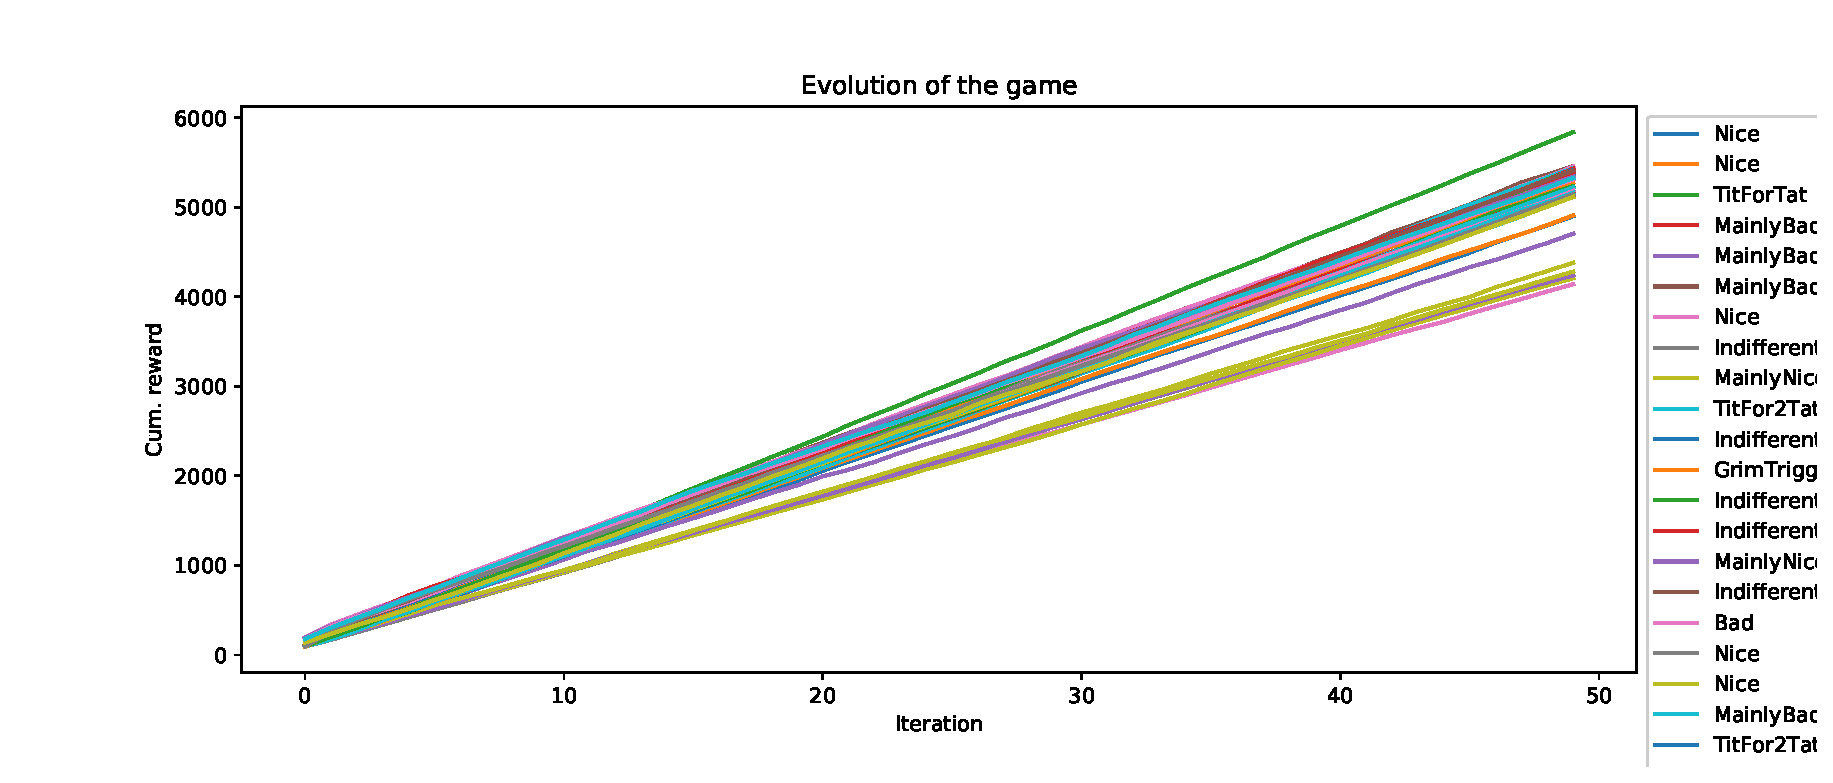
\includegraphics[width=1\columnwidth]{../img/ipdmp/ipdmp-evolution-of-game-50}
    \caption{50 players, evolution of the game}
    \label{fig:ipdmp50evo}
\end{figure}

\begin{figure}[!ht]
    \centering
    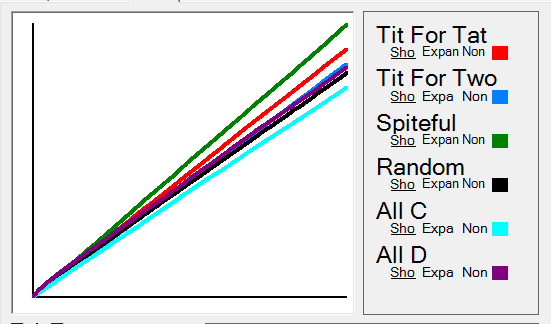
\includegraphics[width=.8\columnwidth]{../img/ipdmp/ipdmp50-plot-det}
    \caption{50 players, evolution -- software results \cite{demosw}}
    \label{fig:ipdmp50evosw}
\end{figure}

\begin{figure}[!ht]
    \centering
    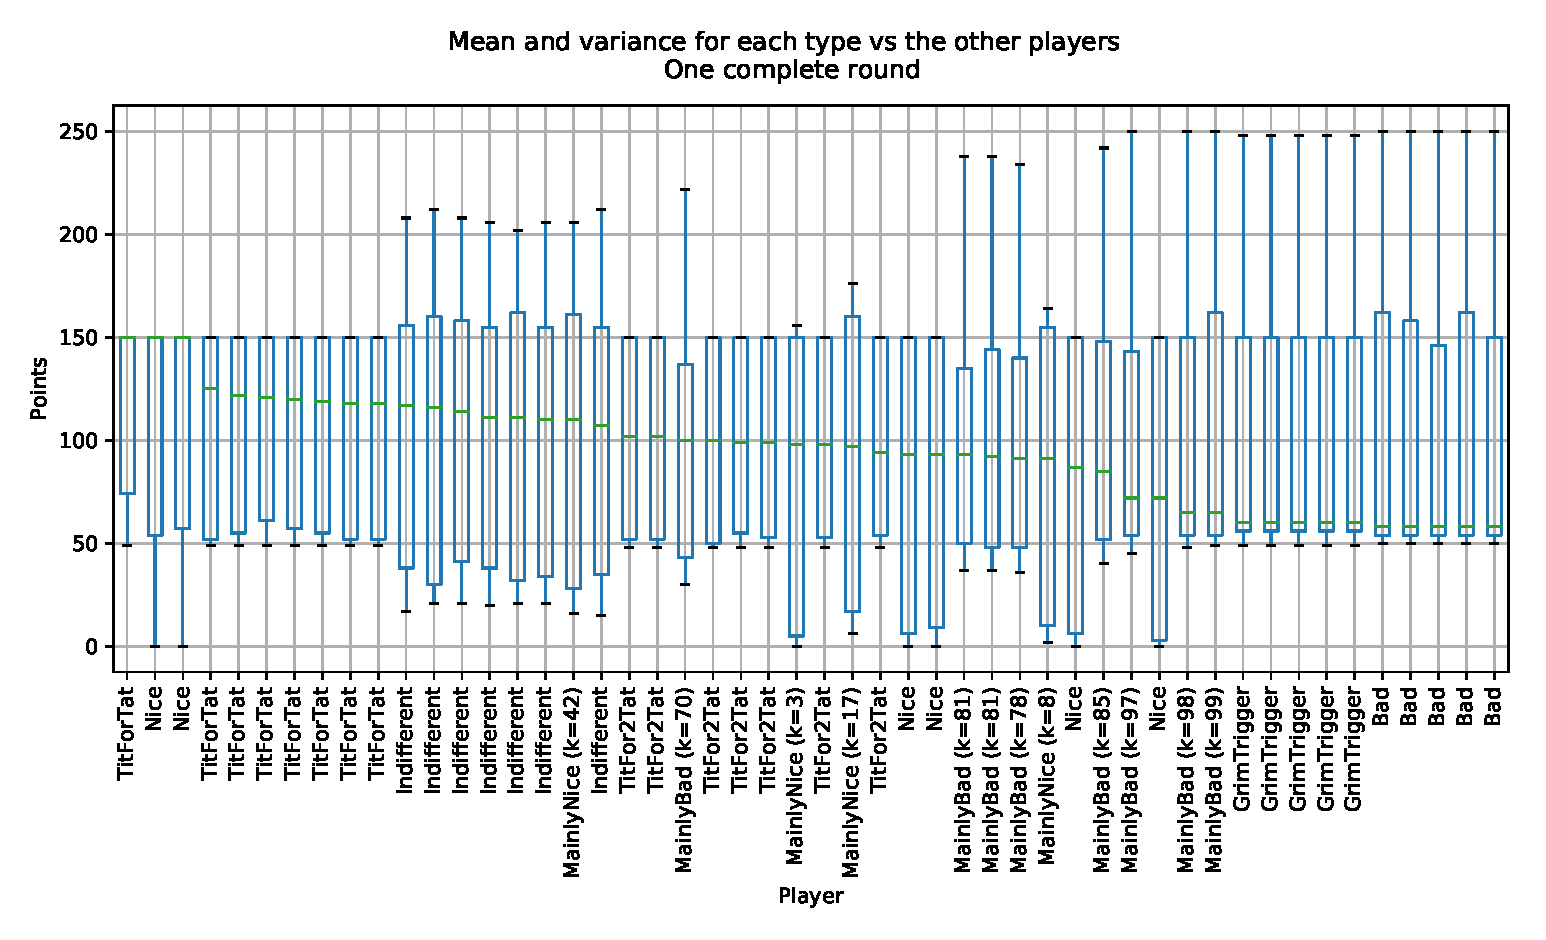
\includegraphics[width=1\columnwidth]{../img/ipdmp/ipdmp-boxplot-single-match-50}
    \caption{50 players, boxplot of a single match}
    \label{fig:ipdmp50boxsingle}
\end{figure}

\begin{figure}[!ht]
    \centering
    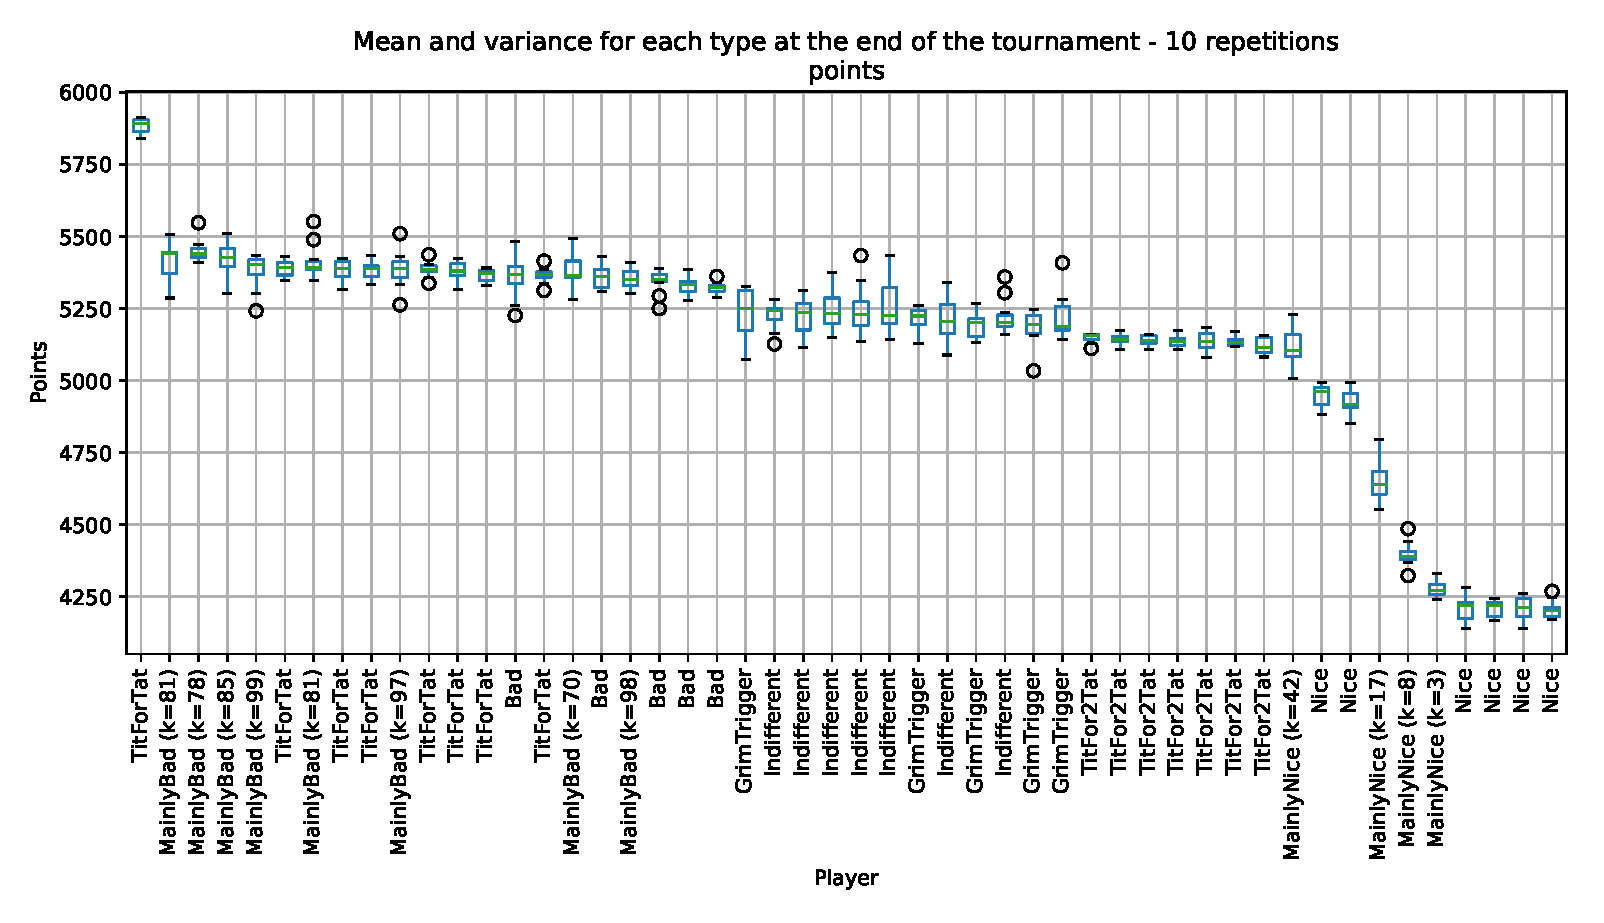
\includegraphics[width=1\columnwidth]{../img/ipdmp/ipdmp-boxplot-final-points-50}
    \caption{50 players, boxplot of the final points}
    \label{fig:ipdmp50boxfinal}
\end{figure}

In a 10 players game, as presented in \autoref{fig:ipdmp10evo}, the best overall strategy is \textit{TfT}. As pointed out previously, \textit{TfT} is a reactive strategy that leads in most of the cases to almost the same reward as the opponent. After several tries, it is found that a ``good'' setup to get this outcome includes more ``nice'' strategies than ``bad'' ones in order to have a \textit{TfT} winner or to defect the ``bad'' players, there should be enough people with strategies having limited power against ``good'' players (so spiteful or reactive ones). This consideration is not common in the literature but in our opinion it is important and worth noticing, although it can be explained by the game's insights. This statement helps to interpret results and assign them the right meaning.

\begin{figure}[!ht]
    \centering
    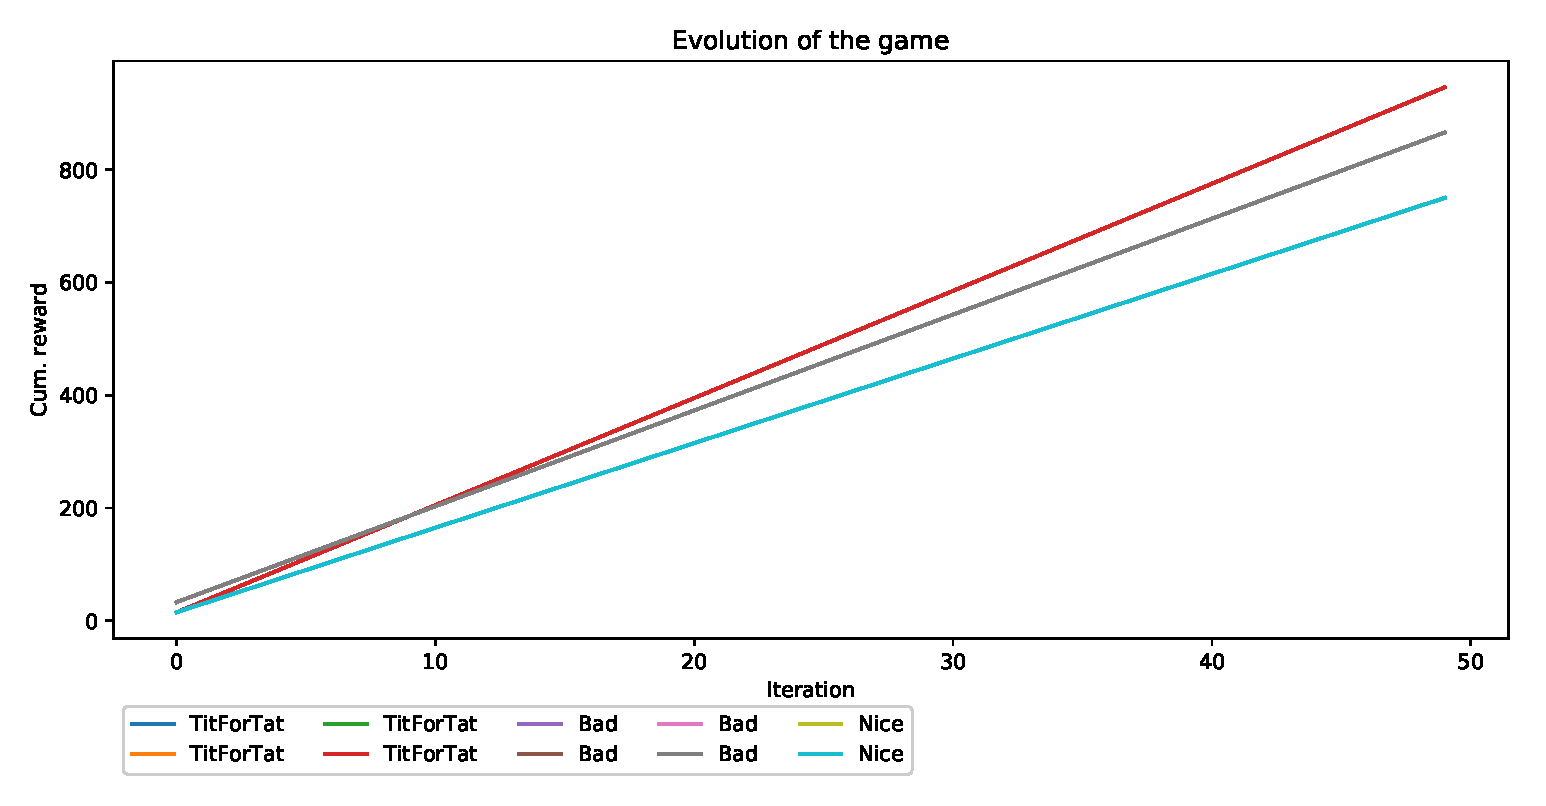
\includegraphics[width=1\columnwidth]{../img/ipdmp/ipdmp-evolution-of-game-10}
    \caption{10 players, evolution of the game}
    \label{fig:ipdmp10evo}
\end{figure}

\begin{figure}[!ht]
    \centering
    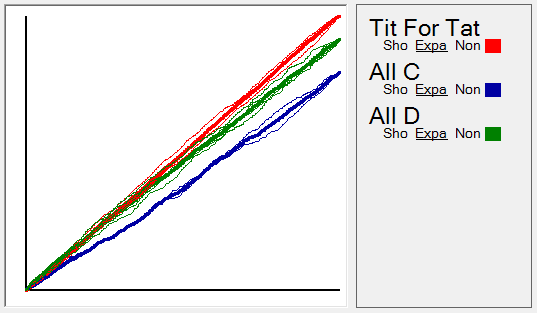
\includegraphics[width=.8\columnwidth]{../img/ipdmp/ipdmp10-plot-det}
    \caption{10 players, evolution -- software results \cite{demosw}}
    \label{fig:ipdmp10evosw}
\end{figure}

Historically \textit{TfT} was considered one of the best strategies to win the tournament since it is one of the best strategies to maximize the score.
This fact was demonstrated in the extensive tests done by Axelrod, thoroughly described in \cite{axelrod1981evolution,axelrod1984evolution} and taken up as a starting point in \cite{mathieu2017}: \textit{TfT}, proposed by Anatol Rapoport, was the winner over all strategies.
However, here it is proven that \textit{TfT} wins only in specific tournaments cases depending on the initial population. Moreover, spiteful strategies like \textit{GrT} seem to get the maximum in heterogeneous and more mixed populations. In any case, both have an extreme behavior even if effective in our testbed. Possible advances can be introduced by taking into account more than the last one or two moves, allowing for more intricate and complex strategies.~\cite{mathieu2017}

In each tournament, some variations of the results can be seen by repeating the simulation multiple times with the same initial population and generating boxplots; since random strategies have been introduced, the result of a one-shot complete game may differ with respect to the average results. These are rare cases that ought to be considered as outliers. Moreover, running simulations with different strategies or with a different initial population (i.e. 20 or 30 players, or by changing the seed), obtained results can be different, especially since the balance between the number of \textit{(Mainly) Bad} and \textit{(Mainly) Nice} guys changes from the previously analyzed scenarios. The results of the tournaments are not predictable without knowing the initial population but this is an information available only to external observers and \textit{not} to the actual players. 

The results are backed also by \textit{achieve} and \textit{yield} metrics that do not change much with respect to ``A vs B'' games.
It can be easily noticed how it is the combination of the two that ``matters'', rather than either of them alone, although obviously players which have an higher \textit{achieve} value are usually in the ``winner'' part of the chart.

\section{Repeated multiple players IPD} \label{s:rIPDMP}
The previously defined MPIPD tournament is now iterated many times and the population changes based on the results obtained in the previous round: the scheme is denoted as a \textit{Repeated MPIPD}~(rMPIPD).

Two main separated scenarios have been developed to study the behavior, the evolution of the populations and the convergence speed by simulations: static and increasing populations (with three separated sub-cases). A population is said to be converged in our simulations if more than $3/4$ of it have the same strategy type at the end of a complete round. The basic rules are the same as pointed out in the previous sections (\textit{common knowledge},  etc.).

\subsection{Static Population} \label{ss:rIPDMPc}
In this case, the number of players is fixed. Each player implements a strategy choosing it with equal probability from the strategies set. At the end of each round, the population is sorted with respect to the cumulative payoff and a fixed percentage $x$ ($30\%$ is the default in our simulations) as of the beginning of the list is ``doubled'', so that for each player in this subset, another player with the same strategy is added to the population. Likewise, the players in the last $x\%$ of the chart are then removed from the game, regardless of their strategies. In this way, the total number of players is ensured to be static and then the convergence of the population through consecutive rounds can be studied. After this step, the scores are zeroed and the tournament can restart.

If convergence is not reached after a maximum number of repetitions, execution of the program is stopped.
This method is similar to that used by Axelrod in his tests~\cite[\S 2.6]{mathieu2017}~\cite{axelrod1984evolution}.

Figures~[\ref{fig:constR},\ref{fig:constFI},\ref{fig:constLI}] show the evolution of a population of 50 players over some iterations.
Details on the evolution of the population, grouped by strategy type, are presented in \autoref{tab:ripdmp-const}.
It can be easily observed how the \textit{GrT} and \textit{TfT} strategies very quickly outpace the others: in just two iterations, they represent almost half of the population, with a predominance of \textit{TfT} players. At the fifth iteration, we can see that \textit{GrT} takes the lead but, as previously stated, results depend on the initial population: for example, by fixing the seed to $24$ as in \autoref{fig:constRseed24} and \autoref{tab:ripdmp-const-24}, it can be pointed out how \textit{TfT} players dominate, while using $1209$ as seed (\autoref{fig:constRseed1209} and \autoref{tab:ripdmp-const-1209}) leads to a final population formed by mostly \textit{Bad} players.

These results add some new insights to the previous results obtained by the simulation of the iterated Prisoner's Dilemma: the \textit{TfT} overwhelms its brother \textit{Tf2T}. Taking the scores into account, we can notice how \textit{GrT} and \textit{TfT} are pretty similar since they do not trigger each other.

\begin{figure}[!ht]
    \centering
    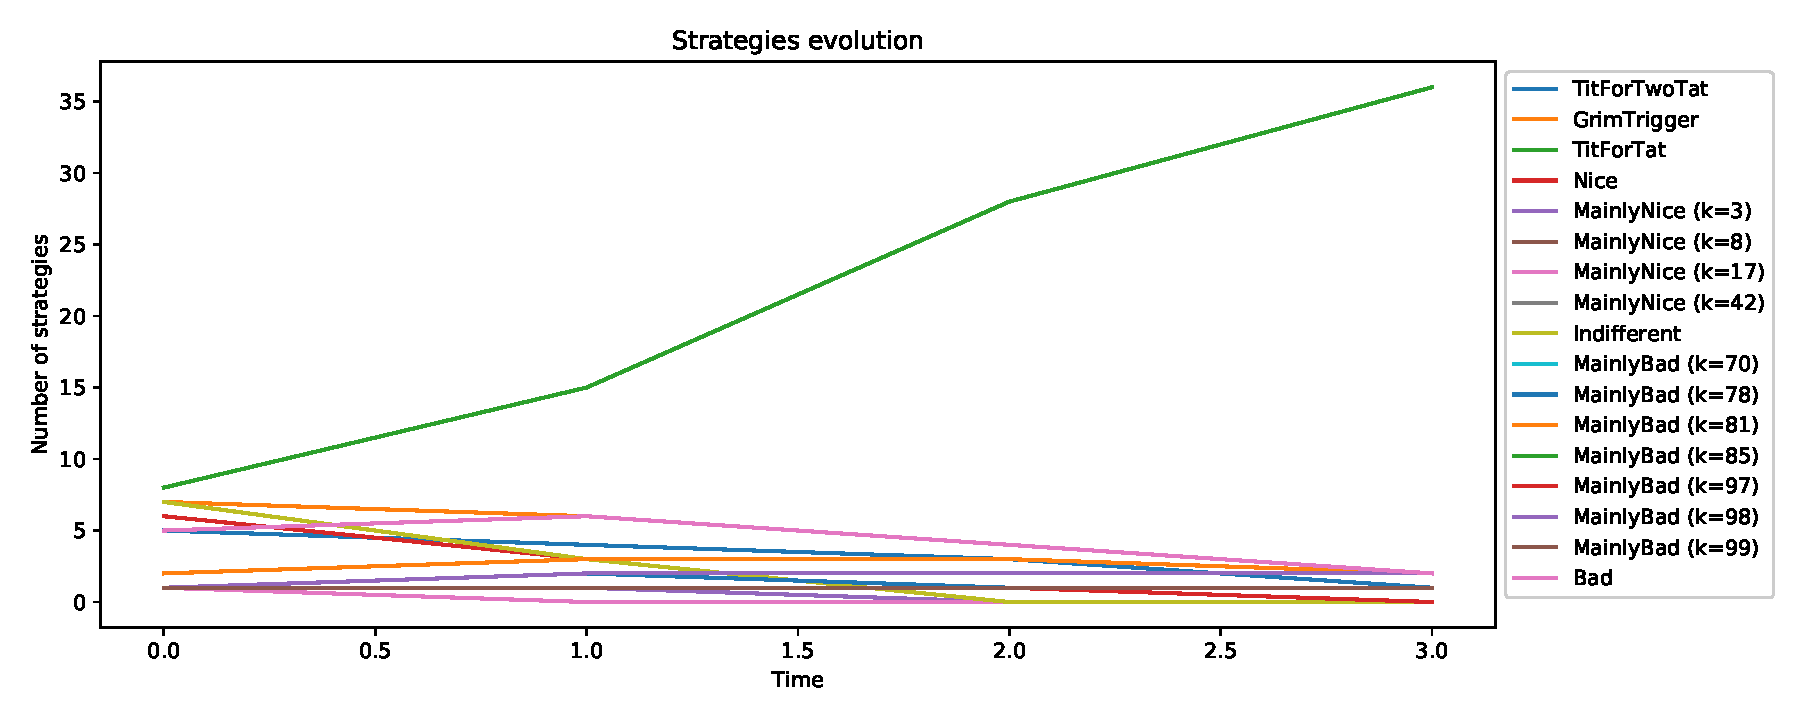
\includegraphics[width=1\columnwidth]{../img/ripdmp-const/ripdmp-evolution-const-pop-50}
    \caption{Evolution of rIPDMP, constant population of 50}
    \label{fig:constR}
\end{figure}

\begin{figure}[!ht]
    \centering
    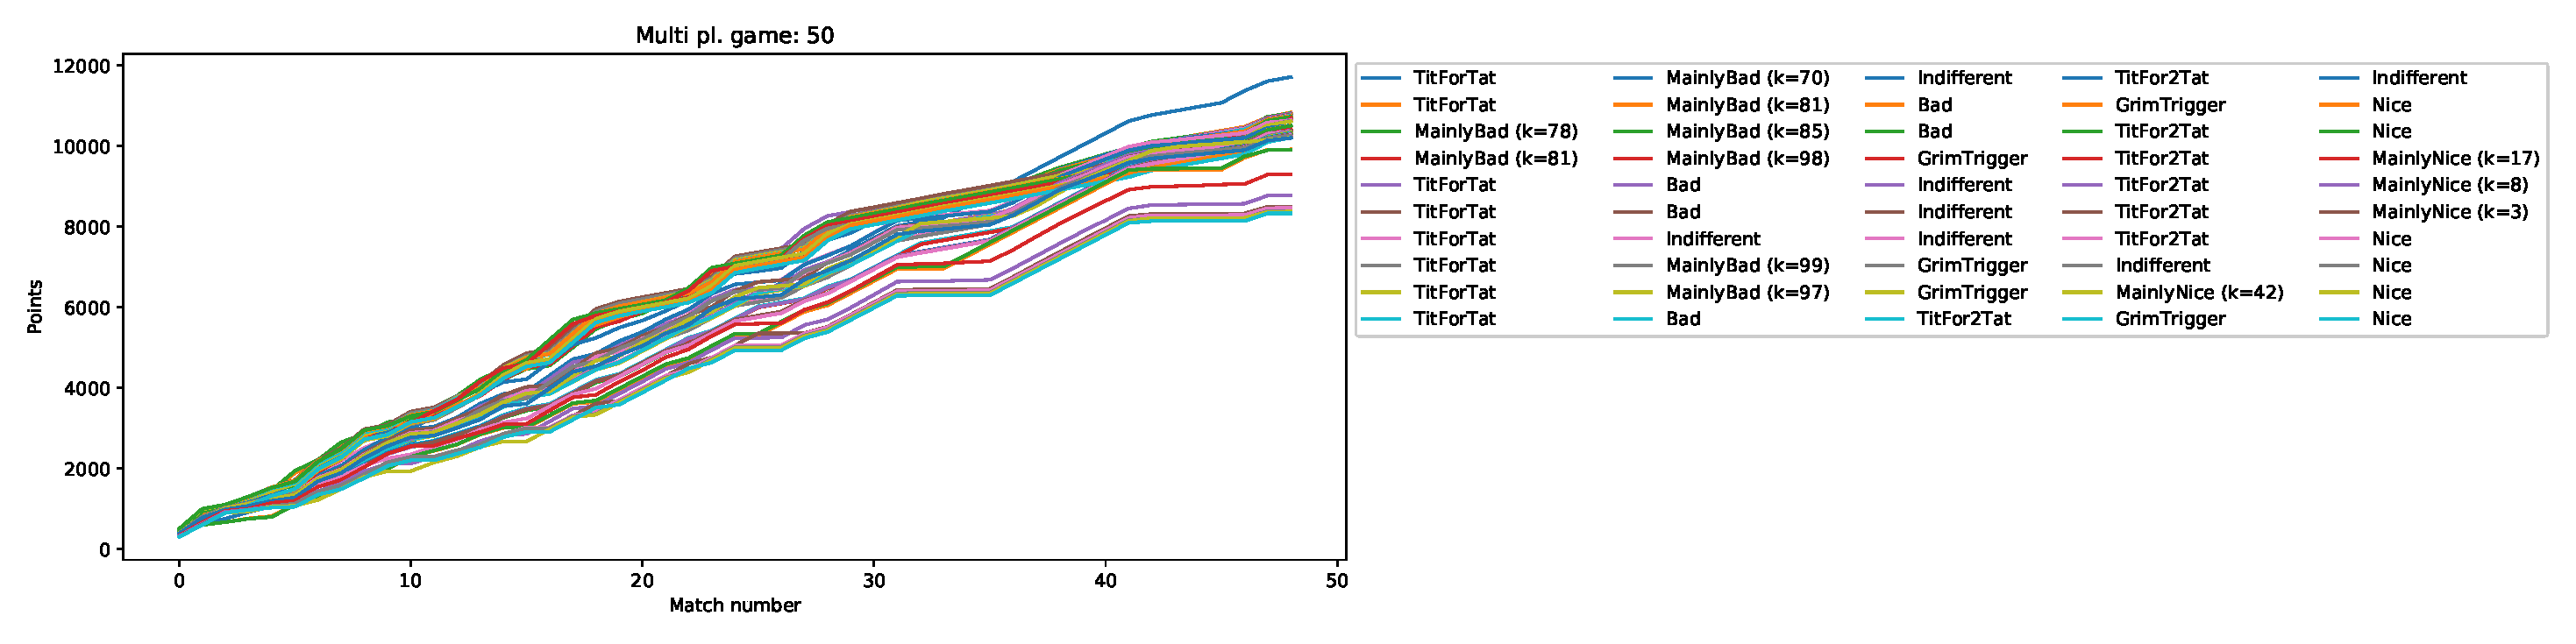
\includegraphics[width=1\columnwidth]{../img/ripdmp-const/ripdmp-scores-const-pop-50-r0}
    \caption{First iteration scores ($it=0$)}
    \label{fig:constFI}
\end{figure}

\begin{figure}[!ht]
    \centering
    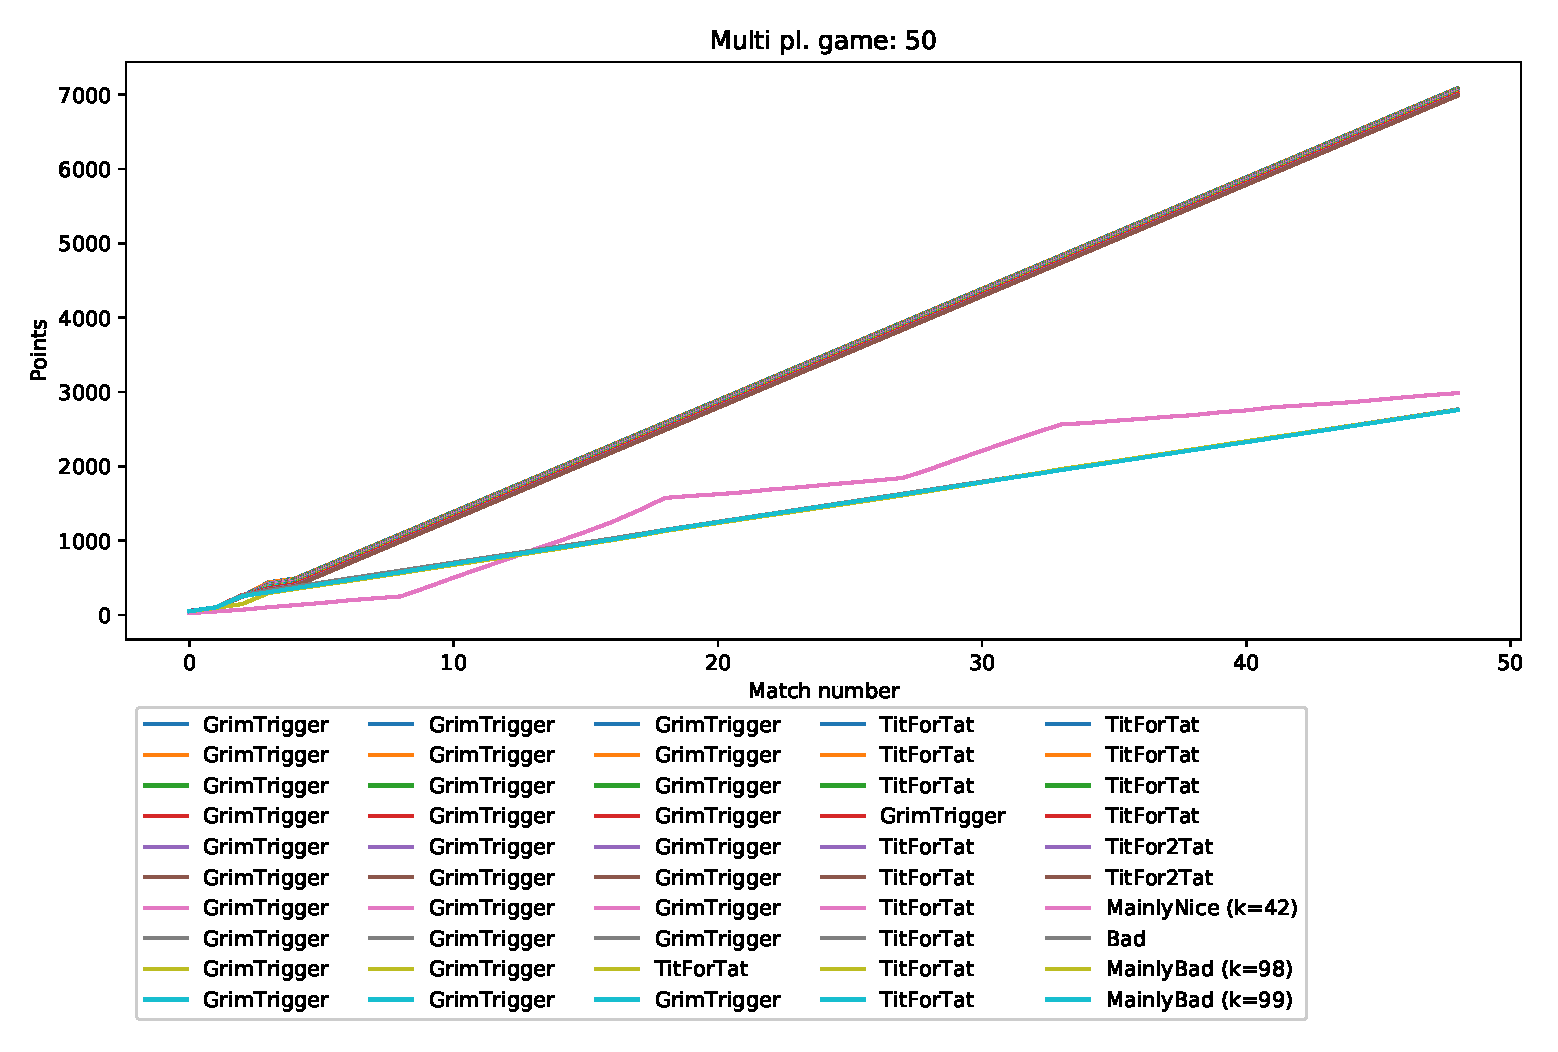
\includegraphics[width=1\columnwidth]{../img/ripdmp-const/ripdmp-scores-const-pop-50-r3}
    \caption{Last iteration scores ($it=4$)}
    \label{fig:constLI}
\end{figure}

\begin{figure}[!ht]
    \centering
    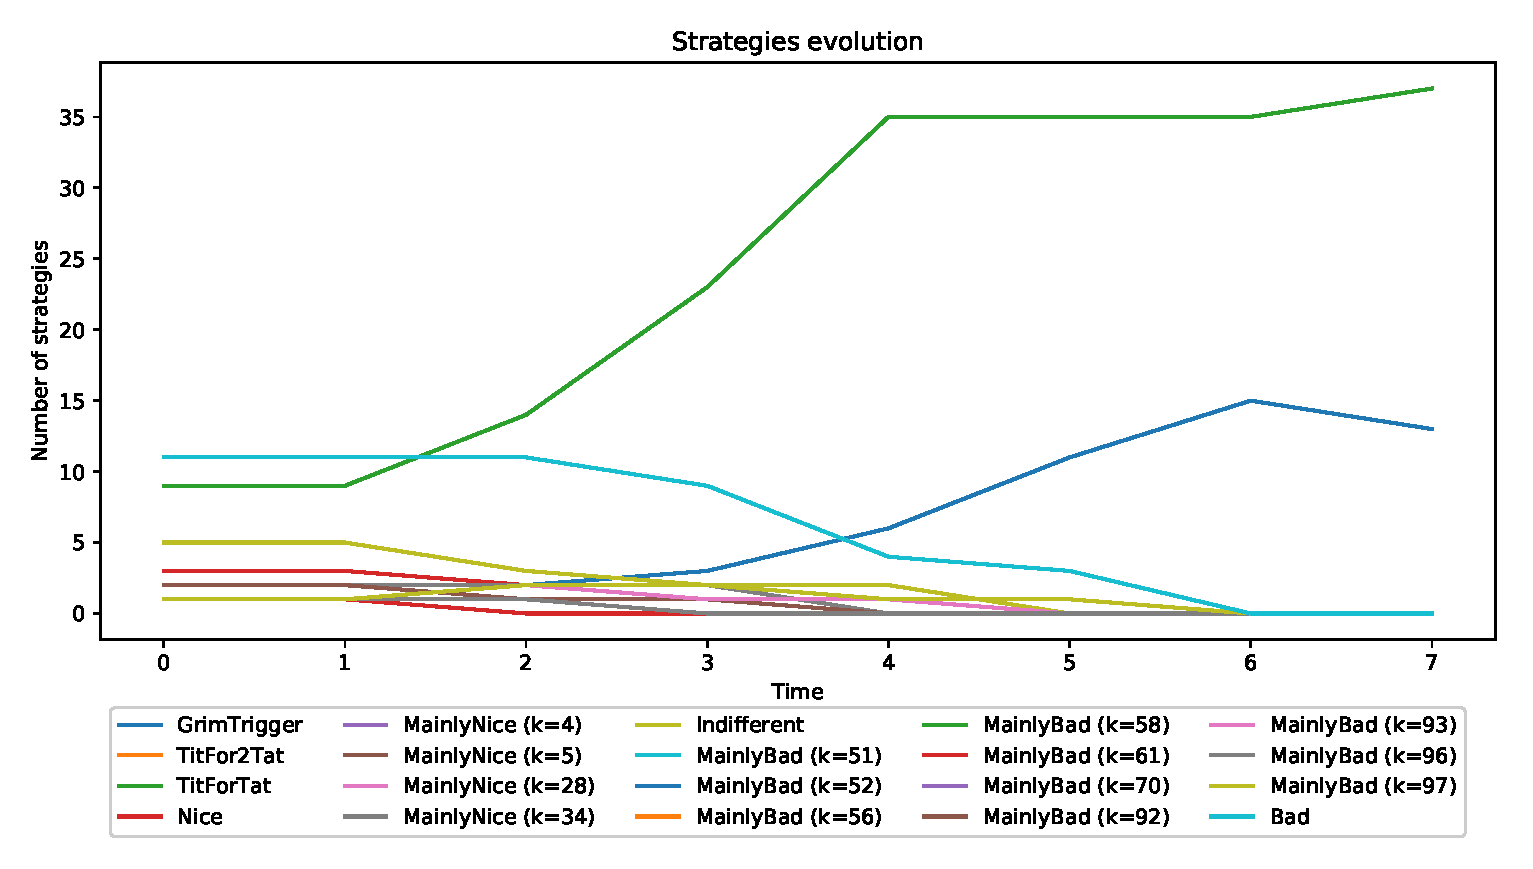
\includegraphics[width=1\columnwidth]{../img/ripdmp-const/seed24/ripdmp-evolution-const-pop-50}
    \caption{Evolution of 50 players, $seed = 24$}
    \label{fig:constRseed24}
\end{figure}

\begin{figure}[!ht]
    \centering
    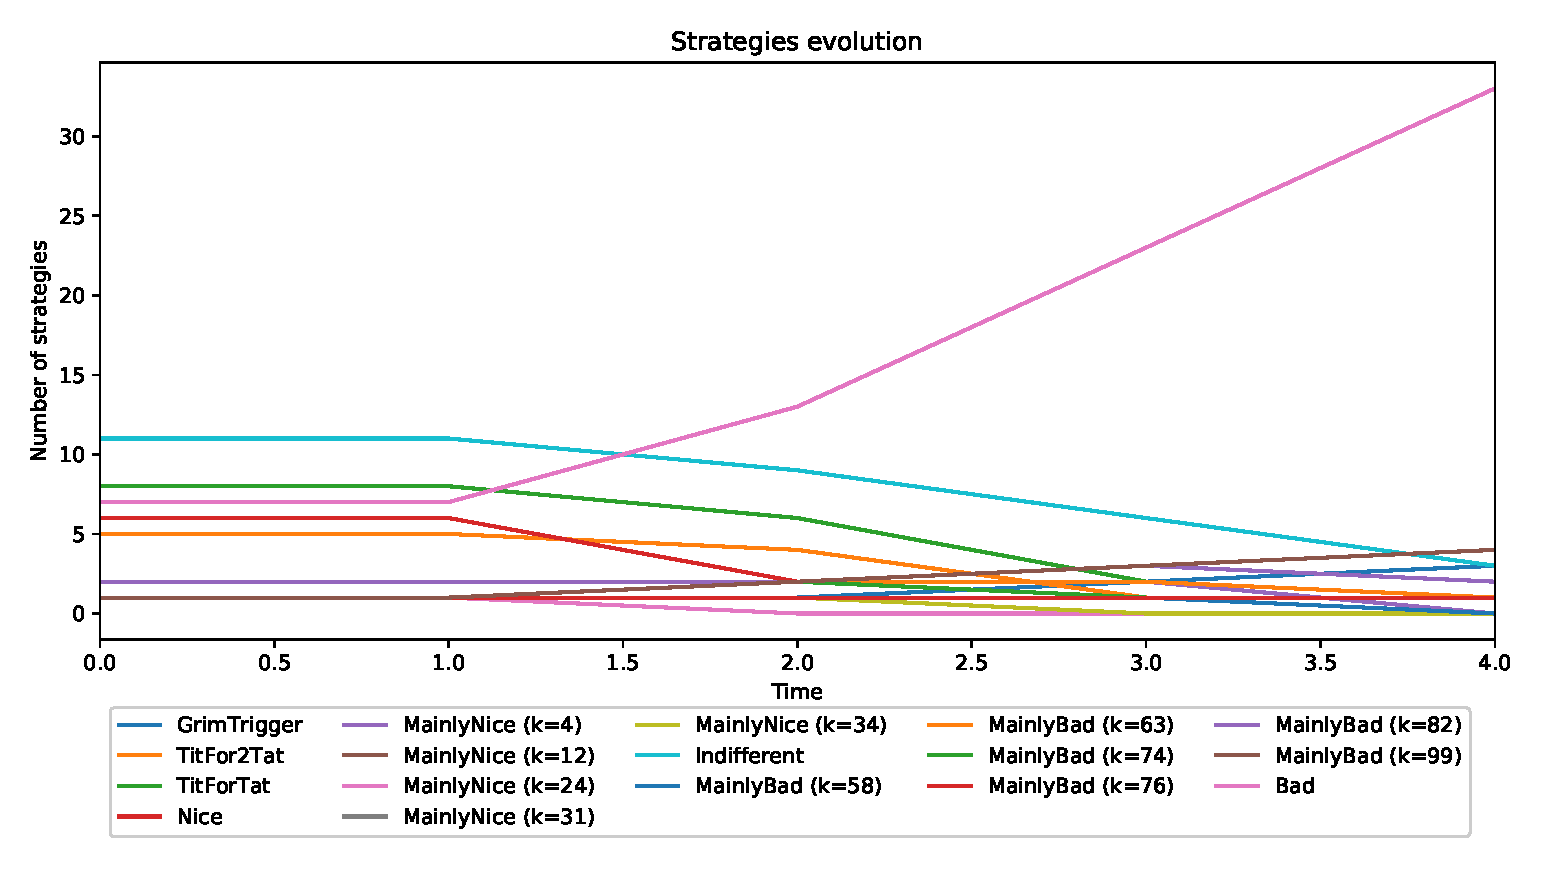
\includegraphics[width=1\columnwidth]{../img/ripdmp-const/seed1209/ripdmp-evolution-const-pop-50}
    \caption{Evolution of 50 players, $seed = 1209$}
    \label{fig:constRseed1209}
\end{figure}

\subsection{Increasing Population} \label{ss:rIPDMPi}
In this case, the number of players (population) is increased at each iteration. Three different ways of adding population between rounds have been implemented; after each round, a player has a certain probability based on his ranking to have a child of the same type:
\begin{enumerate}
    \item The probability is $p(i)=1- i\ /\ num\_players$ where $i$ is the position reached by the player. The winner of the round is indeed doubled, because $p(0)=1$, while the looser is not, as $p(last)=0$.
    For each player, a random number $d$ is drawn, according to a uniform probability distribution, and compared with $p(i)$. If $p(i)$ is greater than $d$ the player is effectively doubled, otherwise not.
    \item The ordered population is split into three sets of equal size $A,B,C$. For each player in the population, a random number $d$ is drawn and its strategy is doubled if:
    \begin{itemize}
        \item $d>0.2$ if the player belongs to $A$
        \item $d>0.5$ if the player belongs to $B$
        \item $d>0.8$ if the player belongs to $C$
    \end{itemize}
    This is an alternative way to promote best strategies, due to the higher probability of being doubled, and obstruct less performing players, whose total number does not increase significantly.
    \item A player's score is defined as its obtained points divided by the maximum obtained score in the whole population. The player's strategy is doubled if a drawn random number is greater than its score.
\end{enumerate}

In our software, the first of the three proposed methods is used by default. Other methods can be set using the \texttt{ALTERNATIVE} variable.

Figures~[\ref{fig:incrR},\ref{fig:incrFI},\ref{fig:incrMI},\ref{fig:incrLI}] show the evolution of a population of 50 players over four iterations using alternative $1$. In this case, convergence is not reached at the fifth iteration, since the population is increasing, but the simulation still shows the same behavior. The \textit{GrT} and \textit{TfT} strategies are getting stronger and stronger. In conclusion, in the future, i.e. evaluating the problem with more iterations, the population will increase with similar behavior and converge to these strategies as in the constant population scenario. Details on the evolution of the population can be found in \autoref{tab:ripdmp-incr}.

Simulation times grow at each iteration since for each player, as we have seen in \autoref{s:IPDMP}, $I\cdot(N'-1)$ rounds are added and $I\cdot(N'-1)\cdot{NUM\_ITER}$ iterations have to be played and the results sorted: this easily explodes. Taking into account the dependence with respect to the initial population, what is suggested from the previous constant population case is preserved also when the population number constraint is relaxed.

\begin{figure}[!ht]
    \centering
    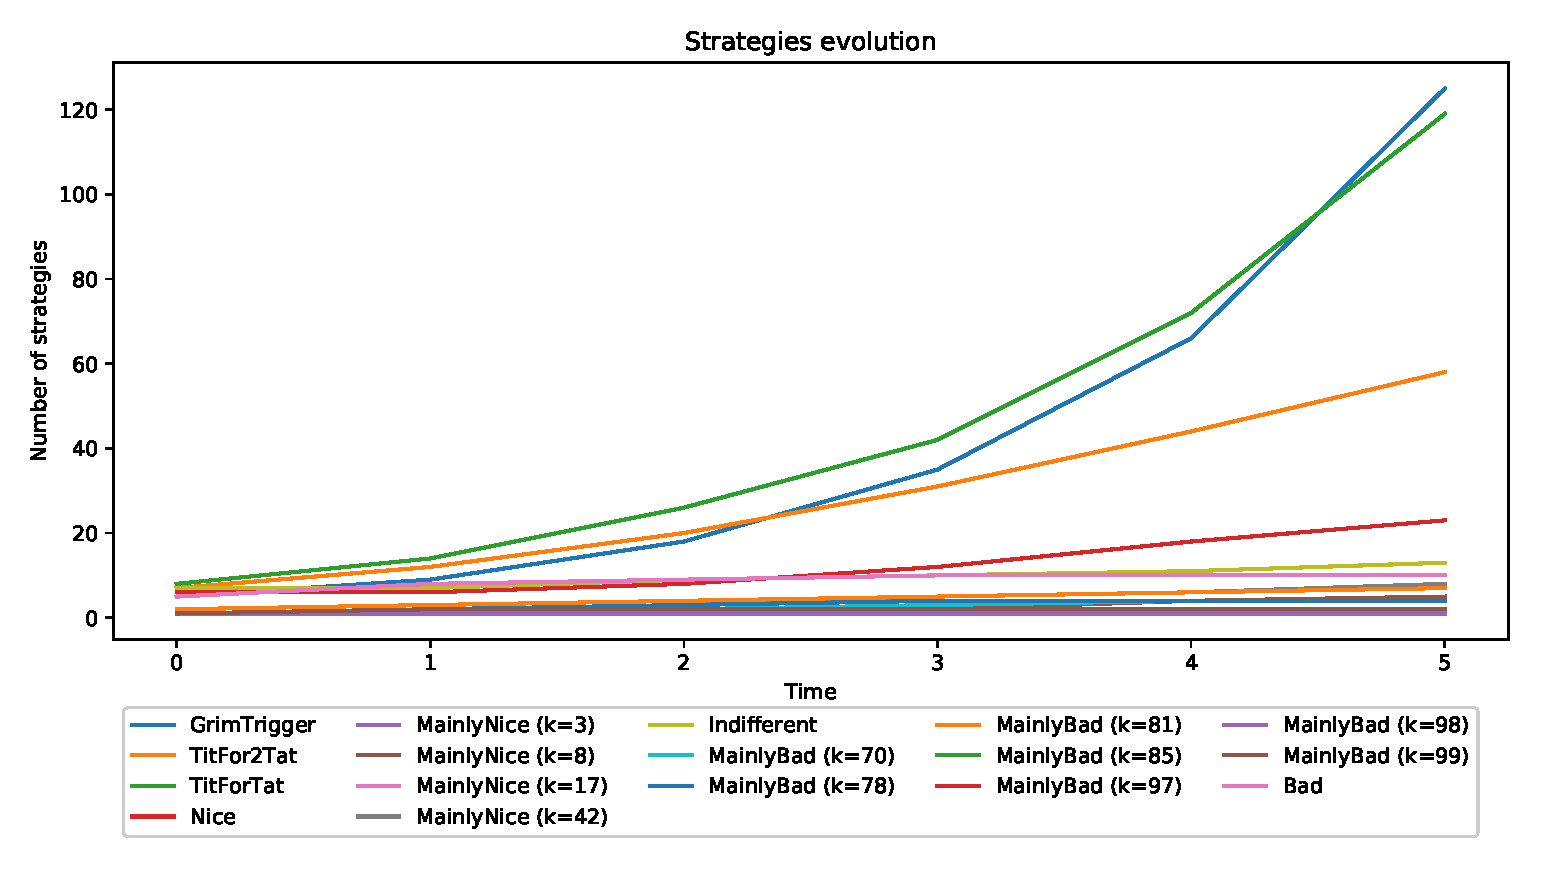
\includegraphics[width=1\columnwidth]{../img/ripdmp-incr/alt1/ripdmp-evolution-increasing-pop-50}
    \caption{Evolution of rIPDMP, increasing population, from 50}
    \label{fig:incrR}
\end{figure}

\begin{figure}[!ht]
    \centering
    \includegraphics[width=1\columnwidth]{../img/ripdmp-incr/alt1/ripdmp-scores-increasing-pop-50-r0}
    \caption{First iteration scores ($it=0$)}
    \label{fig:incrFI}
\end{figure}

\begin{figure}[!ht]
    \centering
    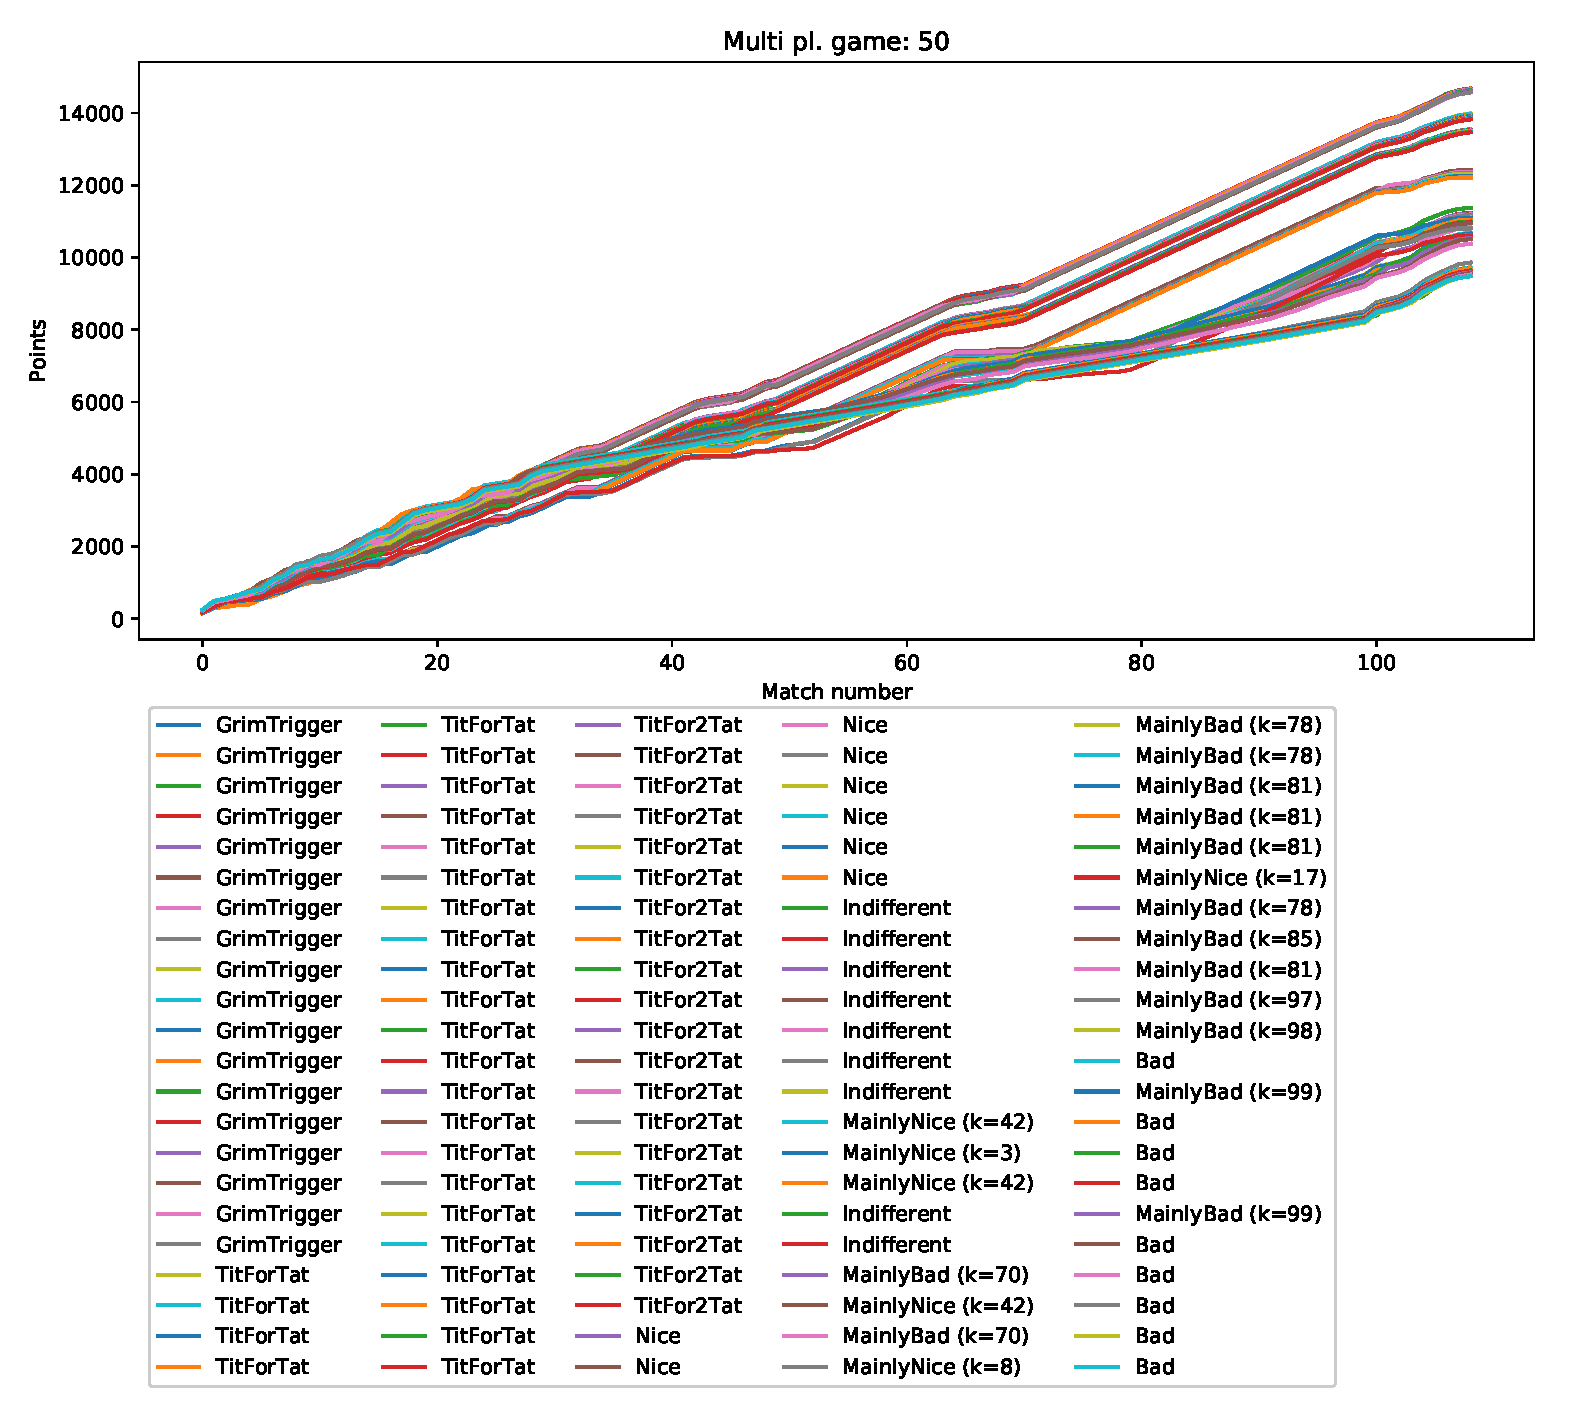
\includegraphics[width=1\columnwidth]{../img/ripdmp-incr/alt1/ripdmp-scores-increasing-pop-50-r2}
    \caption{Middle iteration scores ($it=2$)}
    \label{fig:incrMI}
\end{figure}

\begin{figure}[!ht]
    \centering
    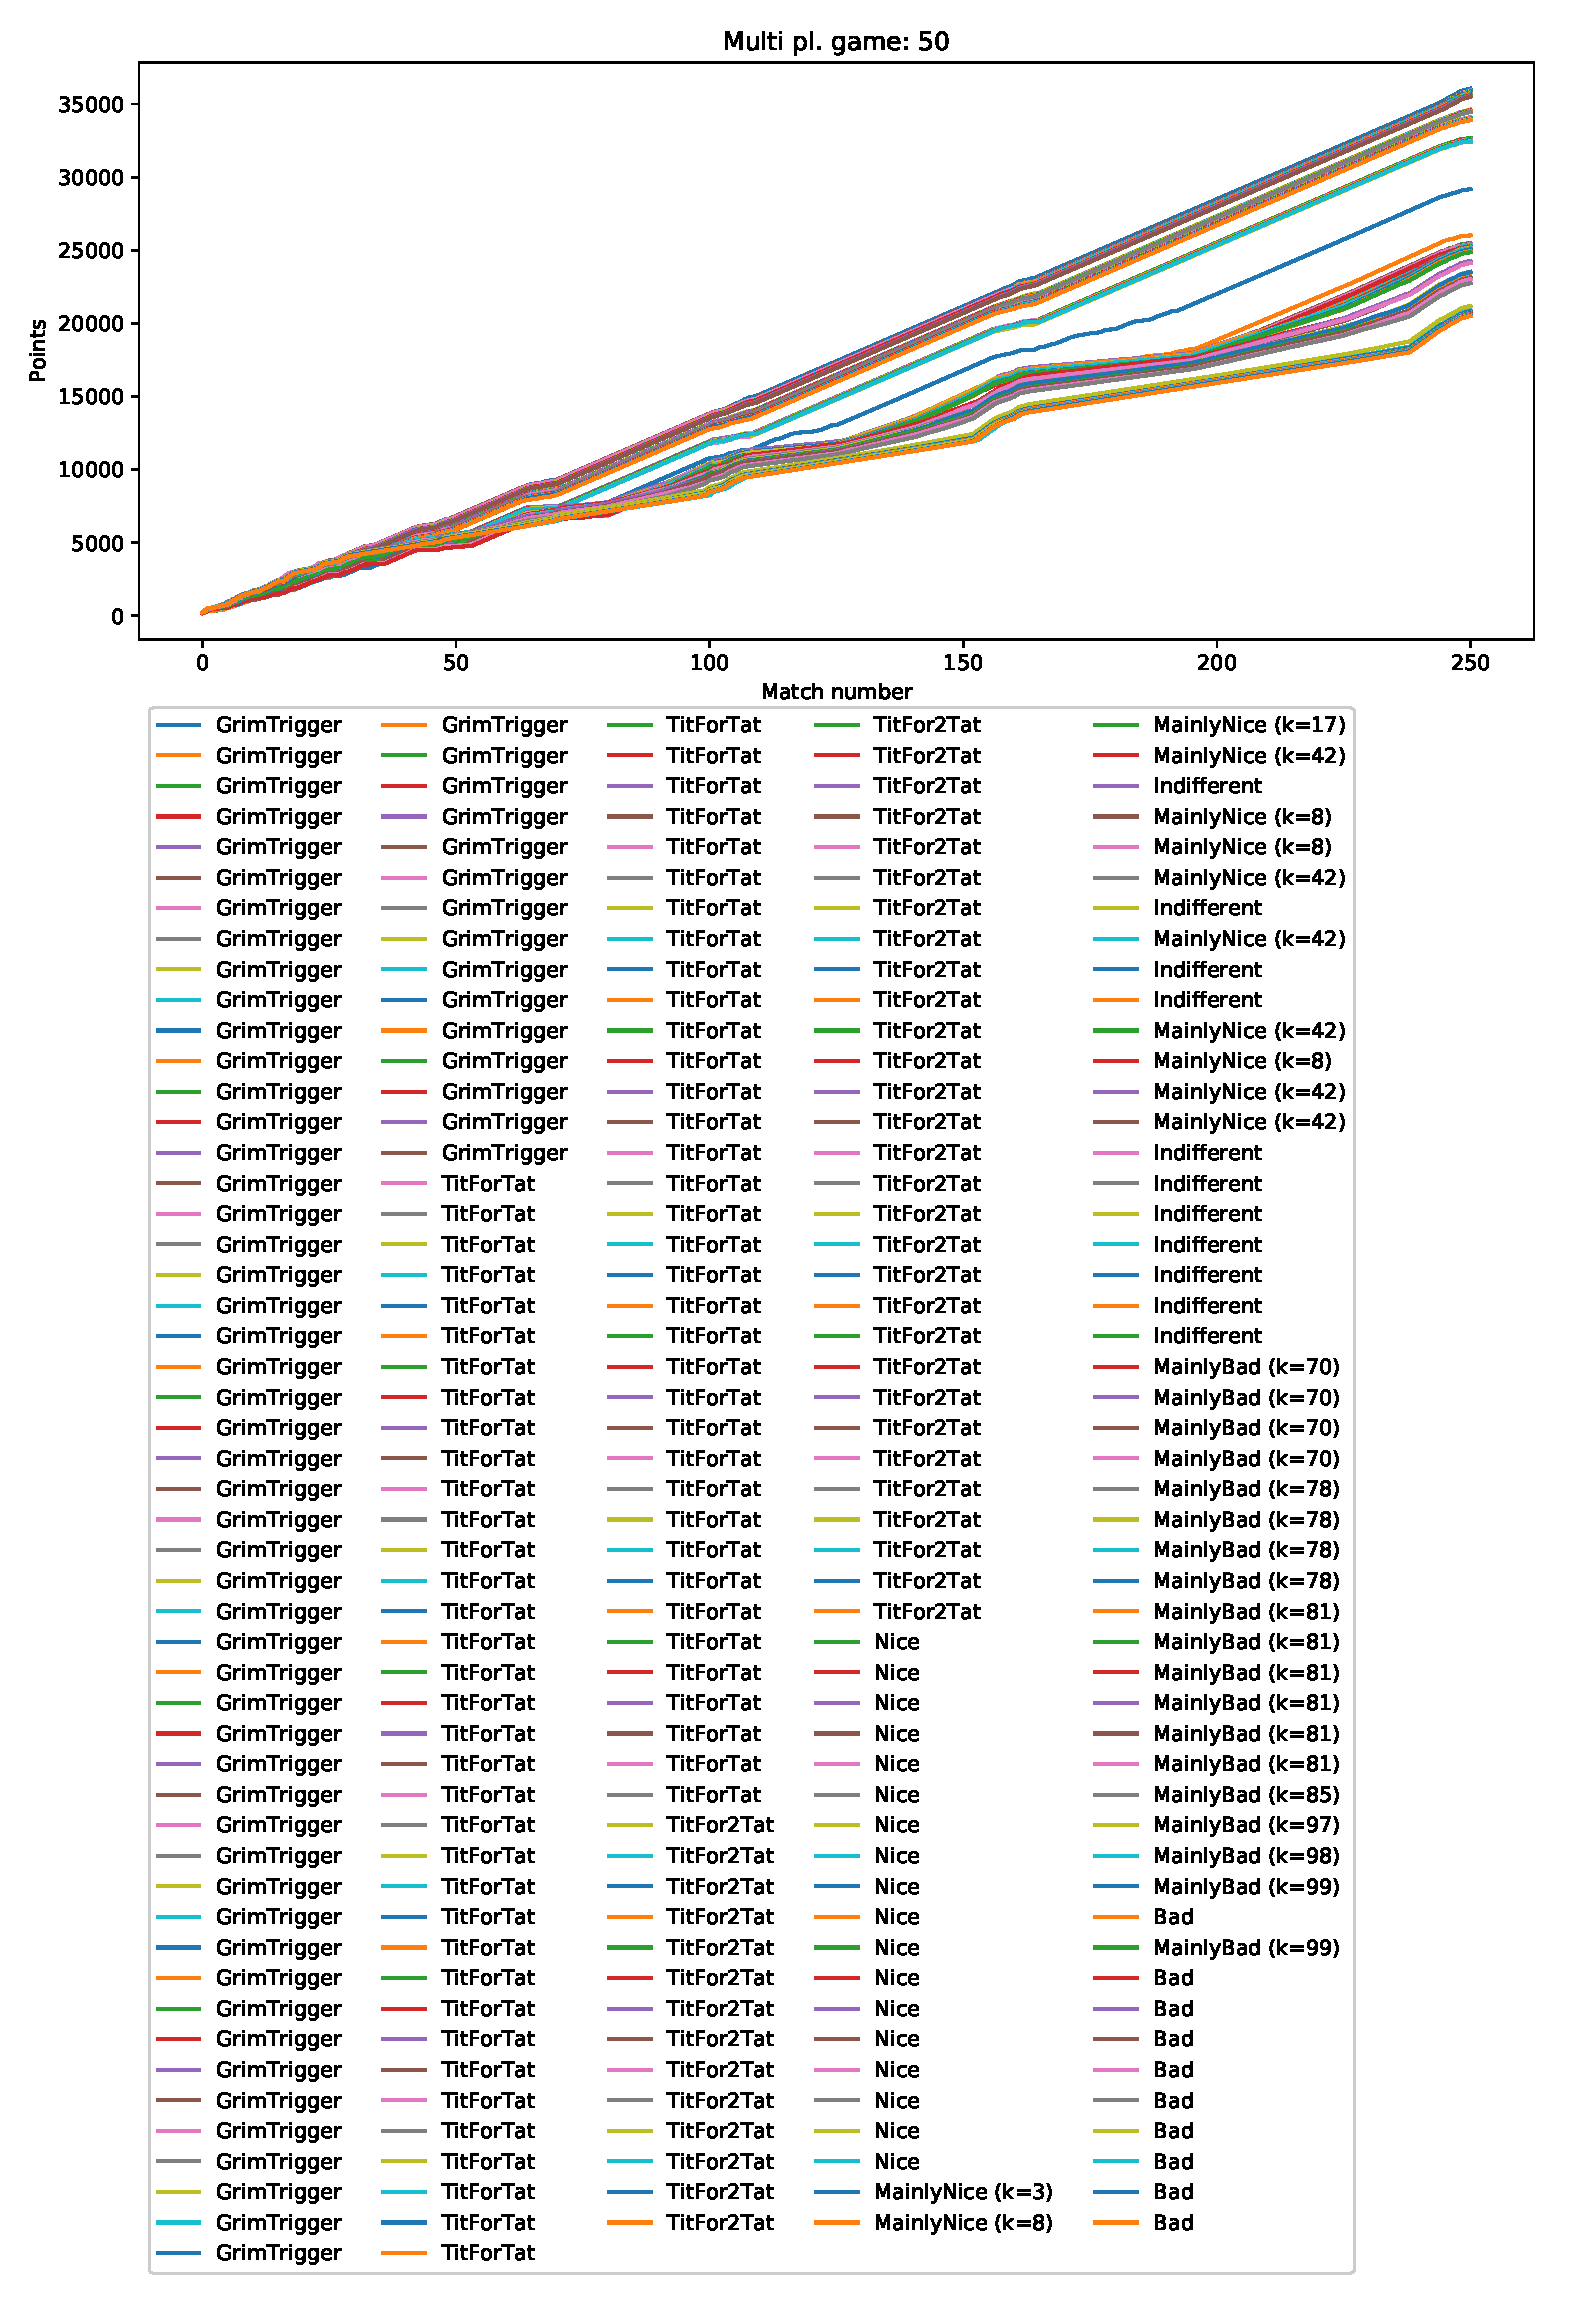
\includegraphics[width=1\columnwidth]{../img/ripdmp-incr/alt1/ripdmp-scores-increasing-pop-50-r4}
    \caption{Last iteration scores ($it=4$)}
    \label{fig:incrLI}
\end{figure}

It is interesting to note how Wu and Axelrod \cite{IPDnoise} exploit this behavior to react to noise in the game: by slightly altering the \textit{TfT} strategy in both directions, adding generosity (some percentage of opponent's defections go unpunished) or contrition (avoid responding to a defect move when a player's previous defection was unintended), the ``error'' can be quickly recovered and cooperation can be successfully restored. Note, however, that in this work these two variations of the \textit{TfT} strategy are not implemented.

The other alternatives give similar results that do not change our considerations. Full details can be found in the \hyperref[s:appendix]{Appendix} (Tables~[\ref{tab:ripdmp-incrA2},\ref{tab:ripdmp-incrA3}] and Figures~[\ref{fig:incrRa2},\ref{fig:incrRa3}]). The only partial exception to this trend is alternative 3 because the score obtained by each player is not equally distributed as in the other two cases. This benefits the strategies that have achieved the best overall score and disadvantages all the other strategies.

\section{rMPIPD with changing strategies} \label{s:crIPDMP}
A step further is made by allowing players to change their strategies in the rIPDMP setup, from which the main structure is unaltered.
Each player has a gene $c$, representing his attitude to cooperate. This value is initially assigned a value of $c=k/100$, where $k$ is the probability of cooperating for random, \textit{Bad} and \textit{Nice} strategies. For \textit{GrT}, \textit{TfT} and \textit{Tf2T} $c$ is set to $0.5$ since these strategies do not have an intrinsic specific attitude for cooperating.
 
A single round of the game goes as follow: a rIPDMP's round is played, then new players are generated following the first alternative presented in the previous \autoref{ss:rIPDMPi}, and for each one of the ``old'' players a new $c$ is generated and their strategies changes accordingly. This will be repeated until convergence or a maximum number of iterations is reached.

Two alternatives are proposed to change $c$ after each round.
\begin{enumerate}
    \item For each player, a new random $c_N$ is generated
    \item The change of strategy is again based on players' ranking and probability. Bad players (those with $k>50$) have their $c$ updated as
    $c_N = (c+(i/num\_players)^2)/2$, that is, players high in the chart will go to a \textit{less} cooperative behavior and vice-versa.
    Good players are updated according to $c_N = (c+((1-i)/num\_players)^2)/2$, that is, opposite from before, players high in the chart will have a \textit{more} cooperative behavior and vice-versa.
\end{enumerate}

At this point, if the absolute value of the difference between the old $c$ and the new $c_N$ is greater than a threshold (set to $0.1$) the strategy will change. 
The new strategy is picked from a set made of $6$ different random strategies plus \textit{GrT, TfT, Tf2T}.
Note that \textit{GrT} is not available if the player's strategy is going to change towards the good side: in our vision, \textit{GrT} is a revengeful strategy, and the fact that others call it \textit{spiteful} also support that. We cannot propose this strategy if someone wants to be a ``good'' player.
The random strategy generation is bounded based on the strategy's $id$ ($k$ for probability strategies) and $c_N$.\footnote{As a consequence, 4 different cases have to be handled, depending on $id$ or $50$ being considered inside the $\min$ and $\max$ functions in the bounds.}
\begin{itemize}
    \item if $c_N \ge 0.5$ the strategies stay on the ``good'' side, between $(1-c)\times 100$ and $\min(id,50)$.
    \item if $c_N < 0.5$ the strategies stay on the ``bad'' side, between $\max(id,50)$ and $(1-c)\times 100$.
\end{itemize}
\textit{GrT} is forced to evolve only towards less cooperative behavior since it is a revengeful strategy, and \textit{TfT, Tf2T} are treated as being in the middle of the range, like \textit{Indifferent}, since they are reactive ones.

Details on the evolution of the population can be found in \autoref{tab:cripdmp}.
The other alternative is presented on \autoref{tab:cripdmpA2} and \autoref{fig:incrC2}.

\textbf{Todo maybe expand?}
In both cases it is easy to see that the same strategies of the other study cases takes the lead, namely \textit{GrT}, \textit{Tf(2)T} and \textit{Bad} players. In our simulations we have found that either with a random bias toward cooperation or with a deterministic one the evolution of the population still converges toward the strategies we have identified as winningly.

The metrics ``To more(less) cooperative'' are purely indicative to count where the inclinance of the players moves. One can go to a less cooperative behaviour but still became a \textit{GrT}.

Finally, the total number of players with random strategy are more or less the same, without substancial differences betweeen the two populations.

\begin{figure}[!ht]
    \centering
    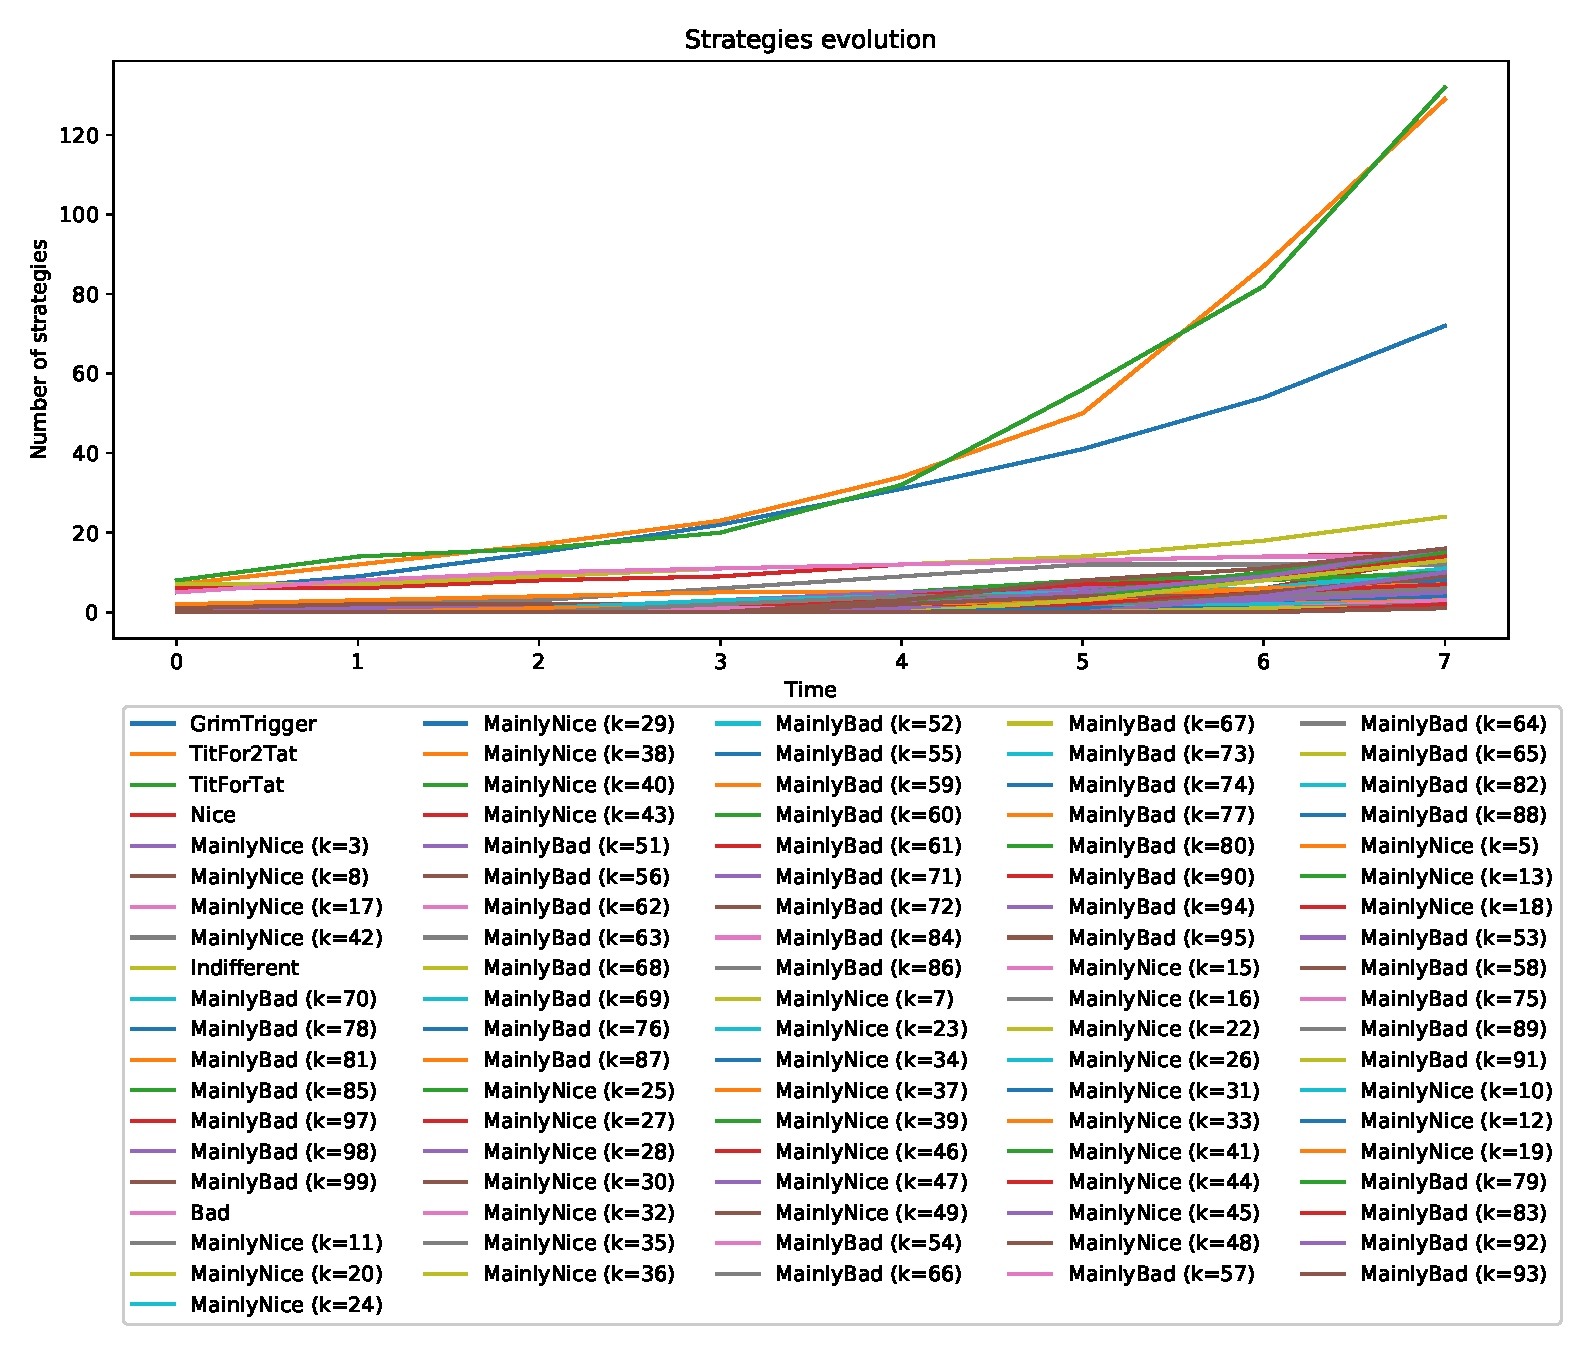
\includegraphics[width=1\columnwidth]{../img/cipdmp-incr/alt1/cipdmp-evolution-increasing-pop-50}
    \caption{Evolution of rIPDMP, changing strategies, increasing pop. from 50}
    \label{fig:incrC}
\end{figure}

\begin{figure}[!ht]
    \centering
    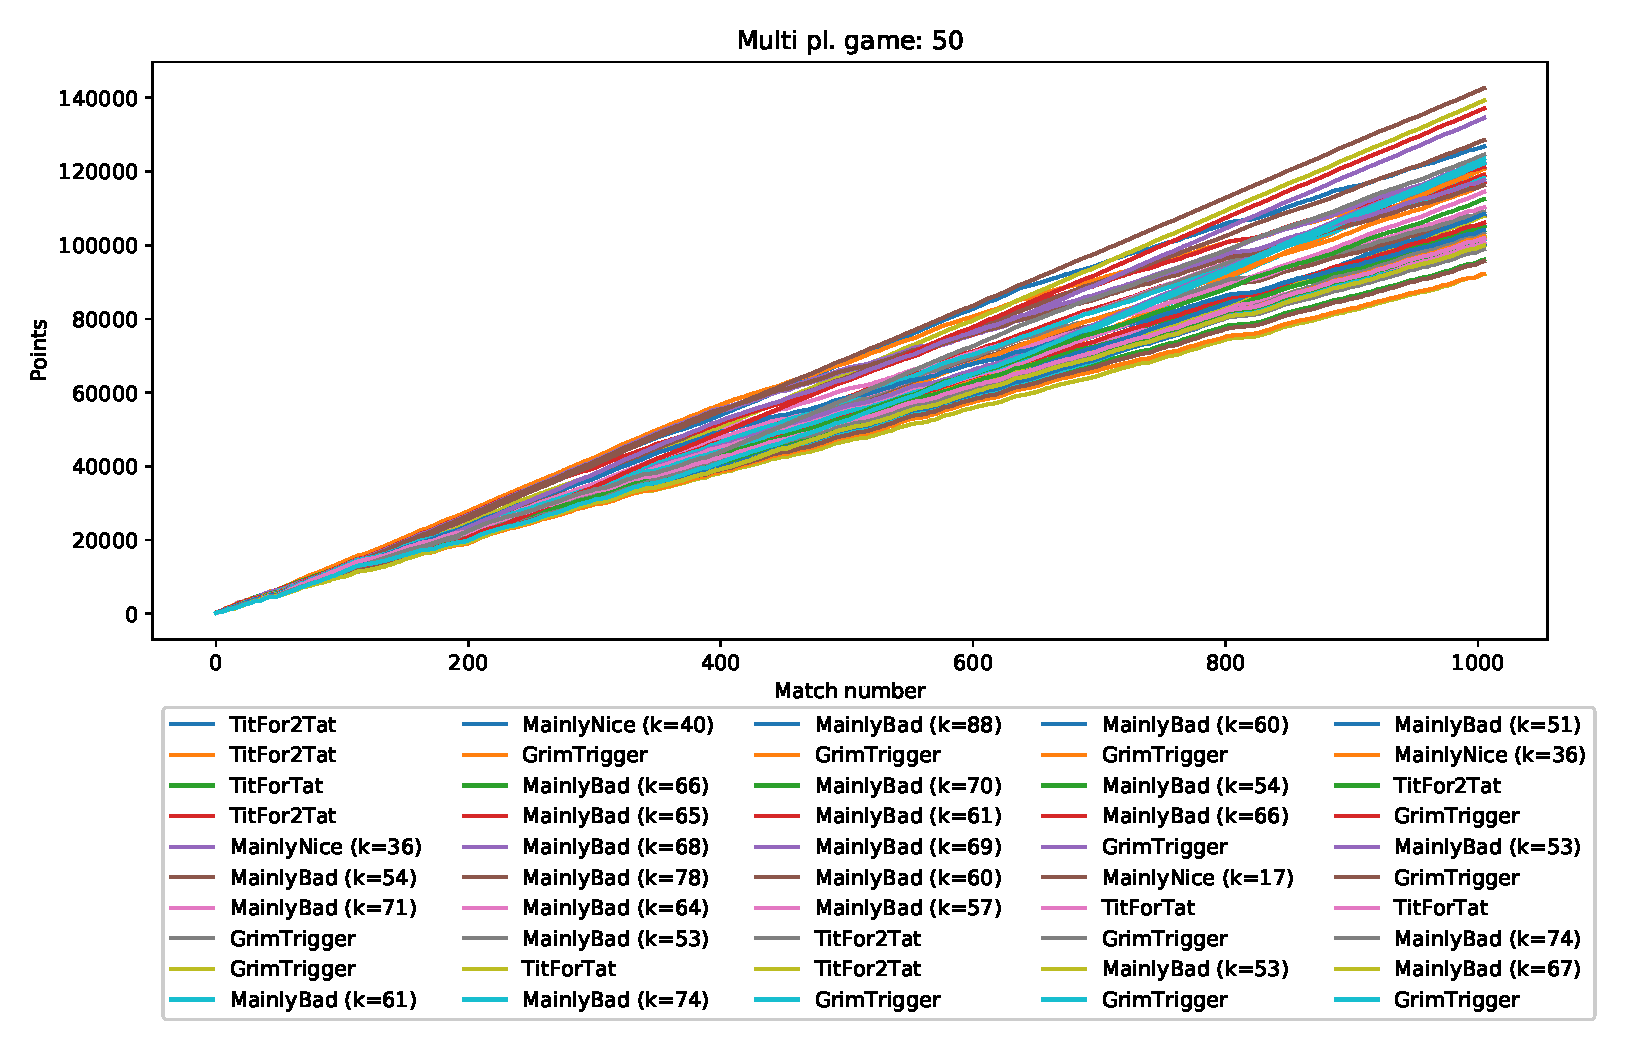
\includegraphics[width=1\columnwidth]{../img/cipdmp-incr/alt1/cipdmp-scores-increasing-pop-50-r0}
    \caption{First iteration scores ($it=0$)}
    \label{fig:incrCFI}
\end{figure}

\begin{figure}[!ht]
    \centering
    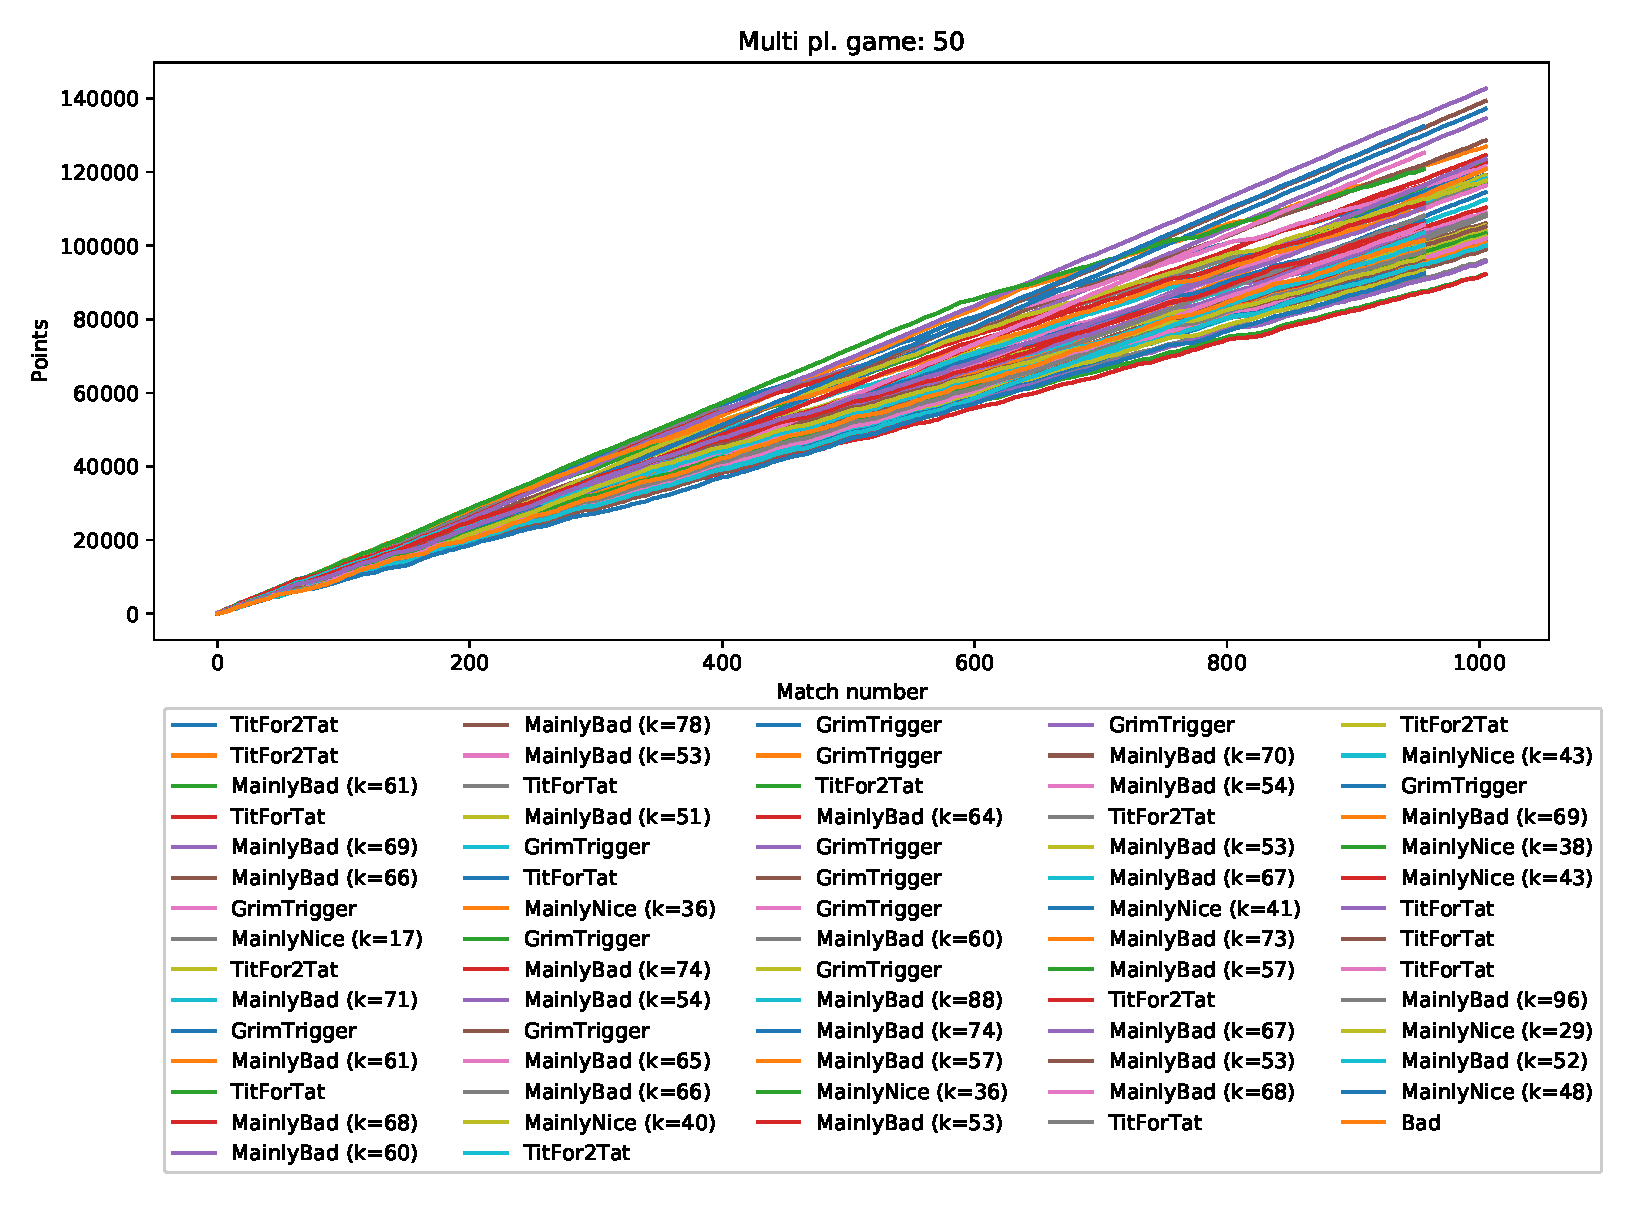
\includegraphics[width=1\columnwidth]{../img/cipdmp-incr/alt1/cipdmp-scores-increasing-pop-50-r2}
    \caption{Middle iteration scores ($it=2$)}
    \label{fig:incrCMI}
\end{figure}

\begin{figure}[!ht]
    \centering
    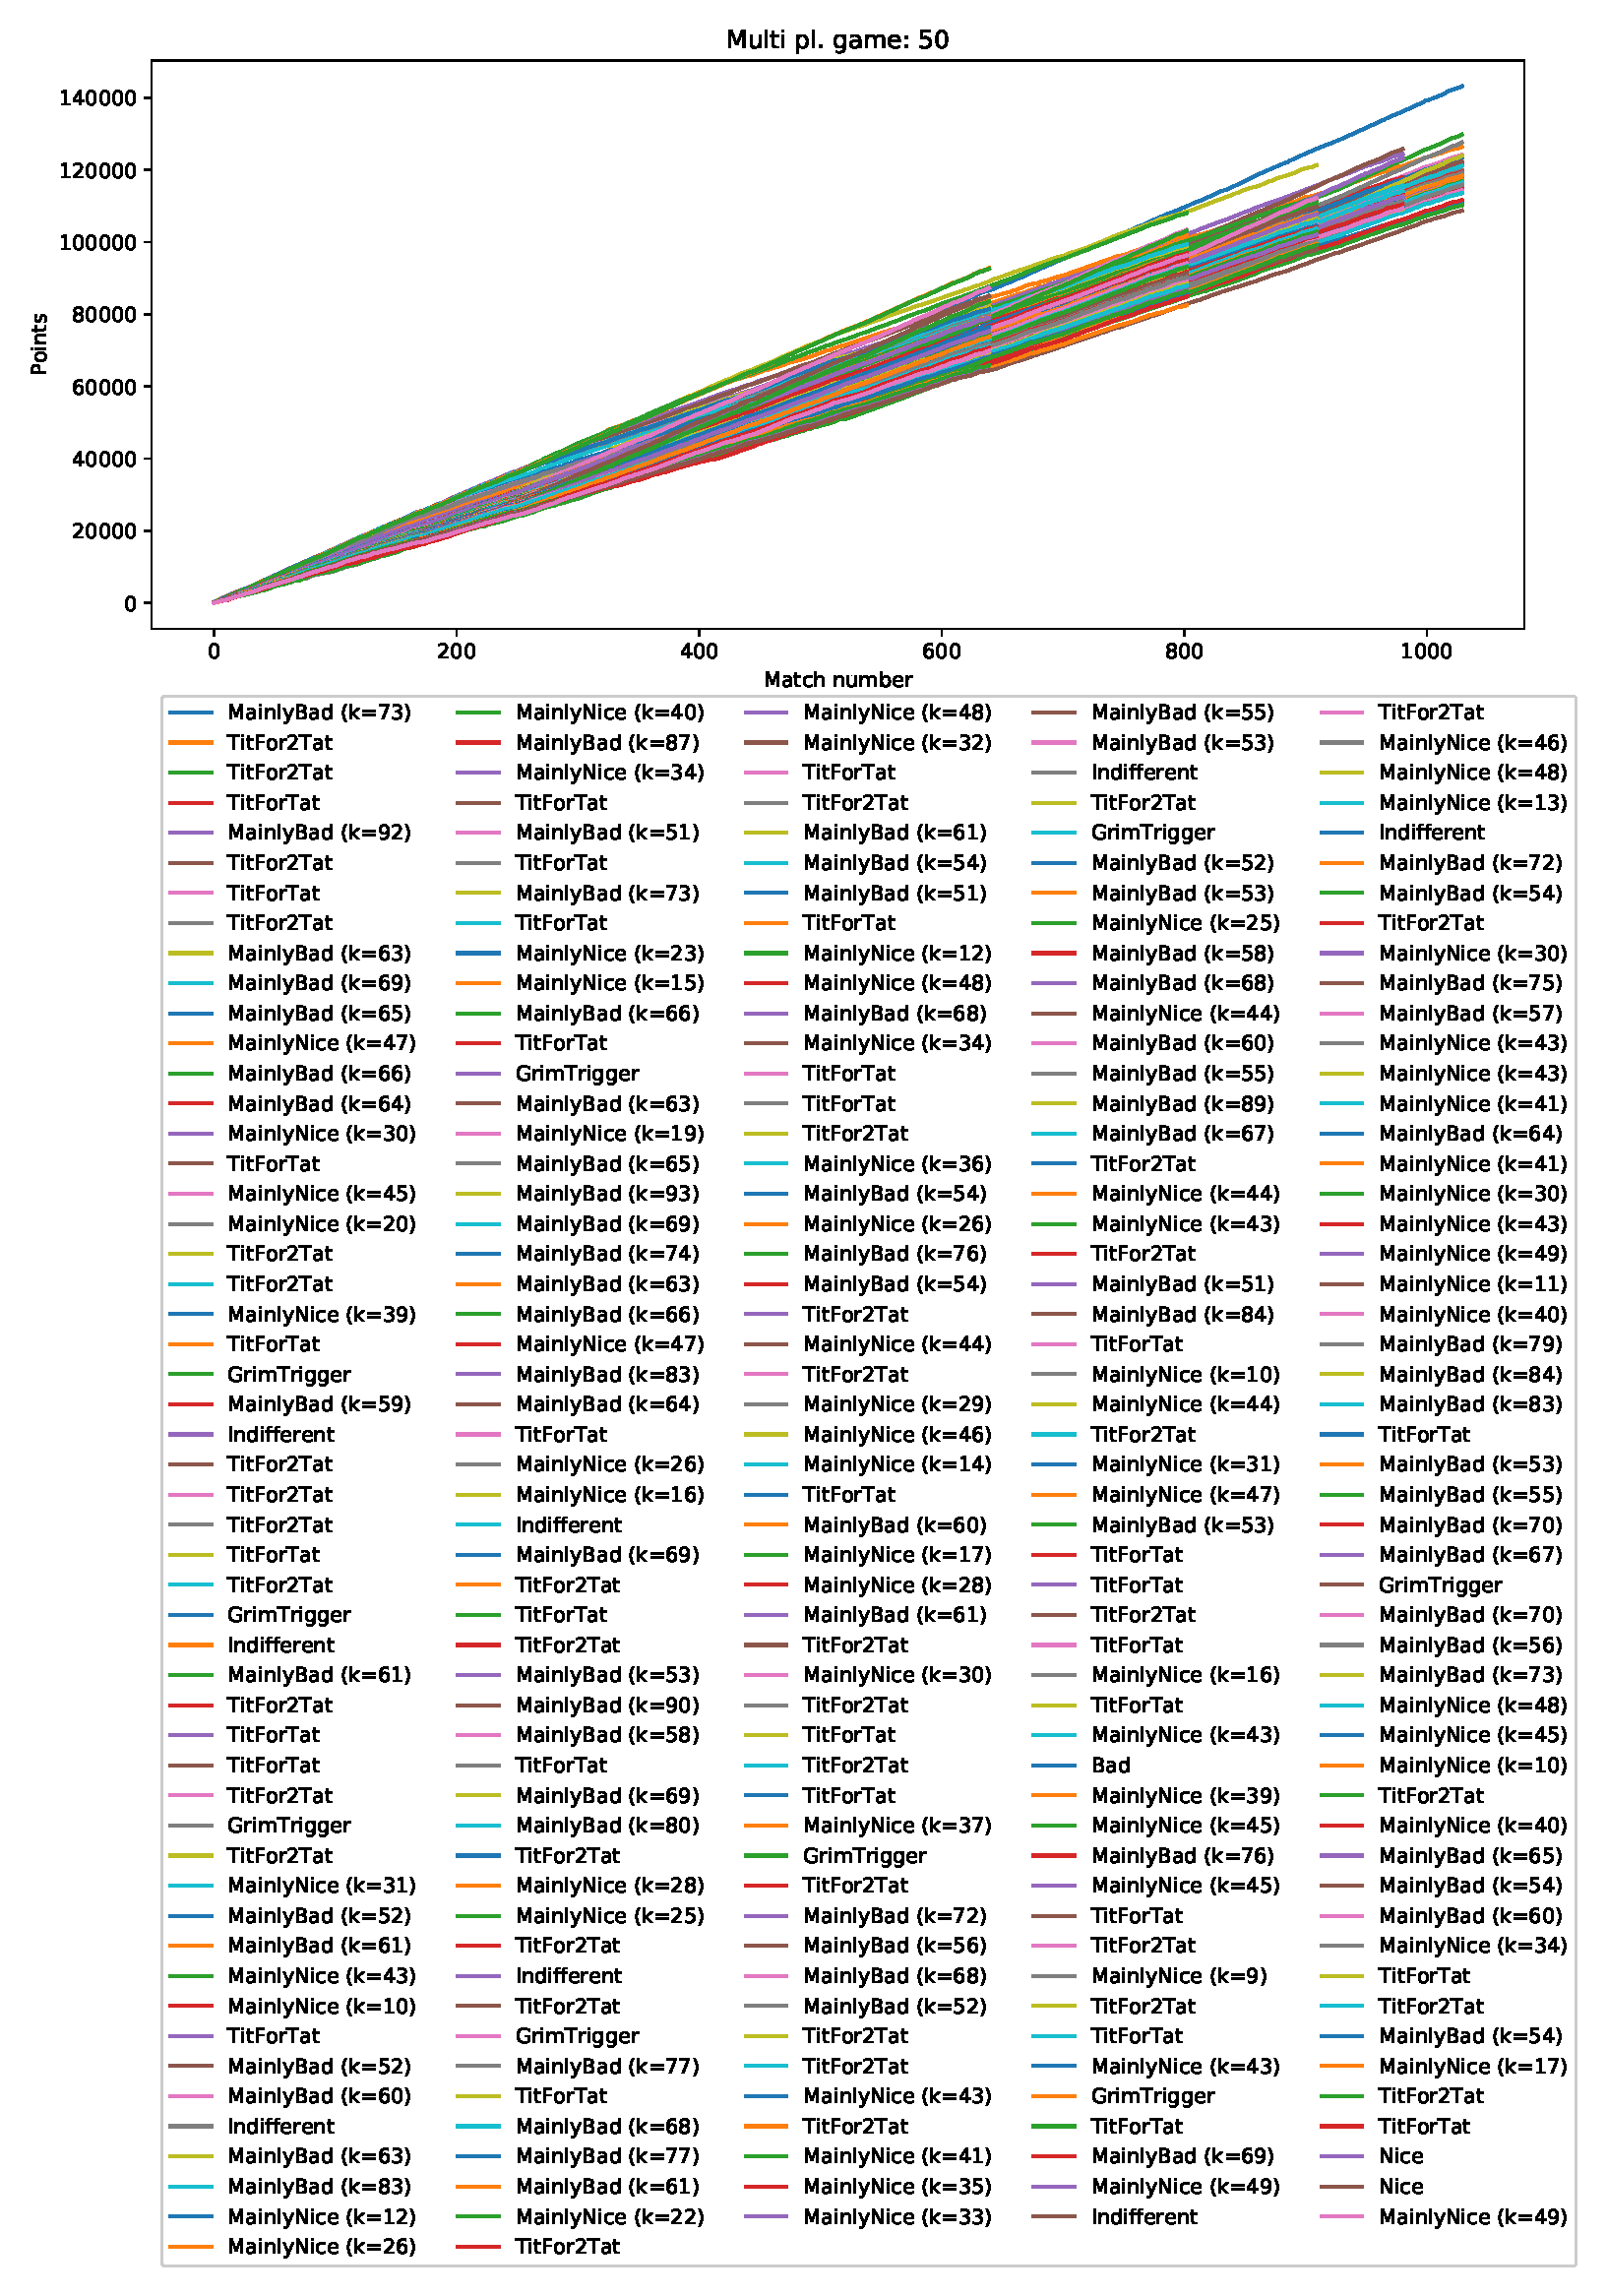
\includegraphics[width=1\columnwidth]{../img/cipdmp-incr/alt1/cipdmp-scores-increasing-pop-50-r4}
    \caption{Last iteration scores ($it=4$)}
    \label{fig:incrCLI}
\end{figure}

\section{Machine Learning approaches} \label{s:ml}
Since the beginning of research on this subject, studies have been developed to find some pattern that can be exploited by learning algorithms.
By the formulation of the IPD game, if such a pattern exists, it has to be learned using unsupervised techniques, since the final outcome of the players depends on their actions.

Players should learn to cooperate --- equivalently, to enhance their altruism --- and here the aim is to do so by adaptively \textit{learning} a strategy. A hindrance is that, in the PD, the Nash Equilibrium solution (as stated before, to defect) is not a desirable learning target.~\cite{coopSeqRL}

Reinforcement learning (RL) is an unsupervised learning technique whereby the system must select an output (in case of PD, an action: cooperate or defect) for which it receives a scalar evaluation. RL requires to find the best output for any given input, and is based on the idea that the tendency to produce an action should be strengthened if the action led to favorable results, and weakened otherwise.~\cite{sandholmRL}

Sandholm and Crites \cite{sandholmRL} employed recurrent neural networks (RNN) and the Q-learning algorithm, a particular RL procedure that works by estimating the value of state-action pairs, to train agents to play against the \textit{TfT} strategy and against an unknown opponent. While the first task was easily learned, the second one proved to be more difficult due to non-stationary behavior and lack of \textit{a priori} knowledge of a policy to encourage cooperation.
More recently, Wang \cite{kedaoRL} extended this study with newly developed structures for the RNN part, to test both finite and infinite iterations setups. However, his tests led to pretty much the same results Sandholm had previously obtained.
Finally, evolutionary and particle swarm algorithms are used by Harper \textit{et al.} in a very extensive study \cite{plosRLdominant} to train strategies to perform well against over 170 distinct opponents even in noisy tournaments.

What is noted from the literature is that it is an easy task for a player to learn to compete against a deterministic player, while it is indeed difficult to generalize to an opponent with unspecified behavior.

This is a very specific problem that, given the restrictions of the game, cannot be fully solved by machine learning procedures. As a matter of fact, the rules of the game restrict it in a very simple but powerful area where this kind of methods gain their strengths: information. In particular, we cannot allow the algorithm to know the opponent moves in advance, or their type, or how much the game will go on or any other information that would be viable and helpful to solve the game. Furthermore, the intrinsic ``incoherence'' between rational behavior and optimal outcome (the Nash Equilibrium vs Pareto efficiency choices) makes the task extremely difficult to be fully examined by machine learning approaches.

\section{Conclusions and future work} \label{s:conc}
We presented our implementation of the Prisoner's Dilemma and we analyzed the outcomes of all the study-cases.
We pointed out that there is no ``best'' strategy for the game: each individual strategy will work better when matched against a ``worse'' strategy. When paired with a mindless strategy like probability strategies, \textit{TfT} sinks to its opponent's level. This is why \textit{TfT} is not the ``best'' strategy. In order to win, a player should figure out its opponent's strategy and then pick a strategy that is best suited for the situation.
We also showed advances in the literature that try to address the iterative version of the game with machine learning approaches, noting that it is no trivial task. 
An important insight is also the tight dependance with respect to the initial population and seed: this factor could vary the results in an unpredictable and unexpected way. It is not trivial to address which player would be the winner given an initial population.
Finally the introduction of the possibility to change the strategies within the tournament does not take variance in the final results but only in the way the population gets there.

This work can be easily extended in many ways and have future development: i.e. a lot of new and more complex strategies were created since the original tournaments made by Axelrod and these may be incorporated in the analysis, alongside the already available ones.
The Axelrod library, \cite{Knight2016Axel,axel-lib} written in Python and also used by \cite{plosRLdominant}, contains more than 270 standard, deterministic and learning-based strategies, and is now the reference framework to study the prisoner's dilemma.
Furthermore, research may be directed to find and implement different features or network structures that achieve better results with automated learning. It would be also interesting to extend the memory of the players to the whole history of the game, allowing them to make predictions and belief on the type of the opponents.

\balance
\bibliographystyle{IEEEtran}
\bibliography{report}

\onecolumn
\appendix[Additional figures and tables of tournament results] \label{s:appendix}

%\appendices
%\section{Additional figures} \label{a:fig}
%\section{Tables of tournament results} \label{a:tab} 

\begin{table}[ht]
    \caption{2-players IPD, statistics}
    \label{tab:ipd2p}
    \centering
    \begin{tabular}{ll|rrrr|rrrr} \toprule
           \multicolumn{2}{c}{Strategies}     & \multicolumn{4}{c}{Scores Player 1} & \multicolumn{4}{c}{Scores Player 2} \\
        Player 1          & Player 2          &   avg &   std &  yield &    achieve &   avg &   std &  yield &    achieve \\ \midrule
        Bad               & Bad               &  50.0 &  0.00 & 100.00 &      20.00 &  50.0 &  0.00 & 100.00 &      20.00 \\
        Bad               & TitFor2Tat        &  58.0 &  0.00 & 100.00 &      23.20 &  48.0 &  0.00 &  96.00 &      19.51 \\
        Bad               & GrimTrigger       &  54.0 &  0.00 & 100.00 &      21.60 &  49.0 &  0.00 &  98.00 &      19.76 \\
        Bad               & Indifferent       & 146.0 & 11.03 & 100.00 &      58.40 &  26.0 &  2.76 &  52.00 &      12.84 \\
        Bad               & MainlyNice (k=27) & 205.6 & 11.66 & 100.00 &      82.24 &  11.1 &  2.91 &  22.20 &       6.39 \\
        Bad               & TitForTat         &  54.0 &  0.00 & 100.00 &      21.60 &  49.0 &  0.00 &  98.00 &      19.76 \\
        Bad               & MainlyBad (k=72)  & 102.0 & 15.39 & 100.00 &      40.80 &  37.0 &  3.85 &  74.00 &      16.48 \\
        Bad               & Nice              & 250.0 &  0.00 & 100.00 &     100.00 &   0.0 &  0.00 &   0.00 &       0.00 \\
        TitFor2Tat        & TitFor2Tat        & 150.0 &  0.00 &  60.00 &     100.00 & 150.0 &  0.00 &  60.00 &     100.00 \\
        TitFor2Tat        & GrimTrigger       & 150.0 &  0.00 &  60.00 &     100.00 & 150.0 &  0.00 &  60.00 &     100.00 \\
        TitFor2Tat        & Indifferent       &  91.4 &  4.52 &  62.50 &      52.76 & 160.4 & 11.19 &  79.57 &      79.78 \\
        TitFor2Tat        & MainlyNice (k=27) & 110.3 &  8.54 &  59.34 &      68.97 & 164.3 &  5.80 &  71.78 &      90.45 \\
        TitFor2Tat        & TitForTat         & 150.0 &  0.00 &  60.00 &     100.00 & 150.0 &  0.00 &  60.00 &     100.00 \\
        TitFor2Tat        & MainlyBad (k=72)  &  73.1 &  4.18 &  71.23 &      36.40 & 127.1 & 14.69 &  87.02 &      57.08 \\
        TitFor2Tat        & Nice              & 150.0 &  0.00 &  60.00 &     100.00 & 150.0 &  0.00 &  60.00 &     100.00 \\
        GrimTrigger       & GrimTrigger       & 150.0 &  0.00 &  60.00 &     100.00 & 150.0 &  0.00 &  60.00 &     100.00 \\
        GrimTrigger       & Indifferent       & 149.2 & 11.50 &  98.43 &      60.51 &  30.7 &  4.12 &  53.99 &      15.39 \\
        GrimTrigger       & MainlyNice (k=27) & 194.8 & 11.15 &  97.57 &      79.75 &  22.3 &  8.22 &  35.21 &      12.68 \\
        GrimTrigger       & TitForTat         & 150.0 &  0.00 &  60.00 &     100.00 & 150.0 &  0.00 &  60.00 &     100.00 \\
        GrimTrigger       & MainlyBad (k=72)  & 101.4 & 12.19 &  98.23 &      41.02 &  41.9 &  3.39 &  75.36 &      18.73 \\
        GrimTrigger       & Nice              & 150.0 &  0.00 &  60.00 &     100.00 & 150.0 &  0.00 &  60.00 &     100.00 \\
        Indifferent       & Indifferent       & 112.3 & 10.21 &  74.56 &      56.17 & 112.3 & 10.21 &  74.56 &      56.17 \\
        Indifferent       & MainlyNice (k=27) & 150.3 & 16.27 &  77.36 &      75.42 &  97.3 & 12.86 &  64.02 &      54.59 \\
        Indifferent       & TitForTat         & 117.5 &  7.27 &  73.92 &      60.08 & 115.5 &  7.99 &  73.39 &      59.30 \\
        Indifferent       & MainlyBad (k=72)  &  77.5 & 14.15 &  70.26 &      38.68 & 126.5 & 11.59 &  84.81 &      57.50 \\
        Indifferent       & Nice              & 200.8 &  5.00 &  80.32 &     100.00 &  73.8 &  7.49 &  49.62 &      49.20 \\
        MainlyNice (k=27) & MainlyNice (k=27) & 132.7 & 12.88 &  67.31 &      75.06 & 132.7 & 12.88 &  67.31 &      75.06 \\
        MainlyNice (k=27) & TitForTat         & 135.6 &  3.83 &  67.33 &      77.61 & 133.6 &  4.80 &  66.86 &      76.82 \\
        MainlyNice (k=27) & MainlyBad (k=72)  &  61.9 &  8.84 &  56.42 &      34.92 & 170.4 & 10.44 &  86.87 &      77.27 \\
        MainlyNice (k=27) & Nice              & 179.8 &  4.33 &  71.92 &     100.00 & 105.3 &  6.50 &  55.26 &      70.20 \\
        TitForTat         & TitForTat         & 150.0 &  0.00 &  60.00 &     100.00 & 150.0 &  0.00 &  60.00 &     100.00 \\
        TitForTat         & MainlyBad (k=72)  &  87.6 &  7.05 &  81.94 &      40.00 &  92.1 &  7.03 &  83.34 &      41.70 \\
        TitForTat         & Nice              & 150.0 &  0.00 &  60.00 &     100.00 & 150.0 &  0.00 &  60.00 &     100.00 \\
        MainlyBad (k=72)  & MainlyBad (k=72)  &  88.5 & 12.09 &  81.42 &      40.03 &  88.5 & 12.09 &  81.42 &      40.03 \\
        MainlyBad (k=72)  & Nice              & 222.0 &  8.20 &  88.80 &     100.00 &  42.0 & 12.30 &  38.68 &      28.00 \\
        Nice              & Nice              & 150.0 &  0.00 &  60.00 &     100.00 & 150.0 &  0.00 &  60.00 &     100.00 \\ \bottomrule
    \end{tabular}
\end{table}

\begin{table}[ht]
    \caption{2-players IPD, overall yield and achieve}
    \label{tab:ipd2pavg}
    \centering
    \begin{tabular}{l|rr} \toprule
        Strategy          &  yield & achieve \\ \midrule
        Bad               & 100.00 &   43.09 \\
        GrimTrigger       &  76.91 &   77.89 \\
        Indifferent       &  70.73 &   54.95 \\
        MainlyBad (k=72)  &  82.56 &   49.87 \\
        MainlyNice (k=27) &  58.17 &   58.53 \\
        Nice              &  49.29 &   71.93 \\
        TitFor2Tat        &  65.45 &   75.29 \\
        TitForTat         &  68.91 &   77.32 \\ \bottomrule
    \end{tabular}
\end{table}

\begin{table}[ht]
    \caption{50-players IPD, sorted by points, statistics}
    \label{tab:ipdmp50}
    \centering
    \begin{tabular}{l|rrrr|rrrrr} \toprule
                          &     \multicolumn{4}{c}{Points}     & \multicolumn{2}{c}{Coop. count} & \multicolumn{2}{c}{Defect count} &          \\
        Strategy          &    avg &    std &  yield & achieve &    avg &                    std &    avg &                     std & Coop. \% \\ \midrule
        GrimTrigger       & 6406.5 &  80.89 &  77.66 &   73.21 & 1334.5 &                  18.42 & 1115.5 &                   18.42 &    54.47 \\
        GrimTrigger       & 6393.8 &  56.80 &  77.91 &   73.90 & 1317.6 &                  21.68 & 1132.4 &                   21.68 &    53.78 \\
        GrimTrigger       & 6385.3 &  72.00 &  77.06 &   73.85 & 1336.4 &                  23.56 & 1113.6 &                   23.56 &    54.55 \\
        GrimTrigger       & 6382.0 &  88.09 &  77.76 &   73.59 & 1327.7 &                  23.79 & 1122.3 &                   23.79 &    54.19 \\
        GrimTrigger       & 6380.4 &  92.53 &  78.39 &   73.35 & 1343.3 &                  37.35 & 1106.7 &                   37.35 &    54.83 \\
        TitForTat         & 5884.6 &  26.69 &  71.37 &   72.60 & 1664.8 &                  10.76 &  785.2 &                   10.76 &    67.95 \\
        TitForTat         & 5882.7 &  27.79 &  71.41 &   72.55 & 1662.7 &                  14.49 &  787.3 &                   14.49 &    67.87 \\
        TitForTat         & 5881.4 &  26.80 &  70.99 &   73.34 & 1665.1 &                  11.69 &  784.9 &                   11.69 &    67.96 \\
        TitForTat         & 5880.2 &  34.27 &  71.13 &   72.82 & 1662.7 &                  14.85 &  787.3 &                   14.85 &    67.87 \\
        TitForTat         & 5878.9 &  32.66 &  71.47 &   72.29 & 1660.8 &                  13.31 &  789.2 &                   13.31 &    67.79 \\
        TitForTat         & 5875.6 &  32.89 &  71.10 &   72.58 & 1661.3 &                  13.60 &  788.7 &                   13.60 &    67.81 \\
        TitForTat         & 5862.2 &  22.34 &  71.23 &   72.51 & 1654.7 &                   9.78 &  795.3 &                    9.78 &    67.54 \\
        TitForTat         & 5861.2 &  27.54 &  71.27 &   72.66 & 1655.7 &                  10.52 &  794.3 &                   10.52 &    67.58 \\
        TitFor2Tat        & 5648.6 &  16.61 &  67.62 &   72.29 & 1829.7 &                  10.07 &  620.3 &                   10.07 &    74.68 \\
        TitFor2Tat        & 5644.3 &  18.15 &  67.25 &   71.73 & 1834.4 &                  11.92 &  615.6 &                   11.92 &    74.87 \\
        TitFor2Tat        & 5639.4 &  18.24 &  67.14 &   72.01 & 1833.6 &                  18.54 &  616.4 &                   18.54 &    74.84 \\
        TitFor2Tat        & 5637.9 &  22.20 &  67.10 &   72.51 & 1821.5 &                  14.67 &  628.5 &                   14.67 &    74.35 \\
        TitFor2Tat        & 5636.4 &  34.72 &  67.09 &   72.63 & 1824.9 &                  19.76 &  625.1 &                   19.76 &    74.49 \\
        TitFor2Tat        & 5636.4 &  18.00 &  67.33 &   71.98 & 1825.7 &                   8.56 &  624.3 &                    8.56 &    74.52 \\
        TitFor2Tat        & 5621.5 &  29.34 &  67.45 &   71.36 & 1817.2 &                  17.42 &  632.8 &                   17.42 &    74.17 \\
        MainlyBad (k=78)  & 5456.8 &  40.52 &  85.00 &   49.18 &  545.4 &                  22.11 & 1904.6 &                   22.11 &    22.26 \\
        MainlyBad (k=85)  & 5424.8 &  59.18 &  89.74 &   47.57 &  373.9 &                  17.92 & 2076.1 &                   17.92 &    15.26 \\
        MainlyBad (k=81)  & 5416.4 &  60.69 &  87.56 &   47.69 &  469.9 &                  15.43 & 1980.1 &                   15.43 &    19.18 \\
        MainlyBad (k=81)  & 5411.3 &  65.52 &  87.63 &   48.21 &  459.6 &                  19.84 & 1990.4 &                   19.84 &    18.76 \\
        MainlyBad (k=70)  & 5396.5 &  63.52 &  80.99 &   50.32 &  728.7 &                  17.36 & 1721.3 &                   17.36 &    29.74 \\
        MainlyBad (k=97)  & 5387.7 &  64.01 &  97.66 &   45.52 &   74.5 &                   6.52 & 2375.5 &                    6.52 &     3.04 \\
        MainlyBad (k=99)  & 5379.8 &  62.25 &  99.21 &   43.99 &   26.3 &                   5.77 & 2423.7 &                    5.77 &     1.07 \\
        Bad               & 5362.4 &  78.10 & 100.00 &   44.00 &    0.0 &                   0.00 & 2450.0 &                    0.00 &     0.00 \\
        Bad               & 5359.2 &  41.10 & 100.00 &   44.33 &    0.0 &                   0.00 & 2450.0 &                    0.00 &     0.00 \\
        MainlyBad (k=98)  & 5352.7 &  35.40 &  98.74 &   43.58 &   48.7 &                   5.46 & 2401.3 &                    5.46 &     1.99 \\
        Bad               & 5343.2 &  41.91 & 100.00 &   43.87 &    0.0 &                   0.00 & 2450.0 &                    0.00 &     0.00 \\
        Bad               & 5330.8 &  33.93 & 100.00 &   43.51 &    0.0 &                   0.00 & 2450.0 &                    0.00 &     0.00 \\
        Bad               & 5322.0 &  21.00 & 100.00 &   43.61 &    0.0 &                   0.00 & 2450.0 &                    0.00 &     0.00 \\
        Indifferent       & 5275.9 &  89.52 &  69.73 &   53.26 & 1218.6 &                  28.88 & 1231.4 &                   28.88 &    49.74 \\
        Indifferent       & 5265.9 &  89.16 &  69.80 &   53.75 & 1219.9 &                  21.74 & 1230.1 &                   21.74 &    49.79 \\
        Indifferent       & 5265.5 &  67.17 &  69.57 &   53.43 & 1221.6 &                  15.01 & 1228.4 &                   15.01 &    49.86 \\
        Indifferent       & 5248.7 &  56.13 &  69.04 &   53.87 & 1222.9 &                  21.45 & 1227.1 &                   21.45 &    49.91 \\
        Indifferent       & 5240.5 &  62.17 &  69.48 &   52.91 & 1217.9 &                  29.42 & 1232.1 &                   29.42 &    49.71 \\
        Indifferent       & 5240.4 &  62.79 &  68.70 &   54.14 & 1220.1 &                  32.81 & 1229.9 &                   32.81 &    49.80 \\
        Indifferent       & 5232.4 &  82.32 &  70.66 &   54.88 & 1223.4 &                  26.90 & 1226.6 &                   26.90 &    49.93 \\
        MainlyNice (k=42) & 5138.0 &  74.36 &  65.63 &   53.96 & 1421.1 &                  25.18 & 1028.9 &                   25.18 &    58.00 \\
        Nice              & 4948.5 &  38.81 &  46.50 &   67.35 & 2450.0 &                   0.00 &    0.0 &                    0.00 &   100.00 \\
        Nice              & 4943.7 &  28.55 &  45.92 &   67.43 & 2450.0 &                   0.00 &    0.0 &                    0.00 &   100.00 \\
        Nice              & 4942.5 &  42.83 &  46.37 &   67.76 & 2450.0 &                   0.00 &    0.0 &                    0.00 &   100.00 \\
        Nice              & 4941.6 &  46.10 &  46.37 &   68.24 & 2450.0 &                   0.00 &    0.0 &                    0.00 &   100.00 \\
        Nice              & 4940.1 &  32.53 &  46.17 &   67.22 & 2450.0 &                   0.00 &    0.0 &                    0.00 &   100.00 \\
        Nice              & 4926.0 &  43.24 &  46.05 &   66.86 & 2450.0 &                   0.00 &    0.0 &                    0.00 &   100.00 \\
        MainlyNice (k=17) & 4760.4 &  67.95 &  52.93 &   59.70 & 2033.3 &                  20.59 &  416.7 &                   20.59 &    82.99 \\
        MainlyNice (k=3)  & 4695.9 & 121.06 &  45.29 &   60.44 & 2379.4 &                   9.16 &   70.6 &                    9.16 &    97.12 \\
        MainlyNice (k=8)  & 4592.4 & 108.72 &  48.55 &   61.11 & 2260.2 &                  10.91 &  189.8 &                   10.91 &    92.25 \\ \bottomrule
    \end{tabular}
\end{table}

\begin{table}[ht]
    \caption{10-players IPD, static strategies, sorted by points, statistics}
    \label{tab:ipdmp10stat}
    \centering
    \begin{tabular}{l|rrr|rrr} \toprule
        Strategy  & Points &  yield & achieve & C count & D count & Coop. \% \\ \midrule
        TitForTat &    946 &  76.89 &   64.34 &     254 &     196 &    56.44 \\
        TitForTat &    946 &  76.89 &   64.34 &     254 &     196 &    56.44 \\
        TitForTat &    946 &  76.89 &   64.34 &     254 &     196 &    56.44 \\
        TitForTat &    946 &  76.89 &   64.34 &     254 &     196 &    56.44 \\
        Bad       &    866 & 100.00 &   38.49 &       0 &     450 &     0.00 \\
        Bad       &    866 & 100.00 &   38.49 &       0 &     450 &     0.00 \\
        Bad       &    866 & 100.00 &   38.49 &       0 &     450 &     0.00 \\
        Bad       &    866 & 100.00 &   38.49 &       0 &     450 &     0.00 \\
        Nice      &    750 &  33.33 &   55.56 &     450 &       0 &   100.00 \\
        Nice      &    750 &  33.33 &   55.56 &     450 &       0 &   100.00 \\ \bottomrule
    \end{tabular}
\end{table}

\begin{figure}[!ht]
    \centering
    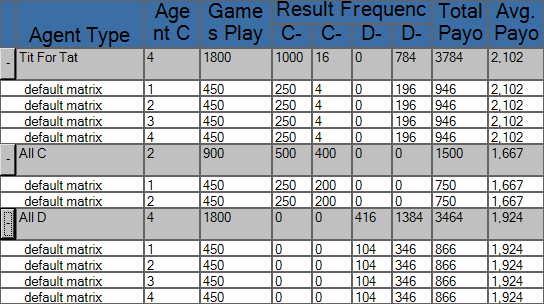
\includegraphics[width=.6\columnwidth]{../img/ipdmp/ipdmp10-table-det}
    \caption{10-players IPD, static strategies, software results \cite{demosw}}
    \label{fig:ipdmp10statsw}
\end{figure}

\begin{table}[ht]
    \caption{rMPIPD, constant pop. of 50, strategy evolution through repetitions}
    \label{tab:ripdmp-const}
    \centering
    \begin{tabular}{l|ccccc} \toprule
        $\downarrow$ Strategy -- Iter $\rightarrow$  & 0 & 1 & 2 & 3 & 4 \\ \midrule
        \textbf{GrimTrigger} &  5 &  5 &   9 &  17 &  30 \\
        TitFor2Tat        &  7 &  7 &   8 &   6 &   2 \\
        TitForTat         &  8 &  8 &  15 &  19 &  14 \\
        Nice              &  6 &  6 &   3 &   0 &   0 \\
        MainlyNice (k=3)  &  1 &  1 &   1 &   0 &   0 \\
        MainlyNice (k=8)  &  1 &  1 &   0 &   0 &   0 \\
        MainlyNice (k=17) &  1 &  1 &   0 &   0 &   0 \\
        MainlyNice (k=42) &  1 &  1 &   1 &   1 &   1 \\
        Indifferent       &  7 &  7 &   3 &   0 &   0 \\
        MainlyBad (k=70)  &  1 &  1 &   0 &   0 &   0 \\
        MainlyBad (k=78)  &  1 &  1 &   1 &   0 &   0 \\
        MainlyBad (k=81)  &  2 &  2 &   1 &   1 &   0 \\
        MainlyBad (k=85)  &  1 &  1 &   0 &   0 &   0 \\
        MainlyBad (k=97)  &  1 &  1 &   1 &   1 &   0 \\
        MainlyBad (k=98)  &  1 &  1 &   1 &   1 &   1 \\
        MainlyBad (k=99)  &  1 &  1 &   1 &   1 &   1 \\
        Bad               &  5 &  5 &   5 &   3 &   1 \\ \bottomrule
    \end{tabular}
\end{table}

\begin{table}[ht]
    \caption{rMPIPD, constant pop. of 50, $seed = 24$, strategy evolution}
    \label{tab:ripdmp-const-24}
    \centering
    \begin{tabular}{l|rrrrrrrr} \toprule
        $\downarrow$ Strategy -- Iter $\rightarrow$  & 0 & 1 & 2 & 3 & 4 & 5 & 6 & 7 \\ \midrule
        GrimTrigger       &   1 &   1 &   2 &   3 &   6 &  11 &  15 &  13 \\
        TitFor2Tat        &   5 &   5 &   3 &   2 &   0 &   0 &   0 &   0 \\
        \textbf{TitForTat}&   9 &   9 &  14 &  23 &  35 &  35 &  35 &  37 \\
        Nice              &   3 &   3 &   2 &   1 &   1 &   0 &   0 &   0 \\
        MainlyNice (k=4)  &   1 &   1 &   1 &   1 &   0 &   0 &   0 &   0 \\
        MainlyNice (k=5)  &   1 &   1 &   1 &   1 &   0 &   0 &   0 &   0 \\
        MainlyNice (k=28) &   1 &   1 &   1 &   1 &   0 &   0 &   0 &   0 \\
        MainlyNice (k=34) &   2 &   2 &   2 &   2 &   0 &   0 &   0 &   0 \\
        Indifferent       &   5 &   5 &   3 &   2 &   2 &   0 &   0 &   0 \\
        MainlyBad (k=51)  &   1 &   1 &   1 &   1 &   0 &   0 &   0 &   0 \\
        MainlyBad (k=52)  &   1 &   1 &   0 &   0 &   0 &   0 &   0 &   0 \\
        MainlyBad (k=56)  &   1 &   1 &   1 &   0 &   0 &   0 &   0 &   0 \\
        MainlyBad (k=58)  &   1 &   1 &   1 &   0 &   0 &   0 &   0 &   0 \\
        MainlyBad (k=61)  &   1 &   1 &   0 &   0 &   0 &   0 &   0 &   0 \\
        MainlyBad (k=70)  &   1 &   1 &   1 &   0 &   0 &   0 &   0 &   0 \\
        MainlyBad (k=92)  &   2 &   2 &   1 &   1 &   0 &   0 &   0 &   0 \\
        MainlyBad (k=93)  &   1 &   1 &   2 &   1 &   1 &   0 &   0 &   0 \\
        MainlyBad (k=96)  &   1 &   1 &   1 &   0 &   0 &   0 &   0 &   0 \\
        MainlyBad (k=97)  &   1 &   1 &   2 &   2 &   1 &   1 &   0 &   0 \\
        Bad               &  11 &  11 &  11 &   9 &   4 &   3 &   0 &   0 \\ \bottomrule
    \end{tabular}
\end{table}

\begin{table}[ht]
    \caption{rMPIPD, constant pop. of 50, $seed = 1209$, strategy evolution}
    \label{tab:ripdmp-const-1209}
    \centering
    \begin{tabular}{l|rrrrr} \toprule
        $\downarrow$ Strategy -- Iter $\rightarrow$  & 0 & 1 & 2 & 3 & 4 \\ \midrule
        GrimTrigger       &   1 &   1 &   1 &   2 &   3 \\
        TitFor2Tat        &   5 &   5 &   4 &   1 &   0 \\
        TitForTat         &   8 &   8 &   6 &   2 &   1 \\
        Nice              &   6 &   6 &   2 &   2 &   1 \\
        MainlyNice (k=4)  &   2 &   2 &   2 &   2 &   0 \\
        MainlyNice (k=12) &   1 &   1 &   1 &   1 &   0 \\
        MainlyNice (k=24) &   1 &   1 &   0 &   0 &   0 \\
        MainlyNice (k=31) &   1 &   1 &   1 &   0 &   0 \\
        MainlyNice (k=34) &   1 &   1 &   1 &   0 &   0 \\
        Indifferent       &  11 &  11 &   9 &   6 &   3 \\
        MainlyBad (k=58)  &   1 &   1 &   1 &   1 &   0 \\
        MainlyBad (k=63)  &   1 &   1 &   2 &   2 &   1 \\
        MainlyBad (k=74)  &   1 &   1 &   2 &   1 &   1 \\
        MainlyBad (k=76)  &   1 &   1 &   1 &   1 &   1 \\
        MainlyBad (k=82)  &   1 &   1 &   2 &   3 &   2 \\
        MainlyBad (k=99)  &   1 &   1 &   2 &   3 &   4 \\
        \textbf{Bad}      &   7 &   7 &  13 &  23 &  33 \\ \bottomrule
    \end{tabular}
\end{table}

\begin{table}[ht]
    \caption{rMPIPD, increasing pop. (alternative 1), strategy evolution through repetitions}
    \label{tab:ripdmp-incr}
    \centering
    \begin{tabular}{l|cccccc} \toprule
        $\downarrow$ Strategy -- Iter $\rightarrow$ & 0 & 1 & 2 & 3 & 4 & 5 \\ \midrule
        \textbf{GrimTrigger} &  5 &   9 &  18 &  35 &  66 &  125 \\
        TitFor2Tat           &  7 &  12 &  20 &  31 &  44 &   58 \\
        \textbf{TitForTat}   &  8 &  14 &  26 &  42 &  72 &  119 \\
        Nice                 &  6 &   6 &   8 &  12 &  18 &   23 \\
        MainlyNice (k=3)     &  1 &   1 &   1 &   1 &   1 &    2 \\
        MainlyNice (k=8)     &  1 &   1 &   1 &   2 &   4 &    5 \\
        MainlyNice (k=17)    &  1 &   1 &   1 &   1 &   1 &    1 \\
        MainlyNice (k=42)    &  1 &   2 &   3 &   5 &   6 &    8 \\
        Indifferent          &  7 &   7 &   9 &  10 &  11 &   13 \\
        MainlyBad (k=70)     &  1 &   1 &   2 &   3 &   4 &    4 \\
        MainlyBad (k=78)     &  1 &   2 &   3 &   4 &   4 &    4 \\
        MainlyBad (k=81)     &  2 &   3 &   4 &   5 &   6 &    7 \\
        MainlyBad (k=85)     &  1 &   1 &   1 &   1 &   1 &    1 \\
        MainlyBad (k=97)     &  1 &   1 &   1 &   1 &   1 &    1 \\
        MainlyBad (k=98)     &  1 &   1 &   1 &   1 &   1 &    1 \\
        MainlyBad (k=99)     &  1 &   2 &   2 &   2 &   2 &    2 \\
        Bad                  &  5 &   8 &   9 &  10 &  10 &   10 \\ \midrule
        Population size      & 50 &  72 & 110 & 166 & 252 &  384 \\ \bottomrule
    \end{tabular}
\end{table}

\begin{table}[ht]
    \caption{rMPIPD, increasing pop. (alternative 2), strategy evolution through repetitions}
    \label{tab:ripdmp-incrA2}
    \centering
    \begin{tabular}{l|cccccc} \toprule
        $\downarrow$ Strategy -- Iter $\rightarrow$ & 0 & 1 & 2 & 3 & 4 & 5 \\ \midrule
        \textbf{GrimTrigger} &   5 &   7 &   14 &   26 &   44 &   65 \\
        TitFor2Tat           &   7 &  12 &   17 &   22 &   27 &   34 \\
        \textbf{TitForTat}   &   8 &  14 &   24 &   35 &   42 &   51 \\
        Nice                 &   6 &   7 &    7 &    8 &    9 &   10 \\
        MainlyNice (k=3)     &   1 &   1 &    1 &    1 &    2 &    3 \\
        MainlyNice (k=8)     &   1 &   1 &    1 &    1 &    1 &    1 \\
        MainlyNice (k=17)    &   1 &   1 &    1 &    1 &    1 &    1 \\
        MainlyNice (k=42)    &   1 &   2 &    2 &    2 &    3 &    4 \\
        Indifferent          &   7 &   7 &    9 &   11 &   15 &   19 \\
        MainlyBad (k=70)     &   1 &   1 &    1 &    1 &    1 &    1 \\
        MainlyBad (k=78)     &   1 &   2 &    2 &    2 &    2 &    3 \\
        MainlyBad (k=81)     &   2 &   3 &    4 &    5 &    5 &    5 \\
        MainlyBad (k=85)     &   1 &   1 &    2 &    2 &    3 &    3 \\
        MainlyBad (k=97)     &   1 &   1 &    1 &    1 &    1 &    1 \\
        MainlyBad (k=98)     &   1 &   1 &    2 &    3 &    4 &    4 \\
        MainlyBad (k=99)     &   1 &   2 &    2 &    3 &    4 &    4 \\
        Bad                  &   5 &   9 &   11 &   13 &   15 &   19 \\ \midrule
        Population size      &  50 &  72 &  101 &  137 &  179 &  228 \\ \bottomrule
    \end{tabular}
\end{table}

\begin{figure}
    \centering
    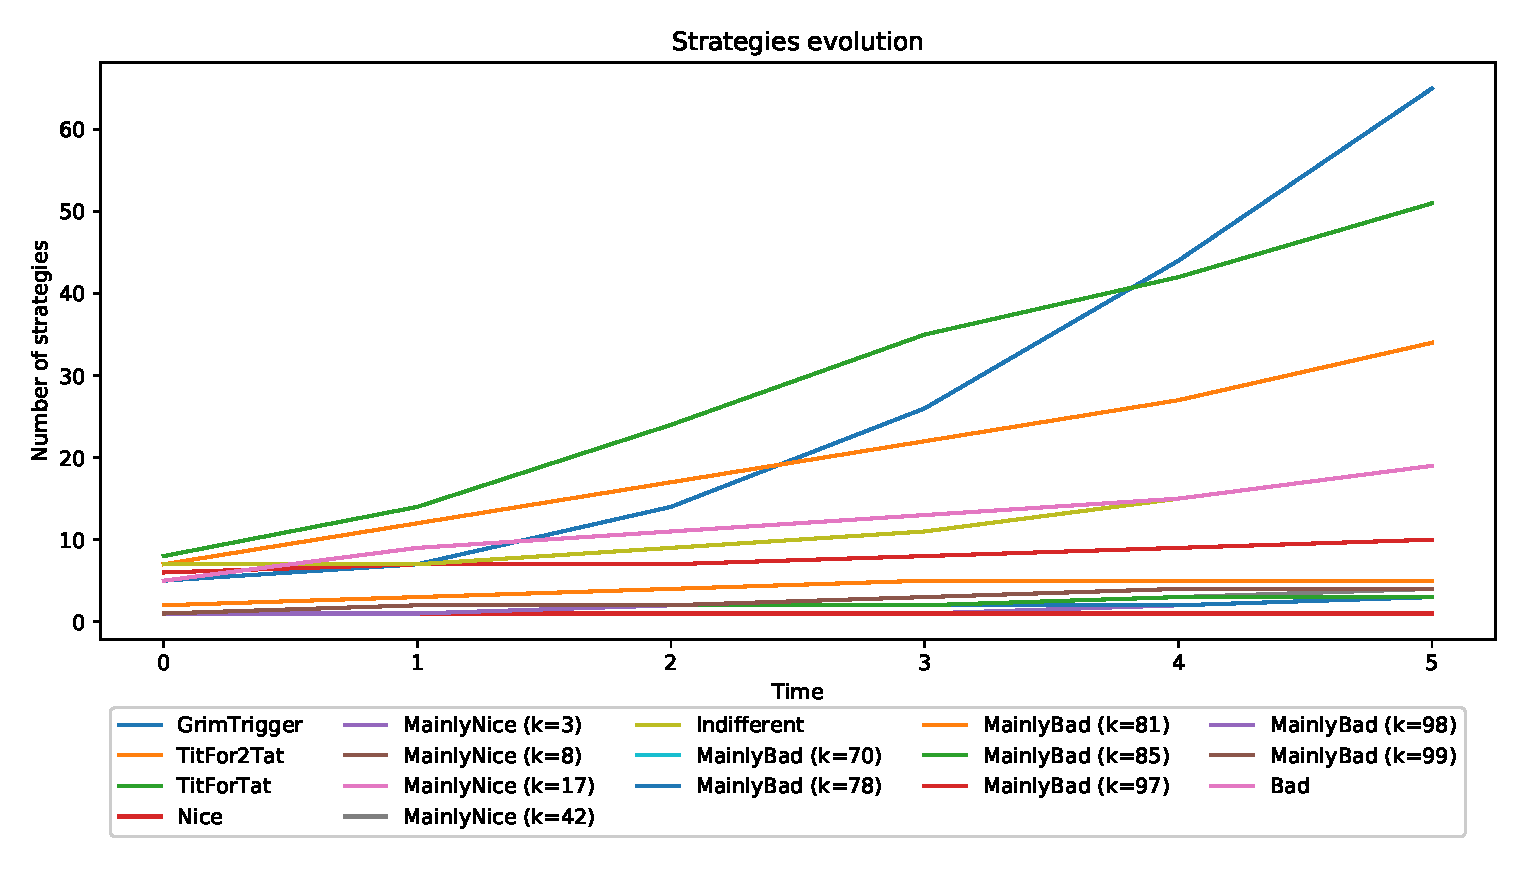
\includegraphics[width=.7\columnwidth]{../img/ripdmp-incr/alt2/ripdmp-evolution-increasing-pop-50}
    \caption{Evolution of rIPDMP, increasing population, from 50 (alternative 2)}
    \label{fig:incrRa2}
\end{figure}

%\begin{figure}
%    \centering
%    \includegraphics[width=.7\columnwidth]{../img/ripdmp-incr/alt2/ripdmp-scores-increasing-pop-50-r0}
%    \caption{First iteration scores ($it=0$) (alternative 2)}
%    \label{fig:incrFIa2}
%\end{figure}

%\begin{figure}
%    \centering
%    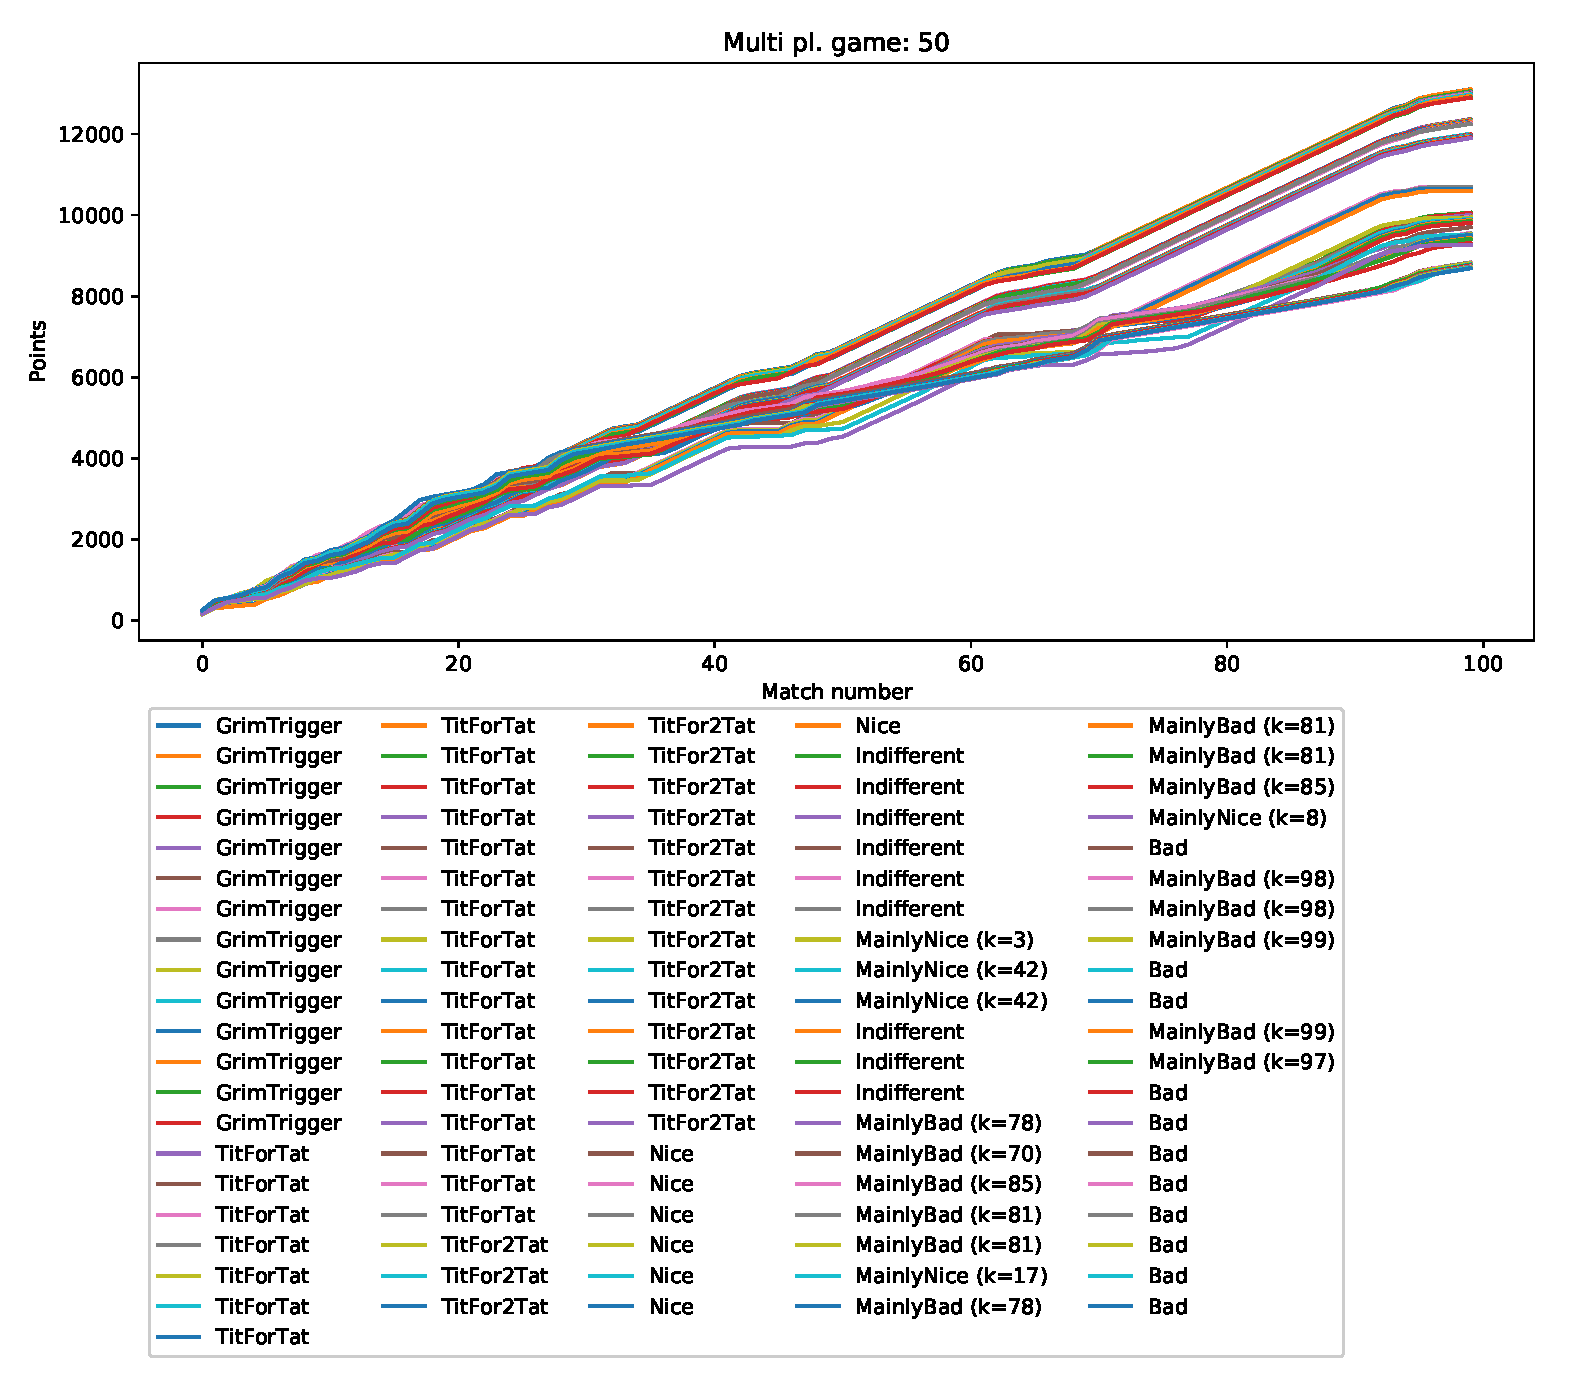
\includegraphics[width=.7\columnwidth]{../img/ripdmp-incr/alt2/ripdmp-scores-increasing-pop-50-r2}
%    \caption{Middle iteration scores ($it=2$) (alternative 2)}
%    \label{fig:incrMIa2}
%\end{figure}

%\begin{figure}
%    \centering
%    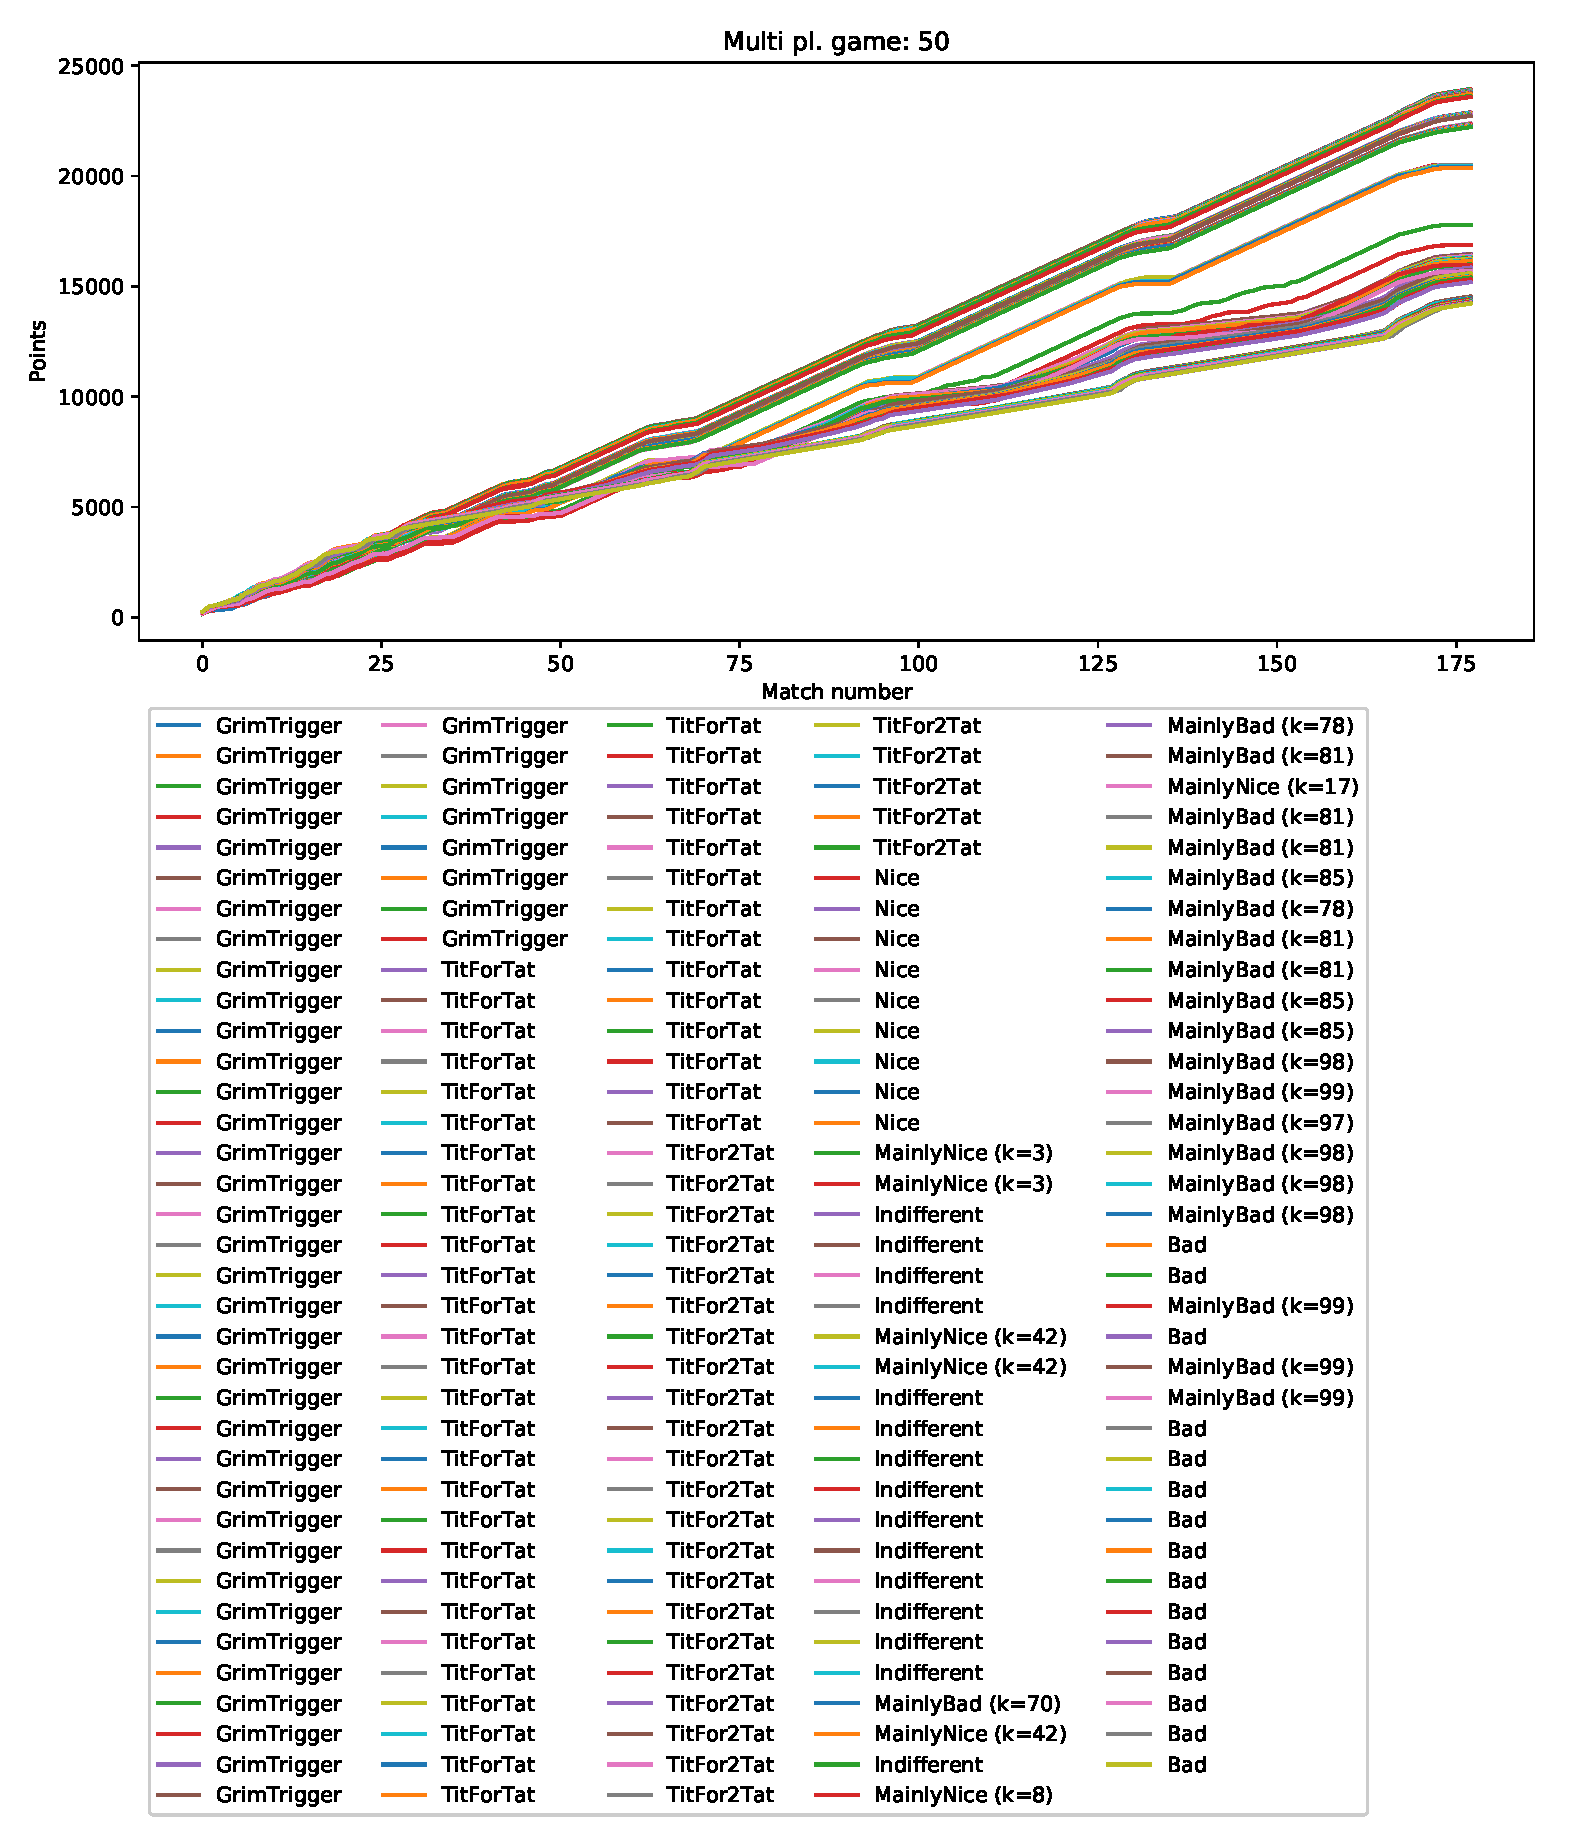
\includegraphics[width=.7\columnwidth]{../img/ripdmp-incr/alt2/ripdmp-scores-increasing-pop-50-r4}
%    \caption{Last iteration scores ($it=4$) (alternative 2)}
%    \label{fig:incrLIa2}
%\end{figure}

\begin{table}[ht]
    \caption{rMPIPD, increasing pop. (alternative 3), strategy evolution through repetitions}
    \label{tab:ripdmp-incrA3}
    \centering
    \begin{tabular}{l|cccccc} \toprule
        $\downarrow$ Strategy -- Iter $\rightarrow$ & 0 & 1 & 2 & 3 & 4 & 5 \\ \midrule
        GrimTrigger         &   5 &   7 &   10 &   12 &   16 &   18 \\
        \textbf{TitFor2Tat} &   7 &  14 &   26 &   42 &   70 &  113 \\
        \textbf{TitForTat}  &   8 &  16 &   32 &   64 &  128 &  256 \\
        Nice                &   6 &  11 &   20 &   31 &   42 &   56 \\
        MainlyNice (k=3)    &   1 &   1 &    1 &    1 &    1 &    1 \\
        MainlyNice (k=8)    &   1 &   1 &    1 &    1 &    1 &    1 \\
        MainlyNice (k=17)   &   1 &   1 &    1 &    1 &    1 &    1 \\
        MainlyNice (k=42)   &   1 &   1 &    1 &    1 &    1 &    1 \\
        Indifferent         &   7 &  11 &   17 &   26 &   31 &   36 \\
        MainlyBad (k=70)    &   1 &   1 &    1 &    1 &    1 &    1 \\
        MainlyBad (k=78)    &   1 &   1 &    1 &    1 &    1 &    1 \\
        MainlyBad (k=81)    &   2 &   2 &    2 &    2 &    2 &    2 \\
        MainlyBad (k=85)    &   1 &   1 &    1 &    1 &    1 &    1 \\
        MainlyBad (k=97)    &   1 &   1 &    1 &    1 &    1 &    1 \\
        MainlyBad (k=98)    &   1 &   1 &    1 &    1 &    1 &    1 \\
        MainlyBad (k=99)    &   1 &   1 &    1 &    1 &    1 &    1 \\
        Bad                 &   5 &  10 &   16 &   21 &   26 &   32 \\ \midrule
        Population size     &  50 &  81 &  133 &  208 &  325 &  523 \\ \bottomrule
    \end{tabular}
\end{table}

\begin{figure}
    \centering
    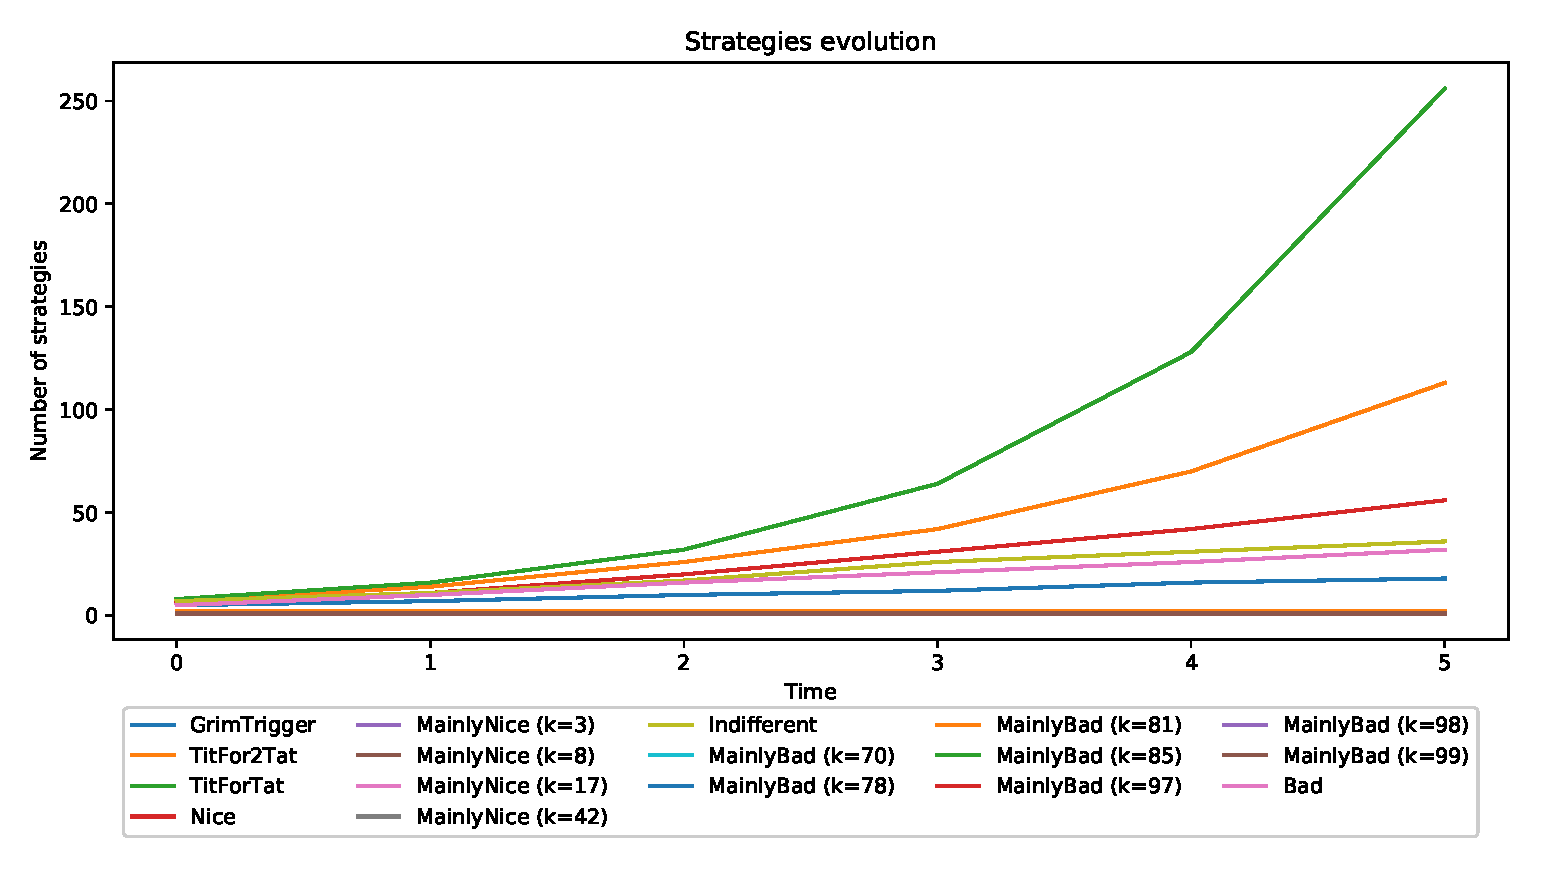
\includegraphics[width=.7\columnwidth]{../img/ripdmp-incr/alt3/ripdmp-evolution-increasing-pop-50}
    \caption{Evolution of rIPDMP, increasing population, from 50 (alternative 3)}
    \label{fig:incrRa3}
\end{figure}

%\begin{figure}
%    \centering
%    \includegraphics[width=.7\columnwidth]{../img/ripdmp-incr/alt3/ripdmp-scores-increasing-pop-50-r0}
%    \caption{First iteration scores ($it=0$) (alternative 3)}
%    \label{fig:incrFIa3}
%\end{figure}

%\begin{figure}
%    \centering
%    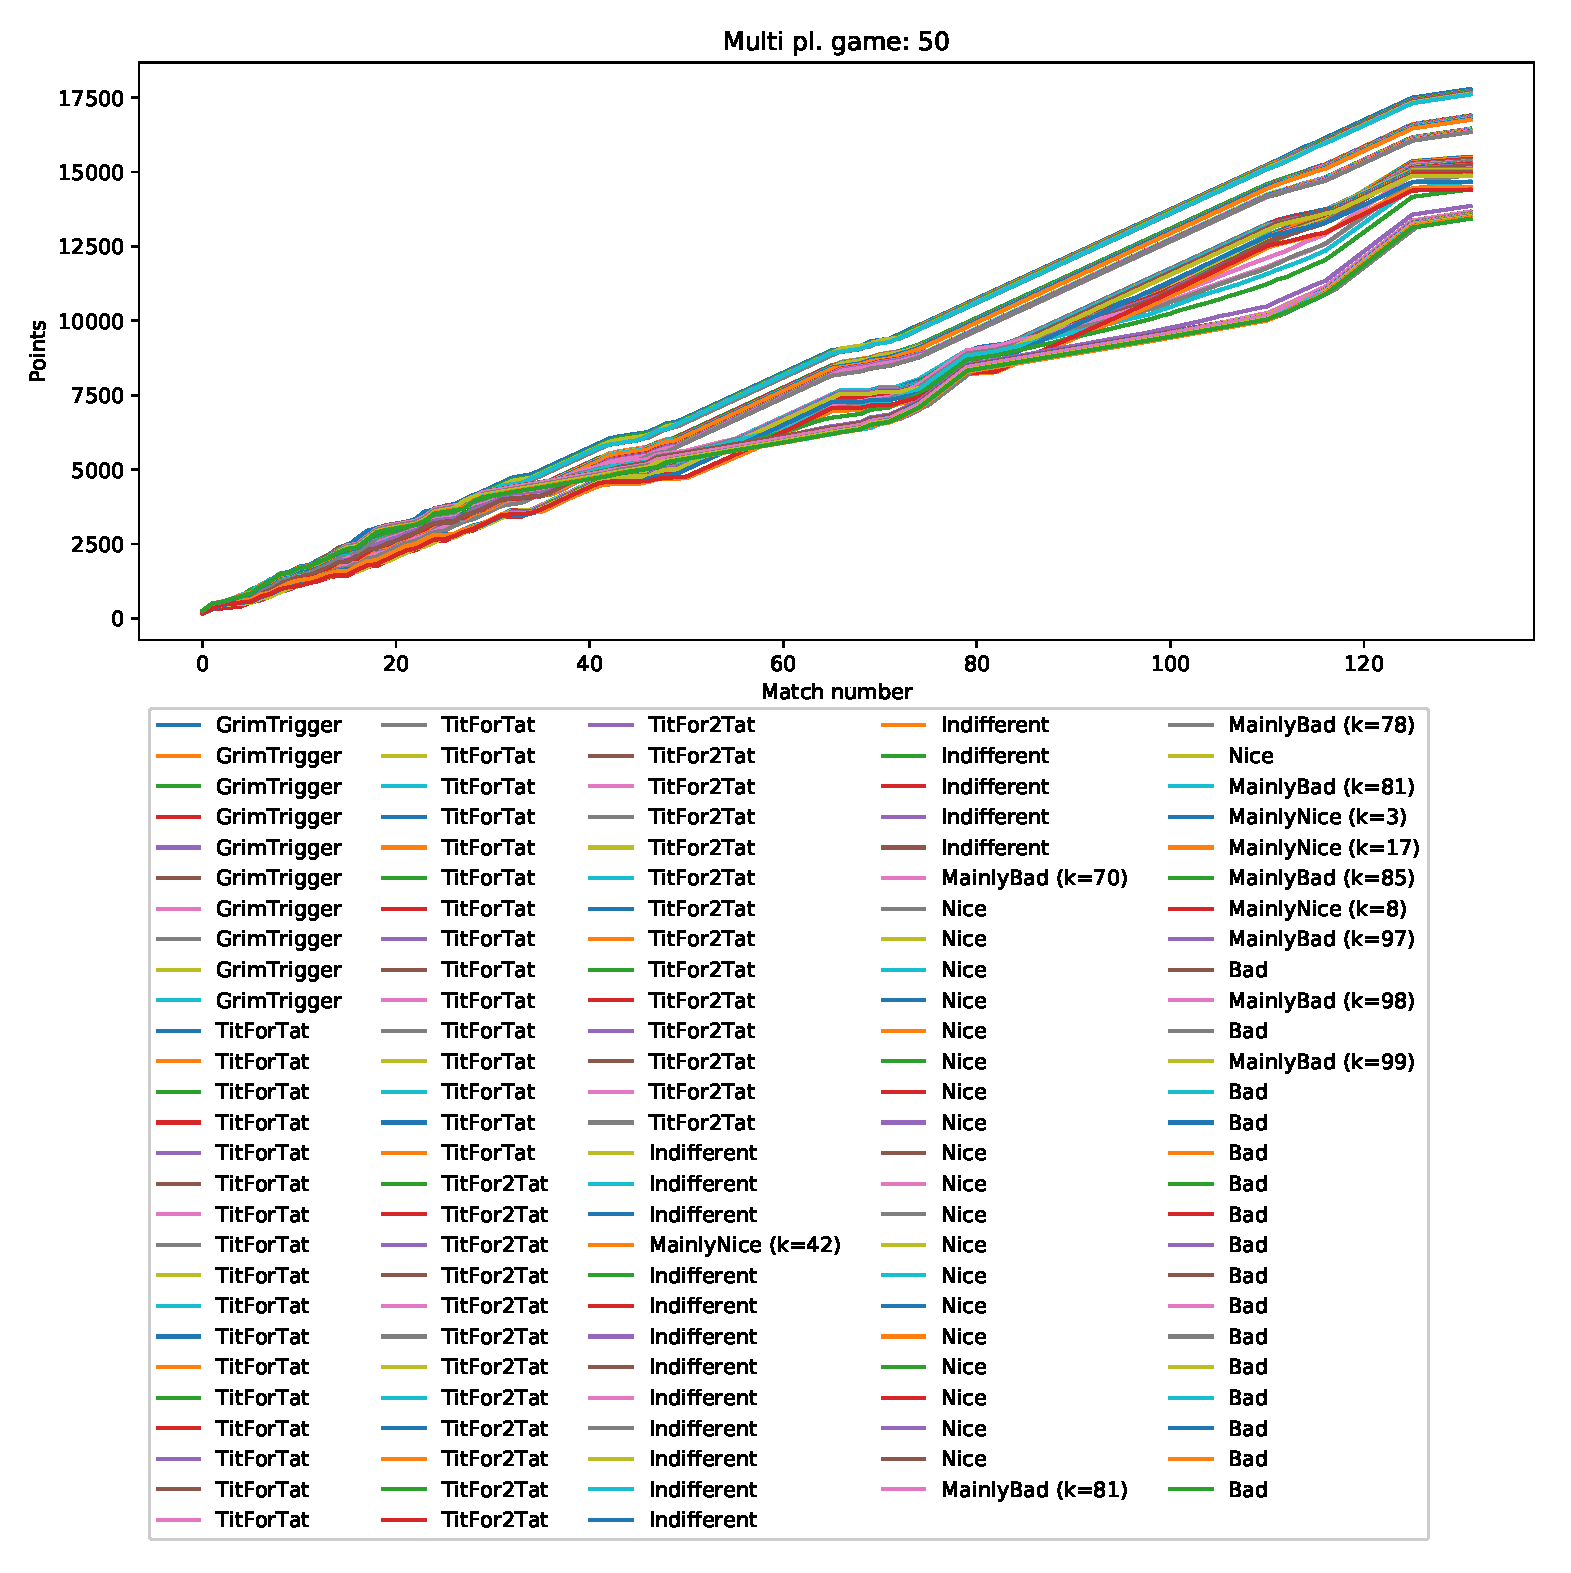
\includegraphics[width=.7\columnwidth]{../img/ripdmp-incr/alt3/ripdmp-scores-increasing-pop-50-r2}
%    \caption{Middle iteration scores ($it=2$) (alternative 3)}
%    \label{fig:incrMIa3}
%\end{figure}

%\begin{figure}
%    \centering
%    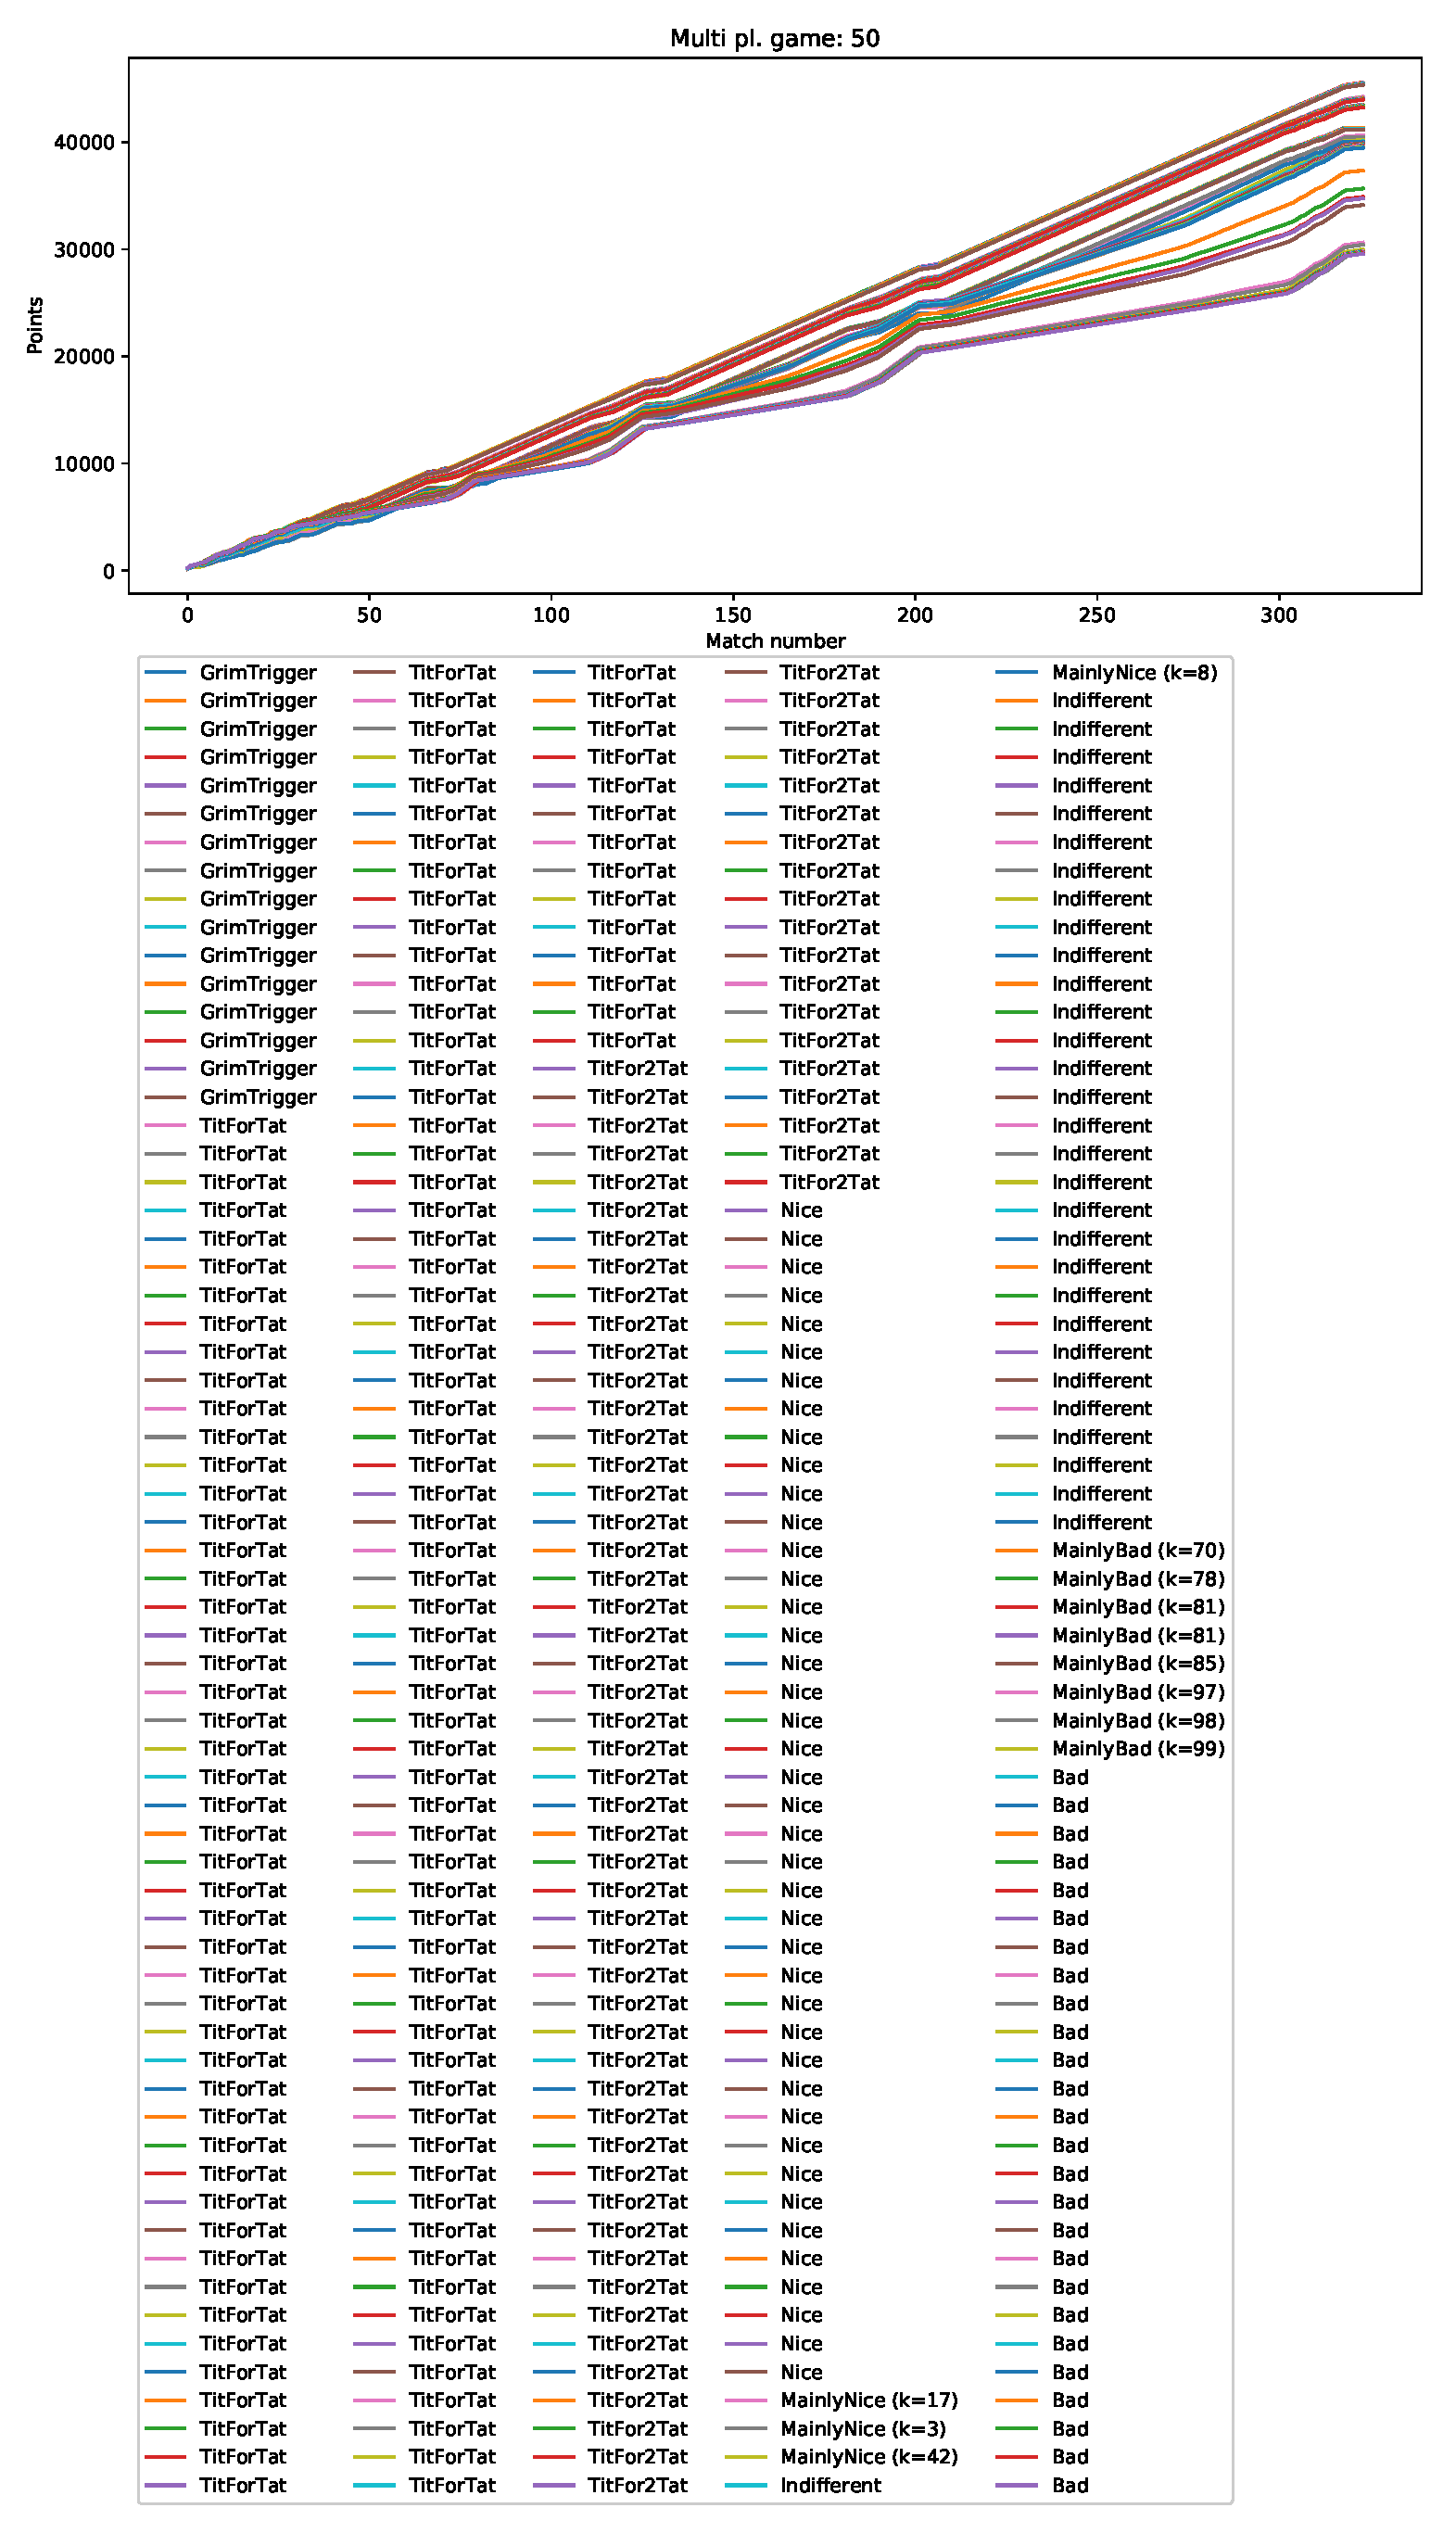
\includegraphics[width=.7\columnwidth]{../img/ripdmp-incr/alt3/ripdmp-scores-increasing-pop-50-r4}
%    \caption{Last iteration scores ($it=4$) (alternative 3)}
%    \label{fig:incrLIa3}
%\end{figure}

\begin{table}[ht]
    \caption{rMPIPD, changing strategies (alternative 1), strategy evolution through repetitions.\\
    Blank cell means player not present. At the end, strategy changes count for each iteration.}
    \label{tab:cripdmp}
    \centering
    \begin{minipage}{.4\textwidth}
    \begin{tabular}{l|cccccc} \toprule
        $\downarrow$ Strategy -- Iter $\rightarrow$ & 0 & 1 & 2 & 3 & 4 & 5 \\ \midrule
        \textbf{GrimTrigger} &   5 &   9 &   15 &   22 &   31 &   41 \\
        \textbf{TitFor2Tat}  &   7 &  12 &   17 &   23 &   34 &   50 \\
        \textbf{TitForTat}   &   8 &  14 &   16 &   20 &   32 &   56 \\
        Nice                 &   6 &   6 &    8 &    9 &   12 &   13 \\
        MainlyNice (k=3)     &   1 &   1 &    1 &    1 &    1 &    1 \\
        MainlyNice (k=8)     &   1 &   1 &    1 &    1 &    1 &    1 \\
        MainlyNice (k=17)    &   1 &   1 &    1 &    2 &    2 &    2 \\
        MainlyNice (k=42)    &   1 &   2 &    3 &    6 &    9 &   12 \\
        Indifferent          &   7 &   7 &    9 &   11 &   12 &   14 \\
        MainlyBad (k=70)     &   1 &   1 &    1 &    1 &    3 &    4 \\
        MainlyBad (k=78)     &   1 &   2 &    2 &    2 &    3 &    3 \\
        MainlyBad (k=81)     &   2 &   3 &    4 &    5 &    5 &    5 \\
        MainlyBad (k=85)     &   1 &   1 &    1 &    2 &    3 &    3 \\
        MainlyBad (k=97)     &   1 &   1 &    1 &    1 &    1 &    1 \\
        MainlyBad (k=98)     &   1 &   1 &    1 &    1 &    1 &    1 \\
        MainlyBad (k=99)     &   1 &   2 &    2 &    2 &    2 &    2 \\
        Bad                  &   5 &   8 &   10 &   11 &   12 &   13 \\
        MainlyNice (k=11)    &     &     &    1 &    2 &    2 &    2 \\
        MainlyNice (k=20)    &     &     &    1 &    2 &    3 &    4 \\
        MainlyNice (k=24)    &     &     &    1 &    1 &    2 &    2 \\
        MainlyNice (k=29)    &     &     &    1 &    1 &    1 &    1 \\
        MainlyNice (k=38)    &     &     &    1 &    2 &    2 &    3 \\
        MainlyNice (k=40)    &     &     &    1 &    3 &    5 &    8 \\
        MainlyNice (k=43)    &     &     &    1 &    1 &    1 &    3 \\
        MainlyBad (k=51)     &     &     &    1 &    3 &    5 &    6 \\
        MainlyBad (k=56)     &     &     &    1 &    2 &    3 &    4 \\
        MainlyBad (k=62)     &     &     &    1 &    2 &    2 &    3 \\
        MainlyBad (k=63)     &     &     &    1 &    2 &    4 &    4 \\
        MainlyBad (k=68)     &     &     &    1 &    1 &    1 &    5 \\
        MainlyBad (k=69)     &     &     &    1 &    3 &    4 &    5 \\
        MainlyBad (k=76)     &     &     &    1 &    1 &    1 &    1 \\
        MainlyBad (k=87)     &     &     &    1 &    1 &    3 &    4 \\
        MainlyNice (k=25)    &     &     &      &    1 &    1 &    1 \\
        MainlyNice (k=27)    &     &     &      &    1 &    1 &    2 \\
        MainlyNice (k=28)    &     &     &      &    1 &    1 &    1 \\
        MainlyNice (k=30)    &     &     &      &    1 &    1 &    2 \\
        MainlyNice (k=32)    &     &     &      &    1 &    1 &    4 \\
        MainlyNice (k=35)    &     &     &      &    1 &    1 &    2 \\
        MainlyNice (k=36)    &     &     &      &    1 &    2 &    2 \\
        MainlyBad (k=52)     &     &     &      &    1 &    2 &    2 \\
        MainlyBad (k=55)     &     &     &      &    1 &    2 &    2 \\
        MainlyBad (k=59)     &     &     &      &    1 &    3 &    4 \\
        MainlyBad (k=60)     &     &     &      &    1 &    2 &    5 \\
        MainlyBad (k=61)     &     &     &      &    1 &    4 &    7 \\
        MainlyBad (k=71)     &     &     &      &    1 &    1 &    1 \\
        MainlyBad (k=72)     &     &     &      &    1 &    1 &    1 \\
        MainlyBad (k=84)     &     &     &      &    1 &    1 &    2 \\
        MainlyBad (k=86)     &     &     &      &    2 &    4 &    4 \\ \bottomrule
    \end{tabular}
    \end{minipage} \quad
    \begin{minipage}{.4\textwidth}
    \begin{tabular}{l|cccccc} \toprule
        $\downarrow$ Strategy -- Iter $\rightarrow$ & 0 & 1 & 2 & 3 & 4 & 5 \\ \midrule
        MainlyNice (k=7)     &     &     &      &      &    1 &    1 \\
        MainlyNice (k=23)    &     &     &      &      &    1 &    3 \\
        MainlyNice (k=34)    &     &     &      &      &    1 &    2 \\
        MainlyNice (k=37)    &     &     &      &      &    2 &    3 \\
        MainlyNice (k=39)    &     &     &      &      &    3 &    4 \\
        MainlyNice (k=46)    &     &     &      &      &    1 &    2 \\
        MainlyNice (k=47)    &     &     &      &      &    2 &    5 \\
        MainlyNice (k=49)    &     &     &      &      &    3 &    8 \\
        MainlyBad (k=54)     &     &     &      &      &    1 &    1 \\
        MainlyBad (k=66)     &     &     &      &      &    1 &    2 \\
        MainlyBad (k=67)     &     &     &      &      &    1 &    1 \\
        MainlyBad (k=73)     &     &     &      &      &    2 &    2 \\
        MainlyBad (k=74)     &     &     &      &      &    1 &    1 \\
        MainlyBad (k=77)     &     &     &      &      &    1 &    3 \\
        MainlyBad (k=80)     &     &     &      &      &    1 &    2 \\
        MainlyBad (k=90)     &     &     &      &      &    1 &    2 \\
        MainlyBad (k=94)     &     &     &      &      &    1 &    1 \\
        MainlyBad (k=95)     &     &     &      &      &    2 &    4 \\
        MainlyNice (k=22)    &     &     &      &      &      &    1 \\
        MainlyNice (k=26)    &     &     &      &      &      &    1 \\
        MainlyNice (k=31)    &     &     &      &      &      &    1 \\
        MainlyNice (k=33)    &     &     &      &      &      &    1 \\
        MainlyNice (k=41)    &     &     &      &      &      &    1 \\
        MainlyNice (k=44)    &     &     &      &      &      &    2 \\
        MainlyNice (k=45)    &     &     &      &      &      &    1 \\
        MainlyNice (k=48)    &     &     &      &      &      &    1 \\
        MainlyBad (k=57)     &     &     &      &      &      &    1 \\
        MainlyBad (k=64)     &     &     &      &      &      &    1 \\
        MainlyBad (k=65)     &     &     &      &      &      &    3 \\
        MainlyBad (k=82)     &     &     &      &      &      &    1 \\
        MainlyBad (k=88)     &     &     &      &      &      &    1 \\ \midrule
        Population size      &  50 &  72 &  108 &  164 &  257 &  385 \\
        To more cooperative  &  19 &  27 &   46 &   70 &  105 &  139 \\
        To less cooperative  &  19 &  26 &   46 &   63 &  101 &  160 \\ \bottomrule
    \end{tabular}
    \end{minipage}
\end{table}

\begin{table}[ht]
    \caption{rMPIPD, changing strategies (alternative 2), strategy evolution through repetitions.\\
    Blank cell means player not present. At the end, strategy changes count for each iteration.}
    \label{tab:cripdmpA2}
    \centering
    \begin{minipage}{.4\textwidth}
    \begin{tabular}{l|cccccc} \toprule
        $\downarrow$ Strategy -- Iter $\rightarrow$ & 0 & 1 & 2 & 3 & 4 & 5 \\ \midrule
        GrimTrigger         &   5 &   9 &   12 &   18 &   21 &   27 \\
        \textbf{TitFor2Tat} &   7 &  12 &   23 &   32 &   36 &   38 \\
        \textbf{TitForTat}  &   8 &  14 &   22 &   26 &   34 &   44 \\
        Nice                &   6 &   6 &    9 &    9 &   10 &   10 \\
        MainlyNice (k=3)    &   1 &   1 &    1 &    1 &    1 &    1 \\
        MainlyNice (k=8)    &   1 &   1 &    1 &    1 &    1 &    1 \\
        MainlyNice (k=17)   &   1 &   1 &    1 &    1 &    1 &    1 \\
        MainlyNice (k=42)   &   1 &   2 &    2 &    3 &    4 &    5 \\
        Indifferent         &   7 &   7 &    7 &    9 &   12 &   18 \\
        MainlyBad (k=70)    &   1 &   1 &    1 &    2 &    3 &    4 \\
        MainlyBad (k=78)    &   1 &   2 &    2 &    2 &    3 &    4 \\
        MainlyBad (k=81)    &   2 &   3 &    4 &    6 &    8 &   10 \\
        MainlyBad (k=85)    &   1 &   1 &    1 &    2 &    4 &    5 \\
        MainlyBad (k=97)    &   1 &   1 &    2 &    3 &    5 &    6 \\
        MainlyBad (k=98)    &   1 &   1 &    1 &    1 &    1 &    1 \\
        MainlyBad (k=99)    &   1 &   2 &    2 &    2 &    2 &    2 \\
        \textbf{Bad}        &   5 &   8 &    9 &   14 &   25 &   41 \\
        MainlyNice (k=34)   &     &     &    1 &    2 &    2 &    4 \\
        MainlyNice (k=35)   &     &     &    1 &    1 &    4 &    6 \\
        MainlyNice (k=36)   &     &     &    1 &    2 &    5 &    8 \\
        MainlyNice (k=44)   &     &     &    1 &    2 &    3 &    4 \\
        MainlyNice (k=48)   &     &     &    2 &    2 &    4 &    7 \\
        MainlyBad (k=57)    &     &     &    1 &    2 &    4 &    8 \\
        MainlyBad (k=60)    &     &     &    1 &    2 &    3 &    5 \\
        MainlyBad (k=61)    &     &     &    1 &    1 &    2 &    4 \\
        MainlyBad (k=71)    &     &     &    1 &    2 &    4 &    5 \\
        MainlyNice (k=30)   &     &     &      &    1 &    2 &    2 \\
        MainlyNice (k=39)   &     &     &      &    3 &    5 &    8 \\
        MainlyNice (k=41)   &     &     &      &    1 &    2 &    3 \\
        MainlyNice (k=43)   &     &     &      &    1 &    2 &    3 \\
        MainlyNice (k=45)   &     &     &      &    1 &    3 &    5 \\
        MainlyNice (k=47)   &     &     &      &    1 &    2 &    4 \\ \bottomrule
    \end{tabular}
    \end{minipage} \quad
    \begin{minipage}{.4\textwidth}
    \begin{tabular}{l|cccccc} \toprule
        $\downarrow$ Strategy -- Iter $\rightarrow$ & 0 & 1 & 2 & 3 & 4 & 5 \\ \midrule
        MainlyBad (k=55)    &     &     &      &    1 &    1 &    1 \\
        MainlyBad (k=56)    &     &     &      &    1 &    2 &    8 \\
        MainlyBad (k=62)    &     &     &      &    1 &    2 &    5 \\
        MainlyBad (k=64)    &     &     &      &    1 &    3 &    6 \\
        MainlyBad (k=72)    &     &     &      &    1 &    4 &    6 \\
        MainlyNice (k=37)   &     &     &      &      &    1 &    2 \\
        MainlyNice (k=38)   &     &     &      &      &    1 &    2 \\
        MainlyNice (k=46)   &     &     &      &      &    1 &    3 \\
        MainlyNice (k=49)   &     &     &      &      &    1 &    2 \\
        MainlyBad (k=52)    &     &     &      &      &    1 &    6 \\
        MainlyBad (k=53)    &     &     &      &      &    3 &    6 \\
        MainlyBad (k=54)    &     &     &      &      &    1 &    2 \\
        MainlyBad (k=58)    &     &     &      &      &    1 &    1 \\
        MainlyBad (k=59)    &     &     &      &      &    1 &    3 \\
        MainlyBad (k=67)    &     &     &      &      &    1 &    5 \\
        MainlyBad (k=68)    &     &     &      &      &    1 &    4 \\
        MainlyBad (k=69)    &     &     &      &      &    1 &    2 \\
        MainlyBad (k=74)    &     &     &      &      &    1 &    2 \\
        MainlyNice (k=20)   &     &     &      &      &      &    1 \\
        MainlyNice (k=27)   &     &     &      &      &      &    1 \\
        MainlyBad (k=51)    &     &     &      &      &      &    2 \\
        MainlyBad (k=63)    &     &     &      &      &      &    1 \\
        MainlyBad (k=65)    &     &     &      &      &      &    2 \\
        MainlyBad (k=66)    &     &     &      &      &      &    3 \\
        MainlyBad (k=75)    &     &     &      &      &      &    1 \\
        MainlyBad (k=77)    &     &     &      &      &      &    1 \\
        MainlyBad (k=80)    &     &     &      &      &      &    1 \\ \midrule
        Population size     &  50 &  72 &  110 &  161 &  245 &  373 \\
        To more cooperative &  11 &  16 &   19 &   19 &   39 &   72 \\
        To less cooperative &  11 &  24 &   38 &   55 &   63 &   93 \\ \bottomrule
    \end{tabular}
    \end{minipage}
\end{table}

\begin{figure}[!ht]
    \centering
    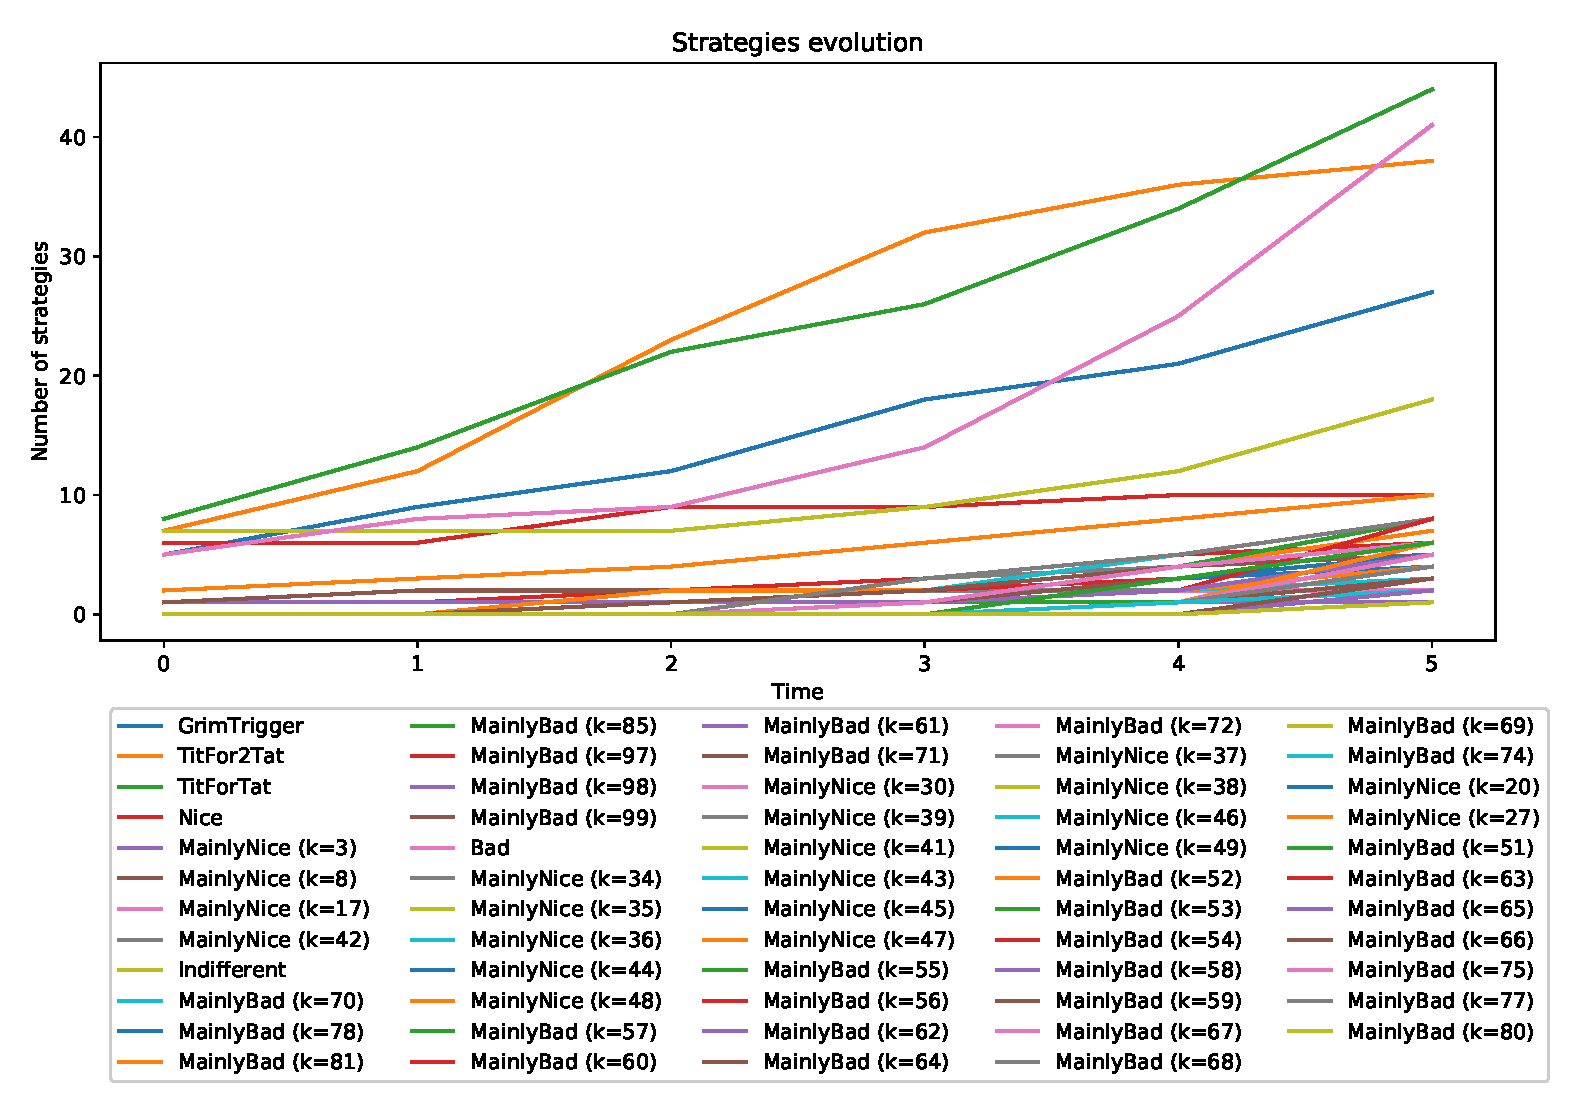
\includegraphics[width=.8\columnwidth]{../img/cipdmp-incr/alt2/cipdmp-evolution-increasing-pop-50}
    \caption{Evolution of rIPDMP, changing strategies, increasing pop. from 50 (alternative 2)}
    \label{fig:incrC2}
\end{figure}

%\begin{figure}[!ht]
%    \centering
%    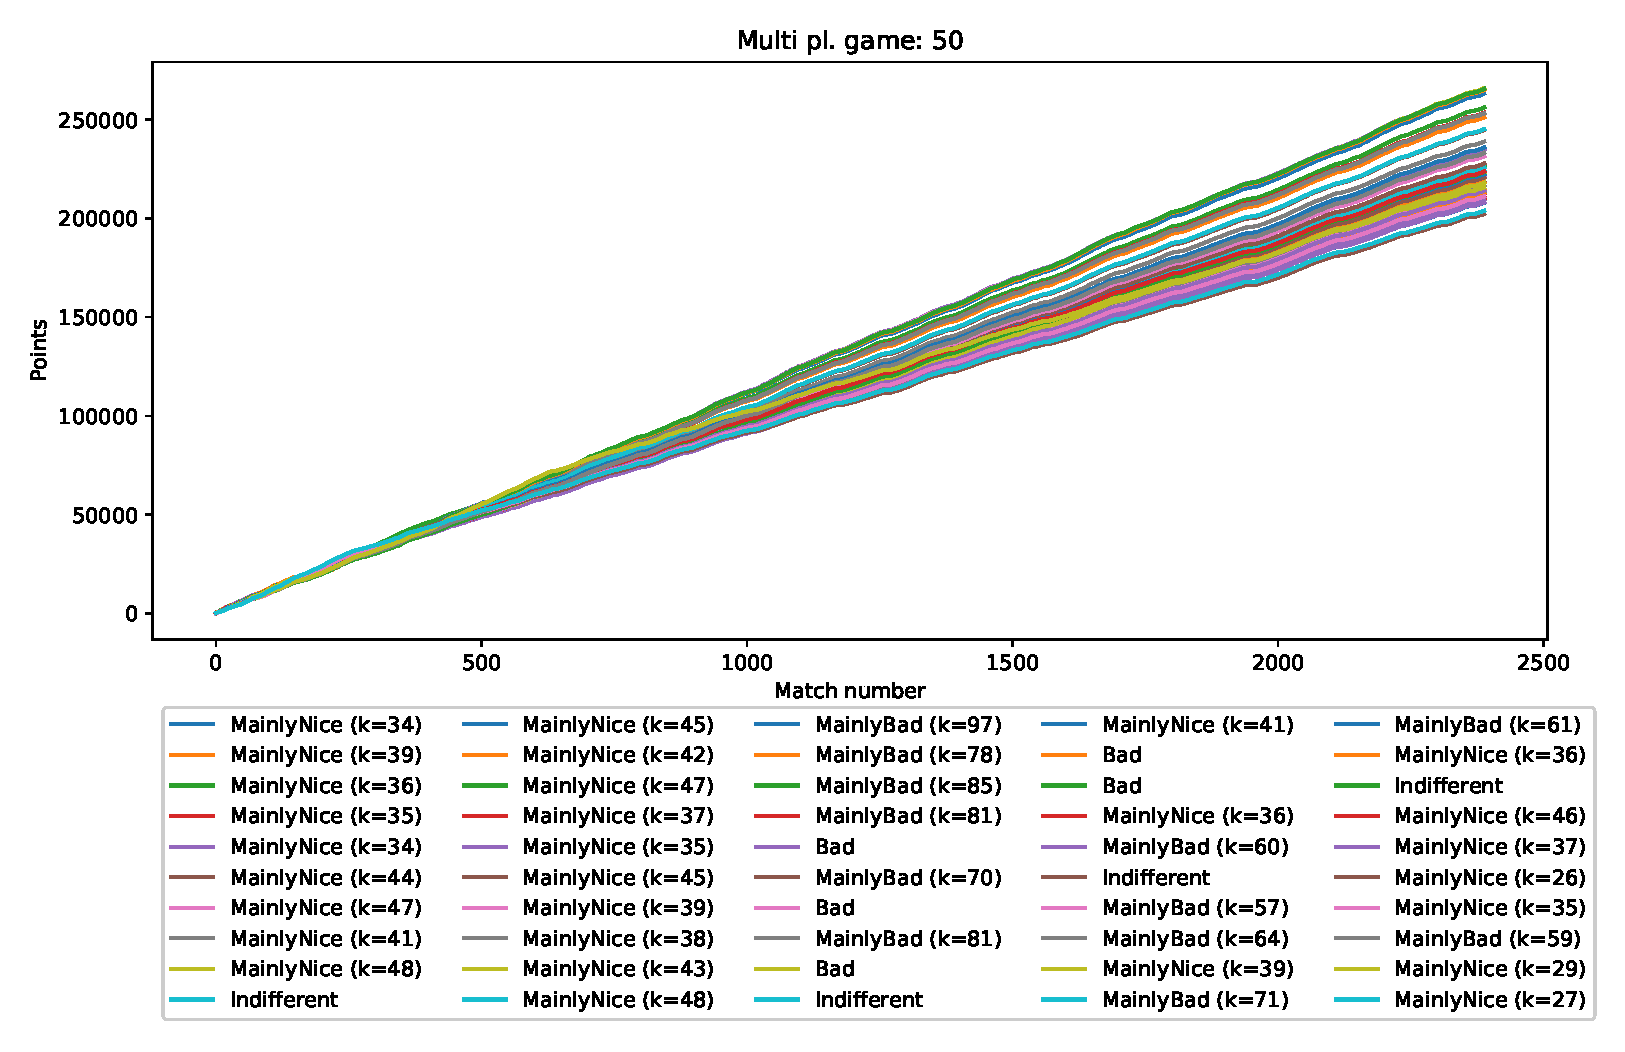
\includegraphics[width=.7\columnwidth]{../img/cipdmp-incr/alt2/cipdmp-scores-increasing-pop-50-r0}
%    \caption{First iteration scores ($it=0$) (alternative 2)}
%    \label{fig:incrCFI2}
%\end{figure}

%\begin{figure}[!ht]
%    \centering
%    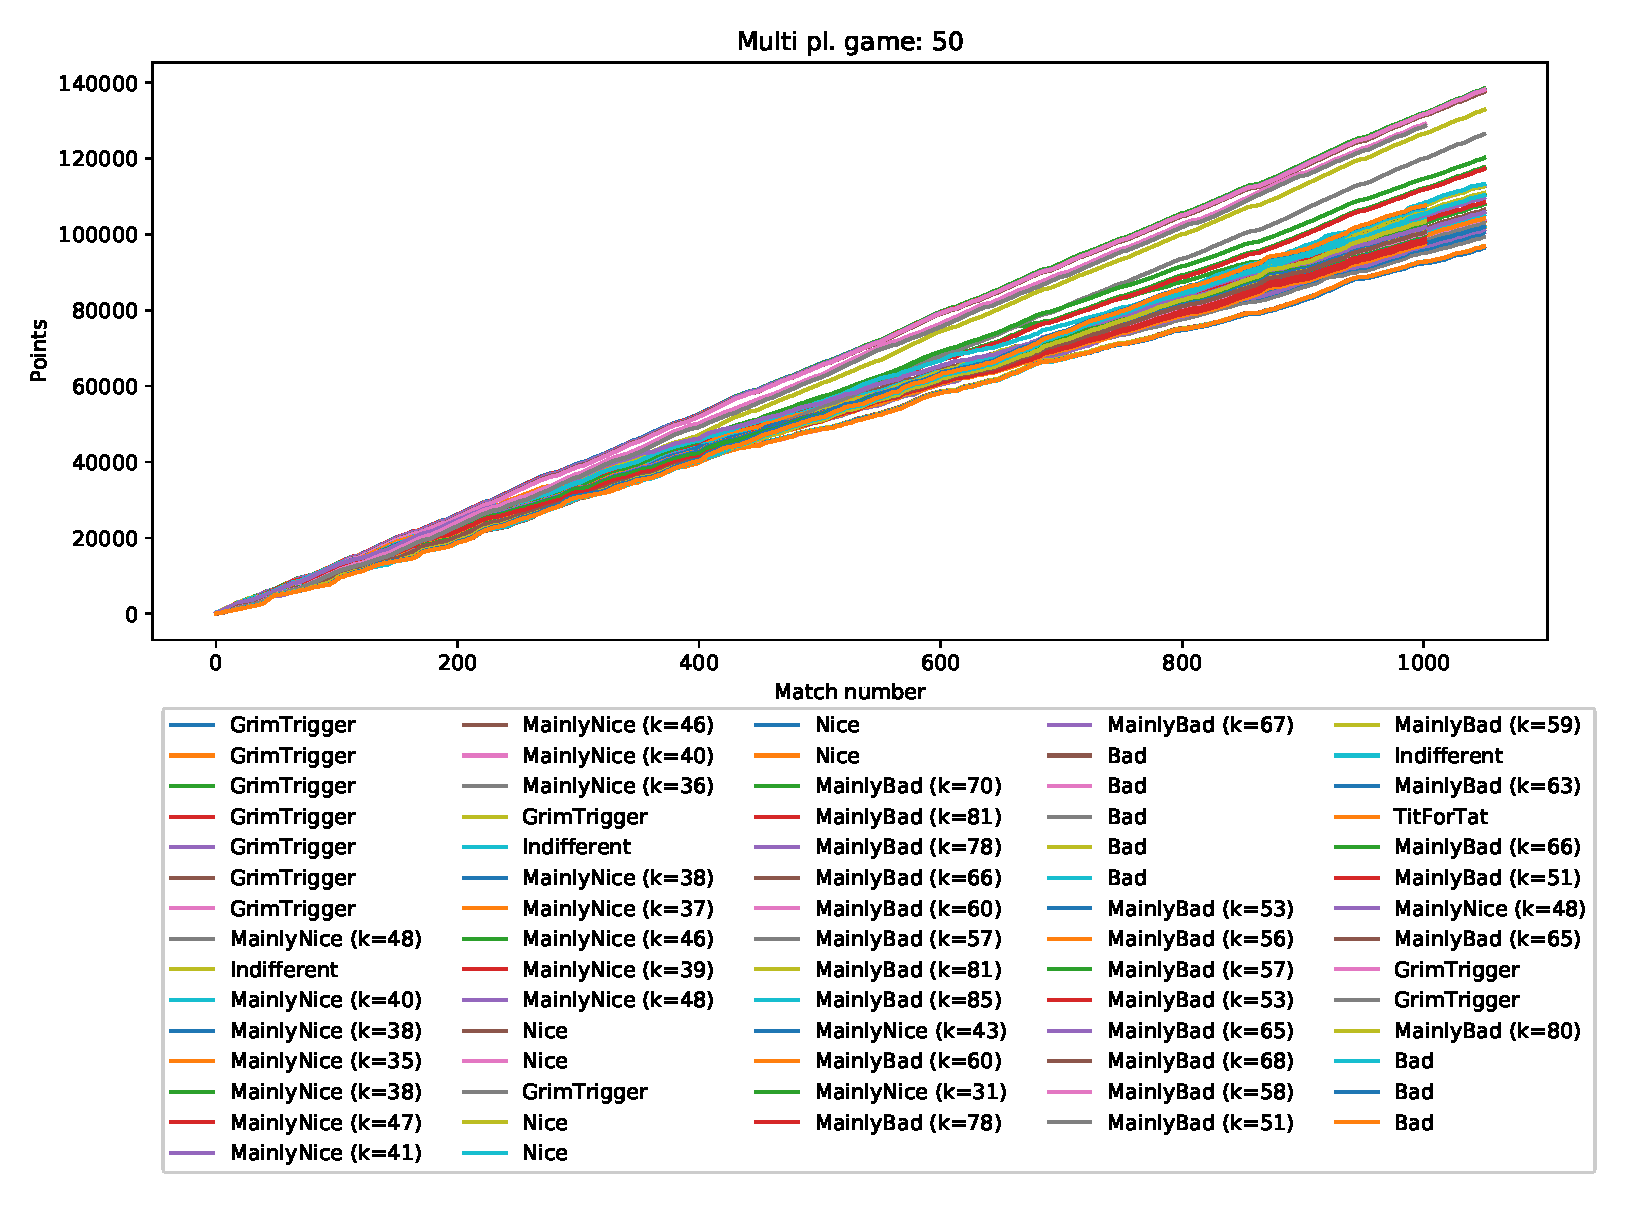
\includegraphics[width=.7\columnwidth]{../img/cipdmp-incr/alt2/cipdmp-scores-increasing-pop-50-r2}
%    \caption{Middle iteration scores ($it=2$) (alternative 2)}
%    \label{fig:incrCMI2}
%\end{figure}

%\begin{figure}[!ht]
%    \centering
%    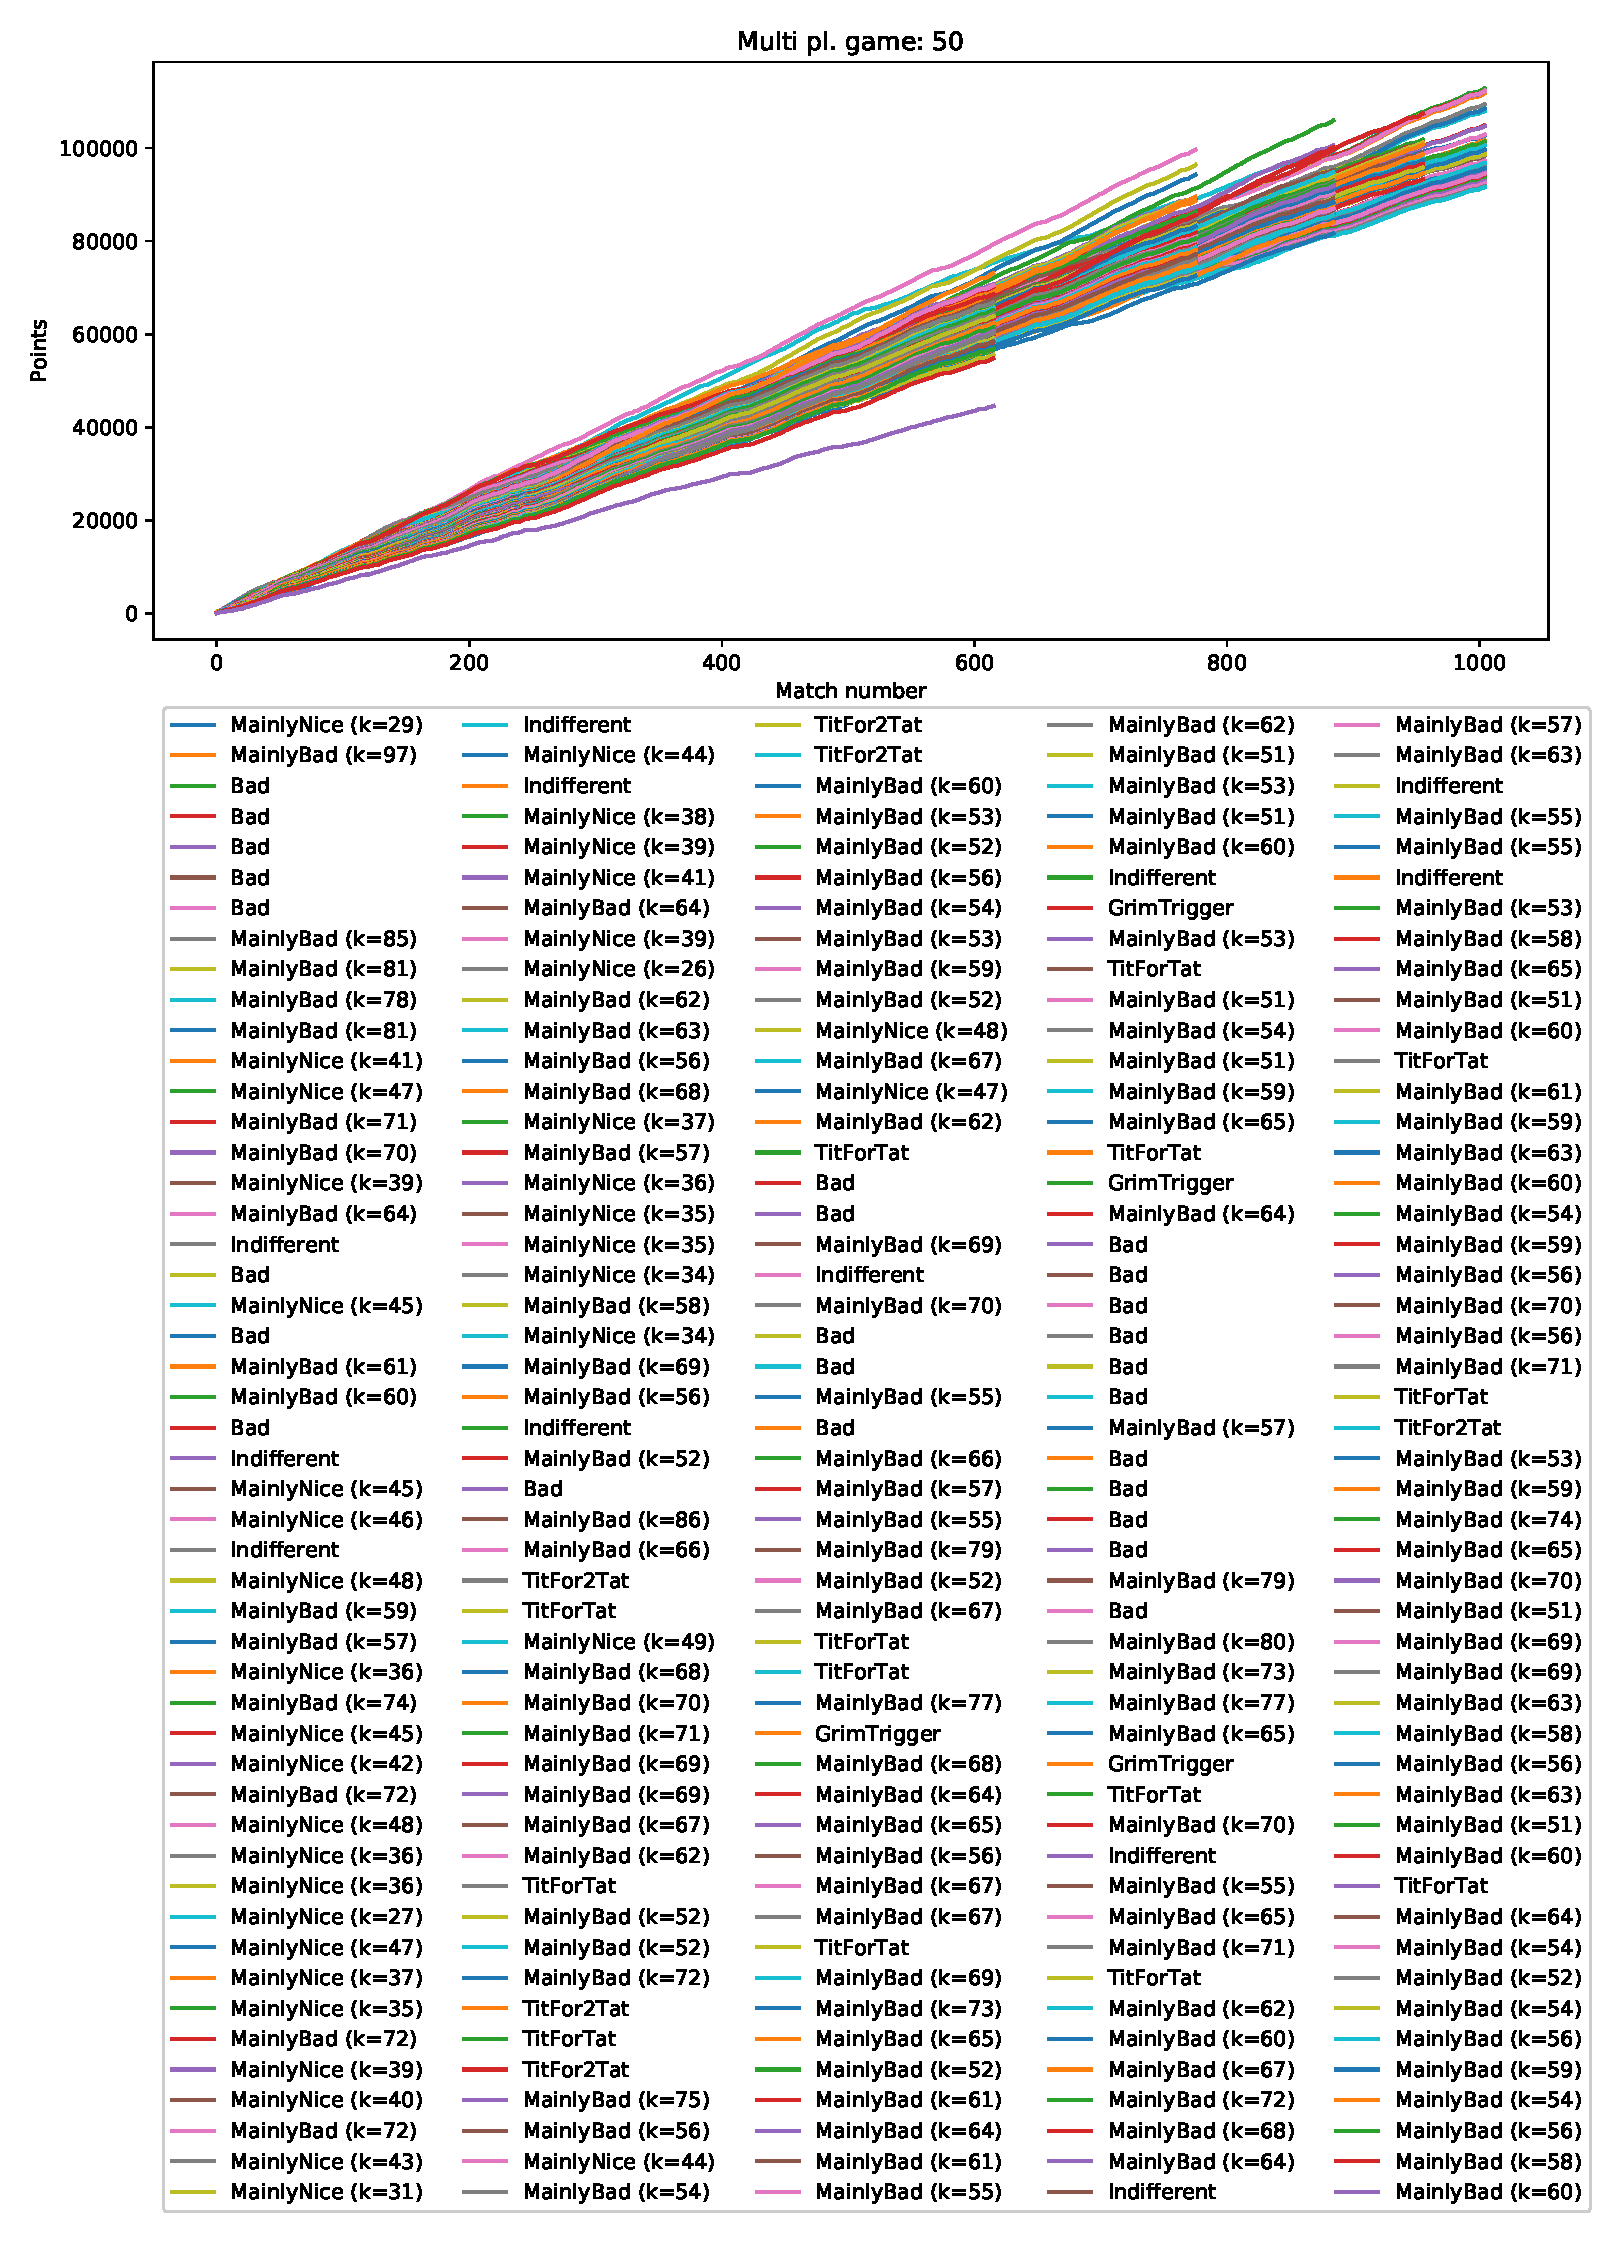
\includegraphics[width=.7\columnwidth]{../img/cipdmp-incr/alt2/cipdmp-scores-increasing-pop-50-r4}
%    \caption{Last iteration scores ($it=4$) (alternative 2)}
%    \label{fig:incrCLI2}
%\end{figure}

\end{document}
